%
% This is an example LaTeX file which uses the SANDreport class file.
% It shows how a SAND report should be formatted, what sections and
% elements it should contain, and how to use the SANDreport class.
% It uses the LaTeX article class, but not the strict option.
% ItINLreport uses .eps logos and files to show how pdflatex can be used
%
% Get the latest version of the class file and more at
%    http://www.cs.sandia.gov/~rolf/SANDreport
%
% This file and the SANDreport.cls file are based on information
% contained in "Guide to Preparing {SAND} Reports", Sand98-0730, edited
% by Tamara K. Locke, and the newer "Guide to Preparing SAND Reports and
% Other Communication Products", SAND2002-2068P.
% Please send corrections and suggestions for improvements to
% Rolf Riesen, Org. 9223, MS 1110, rolf@cs.sandia.gov
%
\documentclass[pdf,12pt]{INLreport}
% pslatex is really old (1994).  It attempts to merge the times and mathptm packages.
% My opinion is that it produces a really bad looking math font.  So why are we using it?
% If you just want to change the text font, you should just \usepackage{times}.
% \usepackage{pslatex}
\usepackage{times}
\usepackage[FIGBOTCAP,normal,bf,tight]{subfigure}
\usepackage{amsmath}
\usepackage{amssymb}
\usepackage{soul}
\usepackage{pifont}
\usepackage{enumerate}
\usepackage{listings}
\usepackage{fullpage}
\usepackage{xcolor}          % Using xcolor for more robust color specification
\usepackage{ifthen}          % For simple checking in newcommand blocks
\usepackage{textcomp}
\usepackage{mathtools}
\usepackage{relsize}
\usepackage{lscape}
\usepackage[toc,page]{appendix}
\usepackage{RAVEN}

\newtheorem{mydef}{Definition}
\newcommand{\norm}[1]{\lVert#1\rVert}
%\usepackage[table,xcdraw]{xcolor}
%\usepackage{authblk}         % For making the author list look prettier
%\renewcommand\Authsep{,~\,}

% Custom colors
\definecolor{deepblue}{rgb}{0,0,0.5}
\definecolor{deepred}{rgb}{0.6,0,0}
\definecolor{deepgreen}{rgb}{0,0.5,0}
\definecolor{forestgreen}{RGB}{34,139,34}
\definecolor{orangered}{RGB}{239,134,64}
\definecolor{darkblue}{rgb}{0.0,0.0,0.6}
\definecolor{gray}{rgb}{0.4,0.4,0.4}

\lstset {
  basicstyle=\ttfamily,
  frame=single
}


\setcounter{secnumdepth}{5}
\lstdefinestyle{XML} {
    language=XML,
    extendedchars=true,
    breaklines=true,
    breakatwhitespace=true,
%    emph={name,dim,interactive,overwrite},
    emphstyle=\color{red},
    basicstyle=\ttfamily,
%    columns=fullflexible,
    commentstyle=\color{gray}\upshape,
    morestring=[b]",
    morecomment=[s]{<?}{?>},
    morecomment=[s][\color{forestgreen}]{<!--}{-->},
    keywordstyle=\color{cyan},
    stringstyle=\ttfamily\color{black},
    tagstyle=\color{darkblue}\bf\ttfamily,
    morekeywords={name,type},
%    morekeywords={name,attribute,source,variables,version,type,release,x,z,y,xlabel,ylabel,how,text,param1,param2,color,label},
}
\lstset{language=python,upquote=true}

\usepackage{titlesec}
\newcommand{\sectionbreak}{\clearpage}
\setcounter{secnumdepth}{4}

%\titleformat{\paragraph}
%{\normalfont\normalsize\bfseries}{\theparagraph}{1em}{}
%\titlespacing*{\paragraph}
%{0pt}{3.25ex plus 1ex minus .2ex}{1.5ex plus .2ex}

%%%%%%%% Begin comands definition to input python code into document
\usepackage[utf8]{inputenc}

% Default fixed font does not support bold face
\DeclareFixedFont{\ttb}{T1}{txtt}{bx}{n}{9} % for bold
\DeclareFixedFont{\ttm}{T1}{txtt}{m}{n}{9}  % for normal

\usepackage{listings}

% Python style for highlighting
\newcommand\pythonstyle{\lstset{
language=Python,
basicstyle=\ttm,
otherkeywords={self, none, return},             % Add keywords here
keywordstyle=\ttb\color{deepblue},
emph={MyClass,__init__},          % Custom highlighting
emphstyle=\ttb\color{deepred},    % Custom highlighting style
stringstyle=\color{deepgreen},
frame=tb,                         % Any extra options here
showstringspaces=false            %
}}


% Python environment
\lstnewenvironment{python}[1][]
{
\pythonstyle
\lstset{#1}
}
{}

% Python for external files
\newcommand\pythonexternal[2][]{{
\pythonstyle
\lstinputlisting[#1]{#2}}}

\lstnewenvironment{xml}
{}
{}

% Python for inline
\newcommand\pythoninline[1]{{\pythonstyle\lstinline!#1!}}

% Named Colors for the comments below (Attempted to match git symbol colors)
\definecolor{RScolor}{HTML}{8EB361}  % Sonat (adjusted for clarity)
\definecolor{DPMcolor}{HTML}{E28B8D} % Dan
\definecolor{JCcolor}{HTML}{82A8D9}  % Josh (adjusted for clarity)
\definecolor{AAcolor}{HTML}{8D7F44}  % Andrea
\definecolor{CRcolor}{HTML}{AC39CE}  % Cristian
\definecolor{RKcolor}{HTML}{3ECC8D}  % Bob (adjusted for clarity)
\definecolor{DMcolor}{HTML}{276605}  % Diego (adjusted for clarity)
\definecolor{PTcolor}{HTML}{990000}  % Paul

\def\DRAFT{} % Uncomment this if you want to see the notes people have been adding
% Comment command for developers (Should only be used under active development)
\ifdefined\DRAFT
  \newcommand{\nameLabeler}[3]{\textcolor{#2}{[[#1: #3]]}}
\else
  \newcommand{\nameLabeler}[3]{}
\fi
\newcommand{\alfoa}[1] {\nameLabeler{Andrea}{AAcolor}{#1}}
\newcommand{\cristr}[1] {\nameLabeler{Cristian}{CRcolor}{#1}}
\newcommand{\mandd}[1] {\nameLabeler{Diego}{DMcolor}{#1}}
\newcommand{\maljdan}[1] {\nameLabeler{Dan}{DPMcolor}{#1}}
\newcommand{\cogljj}[1] {\nameLabeler{Josh}{JCcolor}{#1}}
\newcommand{\bobk}[1] {\nameLabeler{Bob}{RKcolor}{#1}}
\newcommand{\senrs}[1] {\nameLabeler{Sonat}{RScolor}{#1}}
\newcommand{\talbpaul}[1] {\nameLabeler{Paul}{PTcolor}{#1}}
% Commands for making the LaTeX a bit more uniform and cleaner
\newcommand{\TODO}[1]    {\textcolor{red}{\textit{(#1)}}}
\newcommand{\xmlAttrRequired}[1] {\textcolor{red}{\textbf{\texttt{#1}}}}
\newcommand{\xmlAttr}[1] {\textcolor{cyan}{\textbf{\texttt{#1}}}}
\newcommand{\xmlNodeRequired}[1] {\textcolor{deepblue}{\textbf{\texttt{<#1>}}}}
\newcommand{\xmlNode}[1] {\textcolor{darkblue}{\textbf{\texttt{<#1>}}}}
\newcommand{\xmlString}[1] {\textcolor{black}{\textbf{\texttt{'#1'}}}}
\newcommand{\xmlDesc}[1] {\textbf{\textit{#1}}} % Maybe a misnomer, but I am
                                                % using this to detail the data
                                                % type and necessity of an XML
                                                % node or attribute,
                                                % xmlDesc = XML description
\newcommand{\default}[1]{~\\*\textit{Default: #1}}
\newcommand{\nb} {\textcolor{deepgreen}{\textbf{~Note:}}~}


%%%%%%%% End comands definition to input python code into document

%\usepackage[dvips,light,first,bottomafter]{draftcopy}
%\draftcopyName{Sample, contains no OUO}{70}
%\draftcopyName{Draft}{300}

% The bm package provides \bm for bold math fonts.  Apparently
% \boldsymbol, which I used to always use, is now considered
% obsolete.  Also, \boldsymbol doesn't even seem to work with
% the fonts used in this particular document...
\usepackage{bm}


% Define tensors to be in bold math font.
\newcommand{\tensor}[1]{{\bm{#1}}}

% Override the formatting used by \vec.  Instead of a little arrow
% over the letter, this creates a bold character.
\renewcommand{\vec}{\bm}

% Define unit vector notation.  If you don't override the
% behavior of \vec, you probably want to use the second one.
\newcommand{\unit}[1]{\hat{\bm{#1}}}
% \newcommand{\unit}[1]{\hat{#1}}

% Use this to refer to a single component of a unit vector.
\newcommand{\scalarunit}[1]{\hat{#1}}

% \toprule, \midrule, \bottomrule for tables
\usepackage{booktabs}

% \llbracket, \rrbracket
\usepackage{stmaryrd}

\usepackage{hyperref}
\hypersetup{
    colorlinks,
    citecolor=black,
    filecolor=black,
    linkcolor=black,
    urlcolor=black
}

% Compress lists of citations like [33,34,35,36,37] to [33-37]
\usepackage{cite}

% If you want to relax some of the SAND98-0730 requirements, use the "relax"
% option. It adds spaces and boldface in the table of contents, and does not
% force the page layout sizes.
% e.g. \documentclass[relax,12pt]{SANDreport}
%
% You can also use the "strict" option, which applies even more of the
% SAND98-0730 guidelines. It gets rid of section numbers which are often
% useful; e.g. \documentclass[strict]{SANDreport}

% The INLreport class uses \flushbottom formatting by default (since
% it's intended to be two-sided document).  \flushbottom causes
% additional space to be inserted both before and after paragraphs so
% that no matter how much text is actually available, it fills up the
% page from top to bottom.  My feeling is that \raggedbottom looks much
% better, primarily because most people will view the report
% electronically and not in a two-sided printed format where some argue
% \raggedbottom looks worse.  If we really want to have the original
% behavior, we can comment out this line...
\raggedbottom
\setcounter{secnumdepth}{5} % show 5 levels of subsection
\setcounter{tocdepth}{5} % include 5 levels of subsection in table of contents

% ---------------------------------------------------------------------------- %
%
% Set the title, author, and date
%
\title{RAVEN User Guide}
%\author{%
%\begin{tabular}{c} Author 1 \\ University1 \\ Mail1 \\ \\
%Author 3 \\ University3 \\ Mail3 \end{tabular} \and
%\begin{tabular}{c} Author 2 \\ University2 \\ Mail2 \\ \\
%Author 4 \\ University4 \\ Mail4\\
%\end{tabular} }


\author{
\\Andrea Alfonsi
\\Cristian Rabiti
\\Diego Mandelli
\\Joshua Cogliati
\\Congjian Wang
\\Paul W. Talbot
\\Daniel P. Maljovec
\\Curtis Smith
}
%Just people who actually ``developed'' a significant capability in the code should be placed here. Andrea
%\author{\textbf{\textit{Main Developers:}}  \\Andrea Alfonsi}
%\affil{Idaho National Laboratory, Idaho Falls, ID 83402}
%\\\{cristian.rabiti, andrea.alfonsi, joshua.cogliati, diego.mandelli, robert.kinoshita, ramazan.sen\}@inl.gov}

% There is a "Printed" date on the title page of a SAND report, so
% the generic \date should [WorkingDir:]generally be empty.
\date{}


% ---------------------------------------------------------------------------- %
% Set some things we need for SAND reports. These are mandatory
%
\SANDnum{INL/EXT-16-38178}
\SANDprintDate{March 2017}
\SANDauthor{Andrea Alfonsi, Cristian Rabiti, Diego Mandelli, Joshua Cogliati, Congjian Wang, Paul W. Talbot, Daniel P. Maljovec, Curtis Smith}
\SANDreleaseType{Revision 2 draft}


% ---------------------------------------------------------------------------- %
% Include the markings required for your SAND report. The default is "Unlimited
% Release". You may have to edit the file included here, or create your own
% (see the examples provided).
%
% \include{MarkOUO} % Not needed for unlimted release reports

\def\component#1{\texttt{#1}}

% ---------------------------------------------------------------------------- %
\newcommand{\systemtau}{\tensor{\tau}_{\!\text{SUPG}}}

% Added by Sonat
\usepackage{placeins}
\usepackage{array}

\newcolumntype{L}[1]{>{\raggedright\let\newline\\\arraybackslash\hspace{0pt}}m{#1}}
\newcolumntype{C}[1]{>{\centering\let\newline\\\arraybackslash\hspace{0pt}}m{#1}}
\newcolumntype{R}[1]{>{\raggedleft\let\newline\\\arraybackslash\hspace{0pt}}m{#1}}

% end added by Sonat
% ---------------------------------------------------------------------------- %
%
% Start the document
%

\begin{document}

    \maketitle

    % ------------------------------------------------------------------------ %
    % An Abstract is required for SAND reports
    %
%    \begin{abstract}
%    \input abstract
%    \end{abstract}


    % ------------------------------------------------------------------------ %
    % An Acknowledgement section is optional but important, if someone made
    % contributions or helped beyond the normal part of a work assignment.
    % Use \section* since we don't want it in the table of context
    %
%    \clearpage
%    \section*{Acknowledgment}



%	The format of this report is based on information found
%	in~\cite{Sand98-0730}.


    % ------------------------------------------------------------------------ %
    % The table of contents and list of figures and tables
    % Comment out \listoffigures and \listoftables if there are no
    % figures or tables. Make sure this starts on an odd numbered page
    %
    \cleardoublepage		% TOC needs to start on an odd page
    \tableofcontents
    %\listoffigures
    %\listoftables


    % ---------------------------------------------------------------------- %
    % An optional preface or Foreword
%    \clearpage
%    \section*{Preface}
%    \addcontentsline{toc}{section}{Preface}
%	Although muggles usually have only limited experience with
%	magic, and many even dispute its existence, it is worthwhile
%	to be open minded and explore the possibilities.


    % ---------------------------------------------------------------------- %
    % An optional executive summary
    %\clearpage
    %\section*{Summary}
    %\addcontentsline{toc}{section}{Summary}
    %\input{Summary.tex}
%	Once a certain level of mistrust and skepticism has
%	been overcome, magic finds many uses in todays science



%	and engineering. In this report we explain some of the
%	fundamental spells and instruments of magic and wizardry. We
%	then conclude with a few examples on how they can be used
%	in daily activities at national Laboratories.


    % ---------------------------------------------------------------------- %
    % An optional glossary. We don't want it to be numbered
%    \clearpage
%    \section*{Nomenclature}
%    \addcontentsline{toc}{section}{Nomenclature}
%    \begin{description}
%          \item[alohomoral]
%           spell to open locked doors and containers
%          \item[leviosa]
%           spell to levitate objects
%    \item[remembrall]
%           device to alert you that you have forgotten something
%    \item[wand]
%           device to execute spells
%    \end{description}


    % ---------------------------------------------------------------------- %
    % This is where the body of the report begins; usually with an Introduction
    %
    \SANDmain		% Start the main part of the report

\section{Introduction}
% High-level RAVEN description
RAVEN~\cite{alfonsiMC} ~\cite{alfonsiPSA}~\cite{RAVENFY13}~\cite{ESREL2014} is a software framework that allows the user to perform parametric and stochastic
analysis based on the response of complex system codes.
The initial development was designed to provide dynamic probabilistic risk analysis
capabilities (DPRA) to the thermal-hydraulic code RELAP-7~\cite{relap7FY12}, currently under development
at Idaho National Laboratory (INL).
Now, RAVEN is not only a framework to perform DPRA but it is a
multi-purpose stochastic and uncertainty quantification platform, capable of communicating with any system code.

The provided Application Programming
Interfaces (APIs) allow RAVEN to interact with any code as long as all the parameters
that need to be perturbed are accessible by input files or via python
interfaces.
RAVEN is capable of investigating system response and explore input space using various
sampling schemes such as Monte Carlo, grid, or Latin Hypercube.
However, RAVEN strength lies in its system feature discovery capabilities such as: constructing
limit surfaces, separating regions of the input space leading to system failure,
and using dynamic supervised learning techniques.

The development of RAVEN started in 2012 when, within the Nuclear Energy
Advanced Modeling and Simulation (NEAMS) program~\cite{neams}, the need of a modern
risk evaluation framework arose.
RAVEN's principal assignment is to provide the necessary software and algorithms
in order to employ the concepts developed by the Risk Informed Safety Margin
Characterization (RISMC) Pathway.
RISMC is one of the pathways defined within the Light Water Reactor
Sustainability (LWRS) program~\cite{lwrs}.

The goal of the RISMC approach is  the identification not only of the frequency of an
event which can potentially lead to system failure, but also the proximity (or lack
thereof) to key safety-related events: the safety margin.
Hence, the approach is interested in identifying and increasing the safety
margins related to those events.
A safety margin is a numerical value quantifying the probability that a safety
metric (e.g. peak pressure in a pipe) is exceeded under certain conditions.
% Conclusion
Most of the capabilities, implemented having Reactor Excursion and Leak Analysis Program v.7
(RELAP-7) as a principal focus, are
easily deployable to other system codes.
%
For this reason, several side activates have been employed (e.g.  RELAP5-3D~\cite{RELAP5userManual}, any Multiphysics Object Oriented
Simulation Environment-based App, etc.)
or are currently ongoing for coupling RAVEN with several different software.
%
The aim of this document is to provide a set of detailed examples that can help the user to become familiar with the RAVEN code.

\section{RAVEN Tutorial}
\label{sec:ravenTutorial}

% A simple example
\subsection{Example Model: Analytic Bateman}\label{sec:analyticalbateman}
This section is intended for the new users to familiarize them with how to perform their studies through RAVEN.
A simple example, conventionally called \textbf{AnalyticBateman}, has been developed. It solves a system of
ordinary differential equations (ODEs), of the form:

\begin{equation}
\begin{dcases}
\frac{\mathrm{d} \mathbf{X}}{\mathrm{d} t} = \mathbf{S}-\mathbf{L} \\
 \mathbf{X}(t=0)= \mathbf{X_{0}}
\end{dcases}
\end{equation}
   where:
  \begin{itemize}
     \item $\mathbf{X_{0}}$, initial conditions
     \item $\mathbf{S}$, source terms
     \item $\mathbf{L}$, loss terms
   \end{itemize}

For example, this  code is able to solve a system of two ODEs as follows:
\begin{equation}
  \begin{dcases}
    \frac{\mathrm{d} x_{1}}{\mathrm{d} t} = \phi (t)\times \sigma_{x_{1}}-\lambda_{x_{1}}\times x_{1}(t) \\
    \frac{\mathrm{d} x_{2}}{\mathrm{d} t} = \phi (t)\times \sigma_{x_{2}}-\lambda_{x_{2}} \times x_{2}(t) + x_{1}(t)\times\lambda_{x_{1}} \\
    x_{1}(t=0)= x_{1}^{0} \\
    x_{2}(t=0)= 0.0
  \end{dcases}
\end{equation}

The input of the \textbf{AnalyticBateman} code is in XML format.
For example, the following is the reference input for a system of 4 Ordinary Differential Equations (ODEs)
that is going to be used for as an example in this guide. All the files required for this system are  located at
``\textit{raven/tests/framework/user\textunderscore guide/physicalCode}''. 

\xmlExample{framework/user_guide/physicalCode/analyticalbateman/Input.xml}{AnalyticalBateman}
The code outputs the time evolution of the 4 variables ($A,B,C,D$) in a CSV file, producing the following output:
\begin{table}[ht]
\centering
\caption{Reference case sample results.}
\label{referenceResults}
\begin{tabular}{lllll}
\textbf{time} & \textbf{A}     & \textbf{C}     & \textbf{B}    & \textbf{D}     \\
0                  & 1.0                       & 1.0                       & 1.0                     & 1.0           \\
2880000.0   & 0.983434738239 & 0.977851848235 & 1.01011506729 & 1.01013172275 \\
5760000.0   & 0.967143884376 & 0.956202457404 & 1.01936231677 & 1.02036100400   \\
8640000.0   & 0.951122892771 & 0.935040450532 & 1.02777406275 & 1.03067925987 \\
10368000.0 & 0.941637968936 & 0.922572556179 & 1.03243314106 & 1.03690947068 \\
12096000.0 & 0.932247632016 & 0.910273757371 & 1.03680933440 & 1.04316700086 \\
13824000.0 & 0.922950938758 & 0.898141730426 & 1.04090912054 & 1.04945015916 \\
15552000.0 & 0.913746955315 & 0.886174183908 & 1.04473885709 & 1.05575729317 \\
17280000.0 & 0.904634757153 & 0.874368858183 & 1.04830478357 & 1.06208678854 \\
20736000.0 & 0.886682064542 & 0.851235986899 & 1.05466958557 & 1.07480659230  \\
24192000.0 & 0.869085647400 & 0.828725658721 & 1.06005115510 & 1.08759739100   \\
27648000.0 & 0.851838435355 & 0.806820896763 & 1.06449535534 & 1.10044757060  \\
31104000.0 & 0.834933498348 & 0.785505191756 & 1.06804634347 & 1.11334606143 \\
34560000.0 & 0.818364043850 & 0.764762489077 & 1.07074662835 & 1.12628231792
\end{tabular}
\end{table}

% Run RAVEN with the simple example, and build RAVEN input with explanation
% Include SingleRun and IOStep
\section{Run a Single Instance of a Code and Load the Outputs}
The simplest exercise that can be performed is to run the driven code (\textbf{AnalyticBateman}  in our example), loading the results of a single run into RAVEN, printing and plotting some variables.
\\ As detailed in the RAVEN user manual (~\cite{RAVENuserManual}-Chapters ``DataObjects''  and ``Databases'') and in Chapter~\ref{sub:EntitiesAndFlow} RAVEN uses two classes of objects to store the data coming from a driven code (outputs):
\begin{itemize}
  \item \textbf{DataObjects}: The DataObjects represent the preferred way to transfer the information coming from a
   Model (the driven code, in this case) to all the other RAVEN systems (e.g. Out-Stream system, Reduced Order Modeling
   component, etc.).
  \item \textbf{Databases}.
\end{itemize}

As inferable from the user manual (~\cite{RAVENuserManual}-Chapter ``OutStream''), the DataObjects can be exported into a CSV file and plotted (2-D and 3-D plots) linking them into the OutStream system.
\\ The following subsections report examples on how to use these systems running a single instance of the driven code.
\subsection{Single Run using the OutStream system for printing and create basic plots}
\label{sub:SingleRunBasicPlots}
 In this Section, the user can learn how to use RAVEN to run a single instance of a driven code, plotting and printing the
 results.
 \\ The goal of this Section is to learn how to:
 \begin{enumerate}
   \item Set up a simple RAVEN input for running a driven code;
   \item Load the output of the code into the RAVEN DataObjects system;
   \item Print out what contained in the DataObjects;
   \item Generate basic plots of the code results.
\end{enumerate}
In order to accomplish these tasks, the following RAVEN \textbf{Entities} (XML blocks in the input files) are needed:
 \begin{enumerate}
   \item \textbf{\textit{RunInfo}}:
     \xmlExample{framework/user_guide/SingleRuns/singleRunPlotAndPrint-VI.I.xml}{RunInfo}
   As given in Section~\ref{sub:EntitiesAndFlow}, the \textit{RunInfo} \textbf{Entity} is intended to set up the analysis
   that the user wants to perform. In this specific case, two steps (\xmlNode{Sequence}) are going to be sequentially run
   using a single processor (\xmlNode{batchSize}).

   \item \textbf{\textit{Files}}:
     \xmlExample{framework/user_guide/SingleRuns/singleRunPlotAndPrint-VI.I.xml}{Files}
   Since the driven code uses a single input file, in this Section the original input is placed. As described in the user manual~\cite{}
   the attribute  \xmlAttr{name} represents the alias that is going to be used in all the other input blocks in order to
   refer to this file.
   \item \textbf{\textit{Models}}:
     \xmlExample{framework/user_guide/SingleRuns/singleRunPlotAndPrint-VI.I.xml}{Models}
  Since the driven code already dumps its outputs in CSV format, there is no need to create
  an ad-hoc code interface and the GenericCode interface can be directly used. In additiom, since the \textbf{AnalyticBateman} code
  is written in \texttt{Python}, it is necessary to specify that the code needs to be run pre-pending the expression ``\texttt{Python}''.
   \item \textbf{\textit{DataObjects}}:
     \xmlExample{framework/user_guide/SingleRuns/singleRunPlotAndPrint-VI.I.xml}{DataObjects}
  Int this block, two \textit{DataObjects} are defined: 1) PointSet named ``pointValues'', 2) HistorySet named ``history''.
  Note that a special keyword is inputted in the \xmlNode{Input} node. This keyword is used when a \textit{DataObjects}  \textbf{Entity} needs to be constructed without any linking with respect to the input space. Indeed, in
  this case, the model input space is not perturbed though a sampling strategies; the code is executed through the original
   input file   (``referenceInput.xml''). In the \xmlNode{Output} node all the requested variables are inputted.
   \item \textbf{\textit{OutStreams}}:
     \xmlExample{framework/user_guide/SingleRuns/singleRunPlotAndPrint-VI.I.xml}{OutStreams}
  In this block, both the Out-Stream types are constructed:
  \begin{itemize}
    \item \textit{Print}:
     \begin{itemize}
       \item named ``pointValues'' connected with the \textit{DataObjects} \textbf{Entity} ``pointValues''
                (\xmlNode{source})
       \item named ``history'' connected with the \textit{DataObjects} \textbf{Entity} ``history'' (\xmlNode{source})
     \end{itemize}
      When this objects get used, all the information contained in the linked  \textit{DataObjects} are going
    to be dumped in CSV files (\xmlNode{type}).
    \item \textit{Plot}: a single \xmlNode{Plot} \textbf{Entity} is defined, containing the line plots of the 4 output variables
    ($A,B,C,D$) in the same figure. This object is going to generate a PNG file and an interactive Plot on
    the screen.
  \end{itemize}
   \item \textbf{\textit{Steps}}:
     \xmlExample{framework/user_guide/SingleRuns/singleRunPlotAndPrint-VI.I.xml}{Steps}
 %%%%%%%%%%%%%%%%%%%%%%%%%%%%%%%%%%%%%%%%%%%%%%%%%%%%%%%%%%
 %figure history
 \begin{figure}[h!]
  \centering
  \includegraphics[scale=0.7]{../../tests/framework/user_guide/SingleRuns/gold/sectionVI.I/1-historyPlot_line-line-line-line.png}
  \caption{Plot of the history for variables $A,B,C,D$.}
  \label{fig:historyPlotLine}
 \end{figure}
 %%%%%%%%%%%%%%%%%%%%%%%%%%%%%%%%%%%%%%%%%%%%%%%%%%%%%%%%%%
   Finally, all the previously defined \textbf{Entities} can be combined in the \xmlNode{Steps} block. Thus,
   two \xmlNode{Steps} have been inputted:
   \begin{itemize}
     \item \xmlNode{SingleRun} named ``Single'', used to run the single instance of the driven code and collect
     the outputs in the two \textit{DataObjects}. In addition, it can be seen that an additional object has been
     placed among the \xmlNode{Output}(s). Indeed, an  \textit{OutStreams} can be an \xmlNode{Output} in
     any Step type (as long as the linked \textit{DataObjects} plays a whatever role in the Step)
     \item  \xmlNode{IOStep} named ``writeHistory'', used to 1) dump the ``history'' \textit{DataObjects}
     \textbf{Entity} in a CSV file and 2) plot the data in the PNG file and on the screen.
   \end{itemize}
\end{enumerate}
For examples of the numerical data produced by the OutStreams \textit{Print}, see \texttt{history\_0.csv} and
\texttt{pointValues.csv} in the directory
 \texttt{raven/tests/framework/user\_guide/SingleRuns/gold/sectionVI.I/}
 As previously mentioned, Figure~\ref{fig:historyPlotLine} reports the four plots (four variables) drawn in the same picture.

%\FloatBarrier
\subsection{Single Run using the OutStream System to Sub-plot and Selectively print.}
This Section shows how to use RAVEN to create sub-plots (multiple plots in the same figure) and
how to select only some variable from the \textit{DataObjects} in the \textit{Print} OutStream.
 \\ The goals of this Section are about learning how to:
 \begin{enumerate}
   \item Print out what contained in the DataObjects, selecting only few variables
   \item Generate sub-plots (multiple plots in the same figure) of the code results
\end{enumerate}

To accomplish these tasks, the \textit{OutStreams} \textbf{Entity} in the input defined in the previous Section (~\ref{sub:SingleRunBasicPlots}) needs to be modified as follows:
\xmlExample{framework/user_guide/SingleRuns/singleRunSubPlotsAndSelectivePrint-VI.II.xml}{OutStreams}
\begin{enumerate}
   \item \textbf{\textit{Print}}:
   With respect to the \textit{Print} nodes defined in the previous Section (~\ref{sub:SingleRunBasicPlots}), it can
   be noticed that an additional node has been added: \xmlNode{what}. The \textit{Print} \textbf{Entity}
   ``pointValues'' is going to extract and dump only the variables that are part of the Output space
   ($A,B,C,D$ and not $InputPlaceHolder$).  The \textit{Print} \textbf{Entity} ``history'' is instead going to print
   the Output space variables $A$ and $D$.

   \item \textbf{\textit{Plot}}:
 Note that the  \textit{Plot} \textbf{Entity} does not differ much with respect to the one in
 Section~\ref{sub:SingleRunBasicPlots}: 1) the additional sub-node \xmlNode{gridSpace}  has been added.
 This node is needed to define how the figure needs to be partitioned (discretization of the grid). In this case
 a 2 by 2 grid is requested. 2) in each \xmlNode{plot} the node \xmlNode{gridLocation} is placed in
 order to specify in which position the relative plot needs to be placed. For example, in the following grid
 location, the relative plot is going to be placed at the bottom-right corner.
  \begin{lstlisting}[style=XML,morekeywords={arg,extension,pauseAtEnd,overwrite}]
   <gridLocation>
      <x>1</x>
      <y>1</y>
   </gridLocation>
   \end{lstlisting}
 \end{enumerate}
The CSV tables generated by the \textit{Print} \textbf{Entities} are not reported, since the only differences with respect to Tables ~\ref{historyVI.I} and ~\ref{pointValuesVI.I} are related to the number of columns (variables)
dumped out.
\\Figure~\ref{fig:historySubPlotLine} reports the four plots (four variables) drawn in the same picture.
 %figure history sublots
 \begin{figure}[h!]
  \centering
  \includegraphics[scale=0.7]{../../tests/framework/user_guide/SingleRuns/gold/sectionVI.II/1-historyPlot_line-line-line-line.png}
  \caption{Subplot of the history for variables $A,B,C,D$.}
  \label{fig:historySubPlotLine}
 \end{figure}


% MultiRun
\subsection{Build RAVEN Input: \xmlNode{MultiRun}}
\label{sub:tutorialMultiRun}
The \textbf{MultiRun} step allows the user to assemble the calculation flow of an analysis that requires multiple
``runs'' of the same model. This step is used, for example, when the input (space) of the model needs to be
perturbed by a particular sampling strategy. In the \xmlNode{MultiRun} input block, the user needs to specify the
objects that need to be used for the different allowable roles. This step accepts the following roles:

\begin{itemize}
  \item \textit{Input}
  \item \textit{Model}
  \item \textit{Output}
  \item \textit{Sampler}
  \item \textit{Optimizer}
  \item \textit{SolutionExport}
\end{itemize}

\textbf{MultiRun} is intended to handle calculations that involve multiple runs of a driven code (sampling strategies).
Firstly, the RAVEN input file associates the variables to a set of PDFs and to a sampling strategy. The ``multi-run''
step is used to perform several runs in a block of a model (e.g. in a MC sampling).

\begin{figure}[ht]
  \centering
  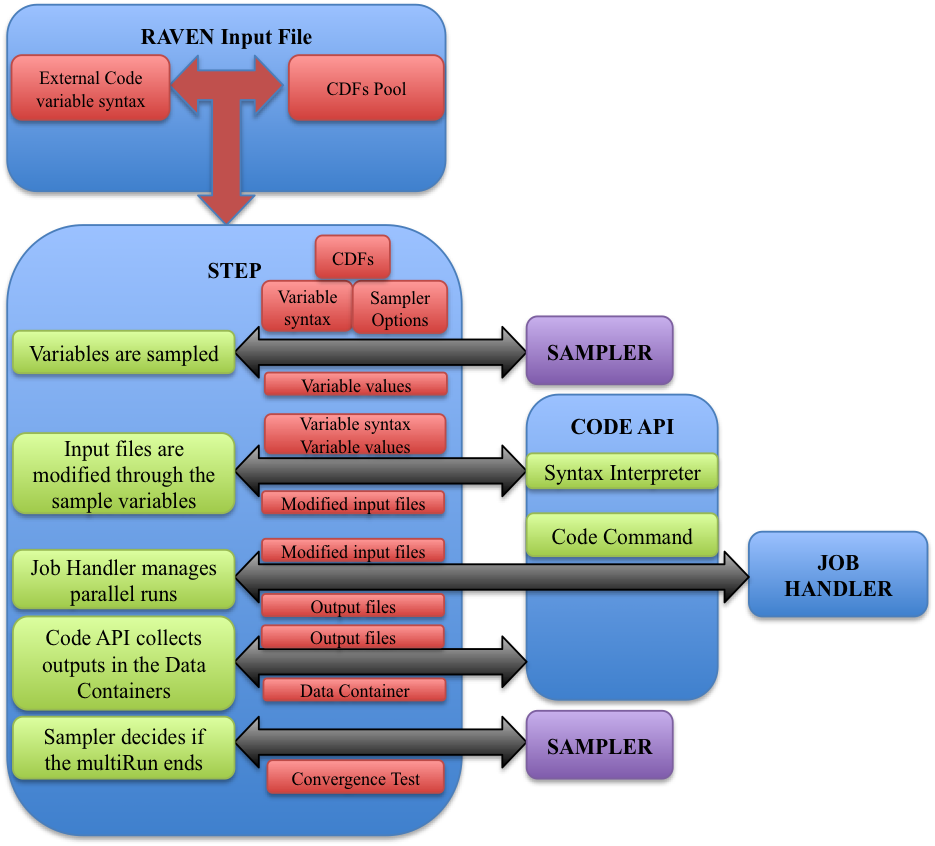
\includegraphics[width=0.8\textwidth]  {pics/MultiRunCalculationFlow.png}
  \caption{Calculation flow for a multi-run sampling}
  \label{fig:multiRun}
\end{figure}

As shown in Figure~\ref{fig:multiRun}, at the beginning of each sub sequential run, the sampler provides the new values of the variables to be perturbed.
The code API places those values in the input file. At this point, the code API generates the run command and asks
to be queued by the job handler. The job handler manages the parallel execution of as many runs as possible within
a user prescribed range and communicates with the step controller when a new set of output files are ready to be
processed. The code API receives the new input files and collects the data in the RAVEN internal format. The sampler
is queried to assess if the sequence of runs is ended, if not, the step controller asks for a new set of values
from the sampler and the sequence is restarted.
The job handler is currently capable to run different run instances of the code in parallel and can also handle
codes that are multi-threaded or using any form of parallel implementation.
RAVEN also has the capability to plot the simulation outcomes while the set of sampling is performed and to store
the data for later recovery.

In this section, we will show the user how to set up the \textit{Sampler}, and employ \textbf{MultiRun} to execute
all perturbed models. The use of \textit{Optimizer} and \textit{SolutionExport} will be introduced in another section.
The \textbf{Samplers}  entity is the container of all the algorithms designed to perform the perturbation of the
input space. The Samplers can be categorized into three main classes:

\begin{itemize}
  \item  \textit{Forward}. Sampling strategies that do not leverage the information coming from already evaluated
    realizations in the input space. For example, Monte-Carlo, Stratified (LHS), Grid, Response Surface, Factorial Design,
    Sparse Grid, etc.
  \item  \textit{Adaptive}. Sampling strategies that take advantages of the information coming from already evaluated
    realizations of the input space, adapting the sampling strategies to key figures of merits. For example, Limit Surface
    search, Adaptive sparse grid, etc.
  \item \textit{Dynamic Event Tree}. Sampling strategies that perform the exploration of the input space based on the
    dynamic evolution of the system, employing branching techniques. For example, Dynamic Event Tree, Hybrid
    Dynamic Event Tree, etc.
\end{itemize}

The sampler is probably the most important entity in the RAVEN framework. It provides many different sampling
strategies that can be used in almost all RAVEN related applications. In this section, we will only illustrate
the simplest forward sampler, i.e. \textit{Monte-Carlo}, to familarize the user with the use of sampler. Monte-Carlo method
is one of the most-used methodologies in several mathematic disciplines. The theory of this method can be found in
the RAVEN theory manual. In addition, we will continue to use the \textbf{AnalyticBateman} to illustrate the setup
of \textbf{MultiRun} and \textbf{Samplers}. In order to accomplish these tasks, the following precedures or RAVEN
entities are needed:

\begin{enumerate}
  \item Set up the running environment: \xmlNode{RunInfo}
  \item Provide the required files: \xmlNode{Files}
  \item Link between RAVEN and dirven code: \xmlNode{Models}
  \item Define probability distribution functions for inputs: \xmlNode{Distributions}
  \item Set up a simple Monte-Carlo sampling for perturbing the input space: \xmlNode{Samplers}
  \item Store the input and output data: \xmlNode{DataObjects}
  \item Print and plot input and output data: \xmlNode{OutStreams}
  \item Control multiple executions: \xmlNode{Steps}
\end{enumerate}

In section~\ref{sub:singleRun}, we have already discussed the use of \xmlNode{RunInfo}, \xmlNode{Files}, \xmlNode{Models},
\xmlNode{DataObjects}, \xmlNode{OutStreams}. For practice, the user can try to build these RAVEN entities by themselves,
and refer to the complete input file located at
\textit{raven/tests/framework/user\_guide/ ravenTutorial/MonteCarlo.xml}.
In this section, we'd like to show the users how to set up \xmlNode{Distributions}, \xmlNode{Samplers} and \textbf{MultiRun}
of \xmlNode{Steps}. RAVEN employs \xmlNode{Distributions} to define many different probability distribution
functions (PDFs) that can be used to characterize the input parameters. One can consider the \xmlNode{Distributions}
entity to be a container of all the stochastic representation of random variables. Currently, RAVEN supports:
\begin{itemize}
  \item \textit{1-Dimensional} continuous and discrete distributions, such as Normal, Weibull, Binomial, etc.
  \item \textit{N-Dimensional} distributions, such as Multivariate Normal, user-inputted N-Dimensional distributions.
\end{itemize}
For the \textbf{AnalyticBateman} example, two 1-D uniform distributions are defined:
\begin{itemize}
  \item $sigma \sim \mathbb{U}(1,10)$, used to model the uncertainties associated with the \textit{sigma} Model variables;
  \item $decayConstant \sim \mathbb{U}(0.5e-8,1e-8)$,  used to model the uncertainties associated with the Model variable
    \textit{decay constants}.  Note that the same distribution can be re-used for multiple input variables, while
    still keeping those variables independent.
\end{itemize}
The following is the definition of \xmlNode{Distributions} block that is used for the \textbf{AnalyticBateman} problem:
\xmlExample{framework/user_guide/ravenTutorial/MonteCarlo.xml}{Distributions}
For uniform distributions, only \xmlNode{lowerBound} and \xmlNode{upperBound} are required. For other distributions,
please refer to the RAVEN user manual.

As we already mentioned, we will employ Monte-Carlo sampling strategy to demonstrate \textbf{MultiRun}.
To employ the Monte-Carlo sampling strategy, a \xmlNode{MonteCarlo} node needs to be defined.
The user also needs to specify the variables that need to be sampled using \xmlNode{variable}. In addition,
the setting for this sampler need to be specified in the \xmlNode{samplerInit} block. The only required sub-node
\xmlNode{limit} is used to specify the number of Monte Carlo samples. The user can also use other optional sub-node
to characterize their samplers. For this example, the \xmlNode{Samplers} block is:
\xmlExample{framework/user_guide/ravenTutorial/MonteCarlo.xml}{Samplers}
In this case, the Monte-Carlo method is employed on $two$ model variables, each of which are listed by name and
are associated with a distribution. Note that the \textit{decay-\*} and \textit{sigma-\*} variables are
associated with the distributions $decayConstant$ and $sigma$, respectively. These variables and their values are
passed to the model via the generic code interface. This requires the users to make some changes in their input files
in order to accept these variables. For example, the input file of \textbf{AnalyticBateman} becomes:
\xmlExample{framework/user_guide/ravenTutorial/commonFiles/referenceInput_generic_CI.xml}{nuclides}
As shown in this example, the values of nodes \xmlNode{sigma} and \xmlNode{decayConstant} are replaced with variables
\xmlString{\$RAVEN-decay-A|10\$} and \xmlString{\$RAVEN-sigma-A|10\$}, respectively. \nb we use prefix \xmlString{RAVEN-}
$+$ \xmlString{variable names defined inside RAVEN input files} within \xmlString{\$ \$} to define the
RAVEN-editable input parameters. In other words, the RAVEN-editable input parameters is used to transfer the sampled values
of RAVEN variables to input parameters of given code. This is the only way to connect the input parameters of code
with variables of RAVEN if \textit{Generic code interface} is employed. In addition, we use the wild-cards \texttt{|}
to define the format of the value of the RAVEN-editable input parameters. In this case, the value that is going to
be replaced by the generic code interface will be left-justified with a string length of 10 (e.g. ``\texttt{|}10''). Other
formatting options can be found in the RAVEN user manual.

As we already mentioned, the \textit{Generic code interface} requires that the codes need to return a CSV file with
the input parameters and output parameters. The filename of the CSV file should includes:
\begin{itemize}
  \item prefix: ``out$\mathtt{\sim}$''
  \item filename: the base of input filename without extension
  \item extension: ``.csv''
\end{itemize}
For this case, the input filename is ``referenceInput\_generic\_CI.xml'', thus the output CSV filename should be
``out$\mathtt{\sim}$referenceInput\_generic\_CI.csv''.

Once all the other entities are defined in the RAVEN input file, they must be combined in the \xmlNode{Steps} block,
which dictates the workflow of RAVEN.  For this case, two \xmlNode{Steps} are defined:
\begin{itemize}
  \item \xmlNode{MultiRun} ``sample'', used to run the multiple instances of the driven code and  collect the outputs
    in the two \textit{DataObjects}. As it can be seen, the \xmlNode{Sampler} is specified to communicate to the
    \textit{Step} that the driven code needs to be perturbed through the Monte-Carlo sampling.
  \item  \xmlNode{IOStep} named ``writeHistories'', used to 1) dump the ``histories'' and ``samples'' \textit{DataObjects}
    \textbf{Entity} to a CSV file and 2) plot the data in the EPS file.
\end{itemize}

Figures~\ref{fig:historiesMCPlotLine_A} and ~\ref{fig:samplesMCPlotLine_A} show the report generated by RAVEN of the
evolution of the variable $A$ and its final values, respectively.
\xmlExample{framework/user_guide/ravenTutorial/MonteCarlo.xml}{Steps}

%%%%%%%%%%%%%%%%%%%%%%%%%%%%%%%%%%%%%%%%%%%%%%%%%%%%%%%%%%
%figure histories
\begin{figure}[h!]
  \centering
  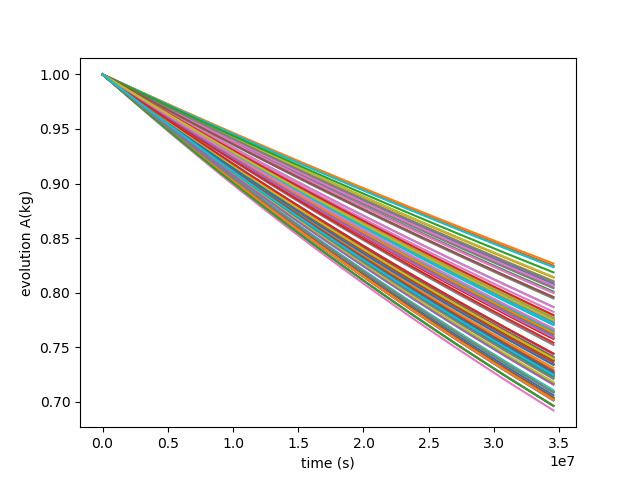
\includegraphics[scale=0.7]{../../tests/framework/user_guide/ravenTutorial/gold/MonteCarlo/1-history_A_line.png}
  \caption{Plot of the histories generated by the Monte Carlo sampling for variable $A$.}
  \label{fig:historiesMCPlotLine_A}
\end{figure}
%%%%%%%%%%%%%%%%%%%%%%%%%%%%%%%%%%%%%%%%%%%%%%%%%%%%%%%%%%
 
%%%%%%%%%%%%%%%%%%%%%%%%%%%%%%%%%%%%%%%%%%%%%%%%%%%%%%%%%%
%figure samples
\begin{figure}[h!]
  \centering
  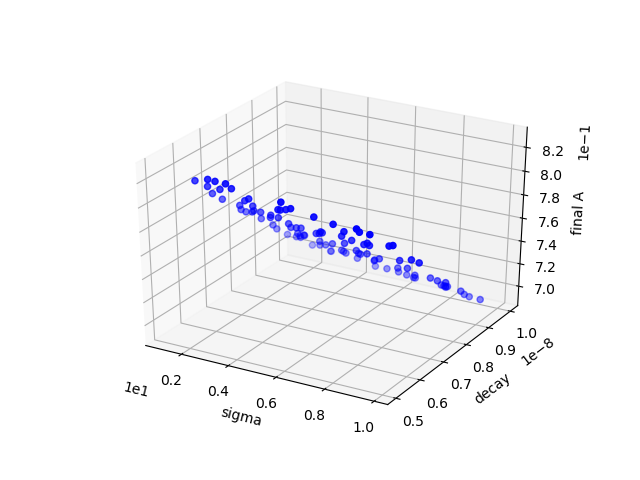
\includegraphics[scale=0.7]{../../tests/framework/user_guide/ravenTutorial/gold/MonteCarlo/1-samplesPlot_A_scatter.png}
  \caption{Plot of the samples generated by the MC sampling for variable $A$.}
  \label{fig:samplesMCPlotLine_A}
\end{figure}
%%%%%%%%%%%%%%%%%%%%%%%%%%%%%%%%%%%%%%%%%%%%%%%%%%%%%%%%%%

\clearpage

% RomTrainer
\newcommand{\zNormalizationPerformed}[1]
{
  \textcolor{red}{\\It is important to NOTE that RAVEN uses a Z-score normalization of the training data before
  constructing the \textit{#1} ROM:
\begin{equation}
  \mathit{\mathbf{X'}} = \frac{(\mathit{\mathbf{X}}-\mu )}{\sigma }
\end{equation}
 }
}

\subsection{Build RAVEN Input: \xmlNode{RomTrainer}}
\label{sub:ravenROM}
The \textbf{RomTrainer} step type performs the training of a Reduced Order Model (ROM), and the specifications of
this step must be defined within a \xmlNode{RomTrainer} block. ROMs, also known as a surrogate model,  are used
to lower the computational cost, reducing the number of needed points and prioritizing the area of the input space
that needs to be explored when the simulations using the high-fidelity codes are very expensive. ROMs can be
considered as an artificial representation of the link between the input and output spaces for a particular system.

In most of the cases of interest, the information that is sought is related to defining the failure boundaries of
a system with respect to perturbations in the input space. For this reason, in the development of RAVEN, it has been
given priority to the introduction of a class of supervised learning algorithms, which are usually referred to as
classifiers. A classifier is a reduced order model that is capable of representing the system behavior through a
binary response (failure/success). Currently, RAVEN supports around 40 different ROM methodologies. All these
supervised learning algorithms have been imported via an API from the Scikit-Learn library. In addition, the N-Dimensional
spline and the inverse weight methods that are currently available for the interpolation of N-Dimensional PDF/CDF,
can also be used as ROMs.

In this section, the N-dimensional inverse weight method is employed to construct ROM to familarize the user with
the use of ROMs. Inverse distance weighting (IDW) is a type of deterministic method for multivariate interpolation
with a known scattered set of points. The assigned values to unknown points are calculated via a weighted average
of the values available at the known points.
\zNormalizationPerformed{NDinvDistWeight}
%%%%%%%%%%%%%%%%%%%%%%%%%%%%%%%%%%%%%%%%%%%%%%%%%%%%%%%%%%%%%%%%%%%%%
% Train and dump the rom
%%%%%%%%%%%%%%%%%%%%%%%%%%%%%%%%%%%%%%%%%%%%%%%%%%%%%%%%%%%%%%%%%%%%%
\subsubsection{How to train and output a ROM?}
In general, the ``training'' is a process that use sampling of the physical model to improve the prediction
capability of the ROM. As mentioned before, RAVEN provides lots of different sampling strategies, such as Monte
Carlo, Grid, Stratified (e.g. LHS), and Stochastic Collocation methods. All of them can be used to train a ROM.
In this section, we will continue to use \textbf{AnalyticBateman} to illustrate the setup of \textbf{RomTrainer}.
As before, a simple step \textbf{MultiRun} with \textbf{Monte Carlo} sampler is employed to generate the data set
that can be used to train the ROM. The full RAVEN input file can be found:
\textit{raven/tests/framework/user\_guide/ravenTutorial/RomTrain.xml}.
Because the setup of \textbf{MultiRun} is the same as previous example in section~\ref{sub:tutorialMultiRun}, the
RAVEN input file about the \textbf{MultiRun} is not include in this section. However, the full precedures are
listed here to make the user better understand the construction of ROM. The following precedures or RAVEN entities
are needed:

\begin{itemize}
  \item \textbf{MultiRun}: Monte Carlo sampling to generate the data set
  \begin{enumerate}
    \item Set up the running environment: \xmlNode{RunInfo};
    \item Provide the required files: \xmlNode{Files};
    \item Link between RAVEN and dirven code: \xmlNode{Code};
    \item Define probability distribution functions for inputs: \xmlNode{Distributions};
    \item Set up a simple Monte-Carlo sampling for perturbing the input space: \xmlNode{Samplers};
    \item Store the input and output data: \xmlNode{DataObjects};
    \item Print and plot input and output data: \xmlNode{OutStreams};
    \item Control multiple executions: \xmlNode{MultiRun}.
  \end{enumerate}
  \item \textbf{RomTrainer}: Train the ROM with given data set
  \begin{enumerate}
    \item Specify the type of ROMs: \xmlNode{ROM};
    \item Provide the data set for ROM training: \xmlNode{DataObjects};
    \item Train the ROM: \xmlNode{RomTrainer};
    \item Dump the ROM: \xmlNode{IOStep}
  \end{enumerate}
\end{itemize}

The specifications of the reduced order model must be defined within \xmlNode{ROM} XML block. This XML node accepts
the following attributes:

\begin{itemize}
  \itemsep0em
  \item \xmlAttr{name}, \xmlDesc{required string attribute}, user-defined identifier of this model.
  \item \xmlAttr{subType}, \xmlDesc{required string attribute}, defines which of
  the sub-types should be used, choosing among the previously reported types.
\end{itemize}
\vspace{-5mm}

In the \xmlNode{ROM} input block, the following XML sub-nodes are required,
independent of the \xmlAttr{subType} specified:
%
\begin{itemize}
   \item \xmlNode{Features}, \xmlDesc{comma separated string, required field}, specifies the names of the features
     of this ROM. \nb These parameters are going to be requested for the training of this object;
    \item \xmlNode{Target}, \xmlDesc{comma separated string, required field}, contains a comma separated list of
      the targets of this ROM. These parameters are the Figures of Merit (FOMs) this ROM is supposed to predict.
      \nb These parameters are going to be requested for the training of this object.
\end{itemize}

For each sub-type specified in the attribute \xmlAttr{subType}, additional sub-nodes may be required (Please check
the RAVEN user manual for each ROM). In addition, if an \xmlNode{HistorySet} is provided in the training step, then
a temporal ROM is created, i.e. a ROM that generates not a single value prediction of each element indicated in
the \xmlNode{Target} block but its full temporal profile. In this section, a time-dependent ROM will be constructed.

In order to use \textbf{N-dimensional inverse distance weighting} ROM, the \xmlNode{ROM} attribute \xmlAttr{subType}
needs to be \xmlString{NDinvDistWeight}. The following addition sub-node is also required.

\begin{itemize}
  \item \xmlNode{p}, \xmlDesc{integer, required field}, must be greater than zero and represents the
    ``power parameter''. For the choice of value for \xmlNode{p},it is necessary to consider the degree
    of smoothing desired in the interpolation/extrapolation, the density and distribution of samples being
    interpolated, and the maximum distance over which an individual sample is allowed to influence the
    surrounding ones (lower $p$ means greater importance for points far away).
\end{itemize}

Based on previous RAVEN input file used in section~\ref{sub:tutorialMultiRun}, the \xmlNode{ROM}, \xmlNode{RomTrain}
and \xmlNode{IOStep} are added. The \xmlNode{ROM} is used to describe the N-dimensional inverse distance weighting
ROM:
\xmlExample{framework/user_guide/ravenTutorial/RomTrain.xml}{Models}
The inputs and outputs of \textbf{AnalyticBateman} is used to generate the data set. The ROM will be constructed considering
two features (\textit{sigma-A and decay-A}) and two targets (\textit{A and time}). \nb the \textit{time} is treated
as target in ROM construction.

Then, the \xmlNode{RomTrain} and \xmlNode{IOStep} are used to construct ROM on the fly or dump the ROM into a file
(i.e. pickled ROM), respectively.
\xmlExample{framework/user_guide/ravenTutorial/RomTrain.xml}{Steps}
The \xmlString{HistorySet} generated by the \textbf{``sample''} step is used as input of the \textbf{``trainROM''}
step. The output of the \textbf{``trainROM''} is ``rom'' which is predefined in \xmlNode{ROM}. If a \xmlString{PointSet}
is provided as input, the output ``rom'' will be time-independent. The \textbf{``dumpROM''} step is used to serialize
the ``rom'' to file (pickled). In this example, the file is identified in \xmlNode{Files}.
\xmlExample{framework/user_guide/ravenTutorial/RomTrain.xml}{Files}
A pickled file with name ``inverseRom.pk'' will be generated in the working directory. This pickled ROM can be
reused by RAVEN to perform additional analysis, and we will introduce this capability in the following section.
Since we have four different steps to execute, the \xmlNode{RunInfo} block is modified:
\xmlExample{framework/user_guide/ravenTutorial/RomTrain.xml}{RunInfo}
The \xmlNode{Sequence} is used to provide an ordered list of the step names that RAVEN will run.

%%%%%%%%%%%%%%%%%%%%%%%%%%%%%%%%%%%%%%%%%%%%%%%%%%%%%%%%%%%%%%%%%%%%%
% Dump and sample the rom
%%%%%%%%%%%%%%%%%%%%%%%%%%%%%%%%%%%%%%%%%%%%%%%%%%%%%%%%%%%%%%%%%%%%%
\subsubsection{How to load and sample a ROM?}
In previous section, we have shown that RAVEN can be used to train a ROM and output the ROM to a pickled file. In
this section, we will show the user how to load the pickled ROM, and how to reuse it inside RAVEN environment.
In general, a \xmlNode{ROM} with subtype \xmlString{pickledROM} is used to hold the place of the ROM that will be
loaded from file. The notation for this ROM is much less than a typical ROM; it only requires a name and its subtype.

\textbf{Example:}
For this example the ROM has already been created and trained in another RAVEN run, then pickled to a file
called \texttt{rom\_pickle.pk}.  In the example, the file is identified in \xmlNode{Files}, the model is
defined in \xmlNode{Models}, and the model loaded in \xmlNode{Steps}.
{\footnotesize
\begin{lstlisting}[style=XML,morekeywords={name,subType}]
<Simulation>
  ...
  <Files>
    <Input name="rompk" type="">rom_pickle.pk</Input>
  </Files>
  ...
  <Models>
    ...
    <ROM name="myRom" subType="pickledROM"/>
    ...
  </Models>
  ...
  <Steps>
    ...
    <IOStep name="loadROM">
      <Input class="Files" type="">rompk</Input>
      <Output class="Models" type="ROM">myRom</Output>
    </IOStep>
    ...
  </Steps>
  ...
</Simulation>
\end{lstlisting}
}

\nb When loading ROMs from file, RAVEN will not perform any checks on the expected inputs or outputs of a ROM;
it is expected that a user knows at least the I/O of a ROM before trying to use it as a model. However, RAVEN
does require that pickled ROMs be trained before pickling in the first place.

Initially, a pickled ROM is not usable. It can not be trained or sampled; attempting to do so will raise an error.
An \xmlNode{IOStep} is used to load the ROM from file, at which point the ROM will have all the same characteristics
as when it was pickled in a previous RAVEN run. Take \textbf{AnalyticBateman} for example, the pickled ROM
``inverseRom.pk'' is generated in previous section and copied to the \textit{commonFiles} folder, RAVEN use the
\textbf{Files} object to track the pickled ROM file.
\xmlExample{framework/user_guide/ravenTutorial/RomLoad.xml}{Files}

In this example, the subtype \xmlString{NDinvDistWeight} of \xmlNode{ROM} is used instead of \xmlString{pickledROM},
since the subtype of ROM is already known.
\xmlExample{framework/user_guide/ravenTutorial/RomLoad.xml}{Models}

Two data objects are defined: 1) a \textbf{HistorySet} named ``inputPlaceHolder'' used as a placeholder input for
the ROM sampling step, 2) a \textbf{HistorySet} named ``histories'' used to store the ROM responses from Monte
Carlo samples. 
\xmlExample{framework/user_guide/ravenTutorial/RomLoad.xml}{DataObjects}
\nb In this example, a time-dependent ROM trained in previous case is used here. \xmlString{time} is identified as
\textbf{Output}. The sub-node \xmlNode{pivotParameter} can be used to define the pivot variable (e.g. time) that
is non-decreasing in the input HistorySet.

As mentioned before, the \xmlNode{IOStep} is used to load the pickled ROM. In addition, the \xmlNode{MultiRun} is
used to sample the ROM using Monte Carlo method. Another \xmlNode{IOStep} is used to output the responses of ROM
into a CSV file. Figure~\ref{fig:historiesROMPlotLine_A} shows the different evolutions of the variable $A$ for
all 10 samples.
\xmlExample{framework/user_guide/ravenTutorial/RomLoad.xml}{Steps}

%%%%%%%%%%%%%%%%%%%%%%%%%%%%%%%%%%%%%%%%%%%%%%%%%%%%%%%%%%
%figure histories
\begin{figure}[h!]
  \centering
  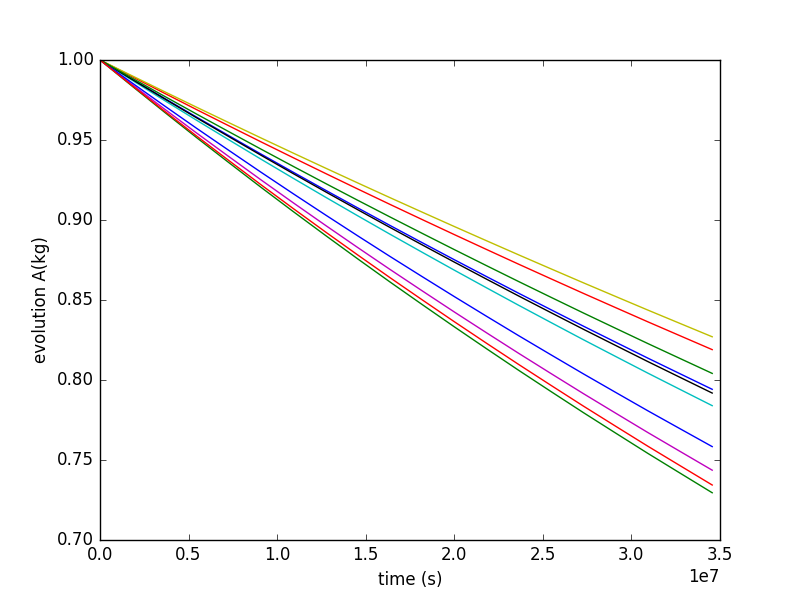
\includegraphics[scale=0.7]{../../tests/framework/user_guide/ravenTutorial/gold/ROMLoad/1-historyROMPlot_line.png}
  \caption{Plot of the histories generated by the Monte Carlo sampling of pickled ROM for variable $A$ (10 samples).}
  \label{fig:historiesROMPlotLine_A}
\end{figure}
%%%%%%%%%%%%%%%%%%%%%%%%%%%%%%%%%%%%%%%%%%%%%%%%%%%%%%%%%%

Finally, ROMs are generally not constructed for all possible inputs, geometries or representing all outputs. However,
it is possible to build a ROM of faster solution with respect to the original set. The accuracy in the prediction
can be obtained by further training. Figure~\ref{fig:romConstruction} shows the general workflow for ROM construction.

%%%%%%%%%%%%%%%%%%%%%%%%%%%%%%%%%%%%%%%%%%%%%%%%%%%%%%%%%%
%figure rom construction
\begin{figure}[h!]
  \centering
  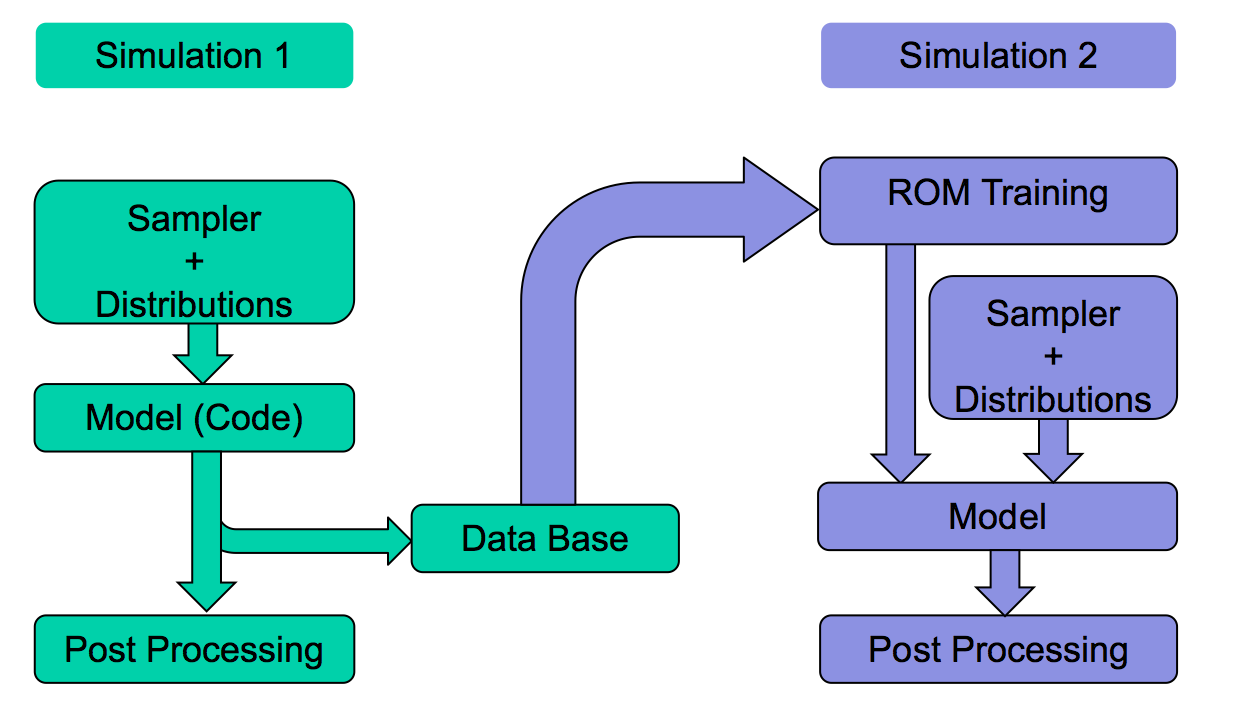
\includegraphics[scale=0.7]{./pics/romConstruction.png}
  \caption{Workflow for ROM construction}
  \label{fig:romConstruction}
\end{figure}
%%%%%%%%%%%%%%%%%%%%%%%%%%%%%%%%%%%%%%%%%%%%%%%%%%%%%%%%%%

\clearpage










% post-processors
\subsection{Build RAVEN Input: \xmlNode{PostProcess}}
\label{sub:ravenPostProcess}
The \textbf{PostProcess} step is used to post-process data or manipulate RAVEN entities. It is intended to perform
a single action that is employed by a \textbf{Model} of type \textbf{PostProcessor}. The specification of this
type of step is defined within a \xmlNode{PostProcess} XML block. As for the other objects, the attribute 
\xmlAttr{name} is required and is used to refer to this specific entity in the \xmlNode{RunInfo} block under
the \xmlNode{Sequence} node.

In the \xmlNode{PostProcess} input block, the user needs to specify the objects needed for the different allowable
roles. This step requires the following roles:

\begin{itemize}
  \item \xmlNode{Input}: accepts \textbf{Files}, \textbf{DataObjects} or \textbf{Databases}.
  \item \xmlNode{Model}: Only \xmlString{Models} and \xmlString{PostProcessor} can be assigned to the node's
    attributes \xmlAttr{class} and \xmlAttr{type}, respectively.
  \item \xmlNode{Output}: accepts \textbf{Files}, \textbf{DataObjects}, \textbf{Databases} or \textbf{OutStreams}.
\end{itemize}

As mentioned before, only the model with type \textbf{PostProcessor} is allowed for this step. A post-processor
can be considered as an action performed on a set of data or other type of objects. Most of the post-processors
contained in RAVEN, employ a mathematical operation on the data given as \textbf{``Input''}. Currently, the
following \textbf{PostProcessor} are available in RAVEN:

\begin{itemize}
  \itemsep0em
  \item \textbf{BasicStatistics}
  \item \textbf{ComparisonStatistics}
  \item \textbf{ImportanceRank}
  \item \textbf{SafestPoint}
  \item \textbf{LimitSurface}
  \item \textbf{LimitSurfaceIntegral}
  \item \textbf{External}
  \item \textbf{TopologicalDecomposition}
  \item \textbf{RavenOutput}
  \item \textbf{DataMining}
\end{itemize}

One can use the node attribute \xmlAttr{subType} to select which of the post-processors to be used. As with other
objects, the attribute \xmlAttr{name} is always required so that other RAVEN input XML blocks can use this name
to refer to this specific entity. In addition, each post-processor may require extra sub-nodes, and the user can refer
to the RAVEN user manual for the detailed specifications.

In this example, the \textbf{BasicStatistics} post-processor is used to demonstrate the \textbf{PostProcess} step.
\textbf{BasicStatistics} is a container of the algorithms to compute many of the most important statistical quantities.
Both \textbf{PointSet} and \textbf{HistorySet} can be accepted to compute the static statistics and dynamic statistics,
respectively. In case an \textbf{HistorySet} is provided as \textbf{Input}, the user need to define the \textbf{pivotParameter},
and sometimes the user need to synchronize the \textbf{HistorySet} first via the \textbf{Interfaced} post-processor of
type \textbf{HistorySetSync}.
\xmlExample{framework/user_guide/ravenTutorial/PostProcess.xml}{Models}
In this example, all the metrics of \textbf{BasicStatistics} will be computed for the response $A$.

The \xmlNode{Files} will be used to include all input and output files. In this example, a single input file
for the driven code and two output files of the \textbf{PostProcess} step are defined here. As shown in the following,
two output files are defined for this case study to store the static statistics and dynamic statistics information.
The \xmlString{time} is used as the \xmlNode{pivotParameter}.
\xmlExample{framework/user_guide/ravenTutorial/PostProcess.xml}{Files}


As before, all defined RAVEN entities are combined in the \xmlNode{Steps} block.
\xmlExample{framework/user_guide/ravenTutorial/PostProcess.xml}{Steps}
In this case, three steps have been defined:

\begin{itemize}
  \item \xmlNode{MultiRun} named ``sampleMC'', used to run the multiple instances of the driven code and
     collect the outputs in the two \textit{DataObjects}. As it can be seen, the \xmlNode{Sampler} is inputted
     to communicate to the \textit{Step} that the driven code needs to be perturbed through the Monte Carlo sampling
     strategy.
  \item \xmlNode{PostProcess} named ``statAnalysis\_1'', is used to compute all the statistical moments and FOMs
    based on the data obtained through the sampling strategy. As it can be noticed, the \xmlString{PointSet}
    ``samplesMC'' is used as input to compute the static statistics.
  \item \xmlNode{PostProcess} named ``statAnalysis\_2'', is used to compute all the statistical moments and FOMs
    based on the data obtained through the sampling strategy. As it can be noticed, the \xmlString{HistorySet}
    ``histories'' is used as input to compute the dynamic statistics.
\end{itemize}

%FIXME: The outputs from PostProcess is now stored in the DataObjects, XML format is not supported
%The results from the first \textbf{PostProcess} are listed as follows:
%\xmlExample{framework/user_guide/ravenTutorial/gold/stat/static.xml}{BasicStatisticsPP}


\section{Forward Sampling Strategies}
\label{sec:forwardSamplingStrategies}
In order to perform UQ and dynamic
probabilistic risk assessment (DPRA),
a sampling strategy needs to be employed. The sampling strategy
perturbs the input space (domain of the uncertainties) to explore
the response of a complex system in relation to selected FOMs.

The most widely used strategies to perform UQ and PRA are generally
collected in RAVEN as \textit{\textbf{Forward}} samplers. \textit{\textbf{Forward}} samplers include
all the strategies that simply perform the sampling of the input space.  These strategies sample
without exploiting, through learning approaches,
the information made available from the outcomes of evaluation previously performed (adaptive sampling) and the
common system evolution (patterns) that different sampled calculations can generate in the phase space (Dynamic Event Tree).

As mentioned in Section~\ref{sub:tutorialMultiRun}, RAVEN has
several different \textit{\textbf{Forward}} samplers:
\begin{itemize}
  \item \textit{Monte-Carlo}
  \item \textit{Grid-based}
  \item \textit{Stratified} and its specialization named \textit{Latin Hyper Cube}.
\end{itemize}
In addition, RAVEN posses advanced \textit{\textbf{Forward}} sampling strategies that:
\begin{itemize}
  \item Build a grid in the input space selecting evaluation points
    based on characteristic quadratures as part of stochastic collocation
    for generalized polynomial chaos method (\textit{Sparse
    Grid Collocation} sampler);
  \item Use high-density model reduction (HDMR) a.k.a. Sobol
    decomposition to approximate a function as the sum of
    interactions with increasing complexity (\textit{Sobol} sampler).
\end{itemize}
In the following subsections, we provide examples of input files
in RAVEN using the method, with explanatory commentary.
%%%%%%%%%%%%%%%%%%%%%%%%%
%%%%%%%%  MONTE-CARLO %%%%%%%%
%%%%%%%%%%%%%%%%%%%%%%%%%
\subsection{Monte-Carlo sampling through RAVEN}
\label{sub:MCexample}
The Monte-Carlo method is one of the most-used methodologies in several mathematic disciplines. In this section,
we will explain the techniques for employing this methodology in RAVEN, and we recommend the user to read the
theory manual to explore the theory of the method.
The goals of this section are about learning how to:
 \begin{enumerate}
   \item Set up a simple Monte-Carlo sampling for perturbing the input space of a driven code
   \item Load the outputs of the code into RAVEN DataObjects (HistorySets and PointSets)
   \item Print the contents of DataObjects to file
   \item Generate plots of the sampling results.
\end{enumerate}
In order to accomplish these tasks, the following RAVEN \textbf{Entities} (XML blocks in the RAVEN input file) are needed:
\begin{enumerate}
   \item \textbf{\textit{RunInfo}}:
     \xmlExample{framework/user_guide/ForwardSamplingStrategies/forwardSamplingMontecarlo.xml}{RunInfo}
     As discussed in Section~\ref{sub:singleRun}, the \textit{RunInfo} \textbf{Entity} sets up the analysis
     that the user wants to perform. In this specific case, two steps (\xmlNode{Sequence}) are sequentially run
     using 1 processor (\xmlNode{batchSize}). If this number change into 12, this means that
     12 instances of the driven code are run simultaneously. 
     Note that the \xmlNode{JobName} is not required, but is useful in identifying the input file.
   \item \textbf{\textit{Files}}:
     \xmlExample{framework/user_guide/ForwardSamplingStrategies/forwardSamplingMontecarlo.xml}{Files}
     Since the driven code uses a single input file, in this section the original input is identified and
     named. As detailed in the user manual, the attribute \xmlAttr{name} represents the alias that is used in
     all the other input blocks in order to refer to this file.
   \item \textbf{\textit{Models}}:
     \xmlExample{framework/user_guide/ForwardSamplingStrategies/forwardSamplingMontecarlo.xml}{Models}
     The Model used in this example is the
     \textbf{AnalyticalBateman} external model, which is defined in section \ref{sec:analyticalbateman}.  This model uses a keyword-based input file
     and exports its output file in a CSV format, so the \textit{GenericCode} interface is used.
   \item \textbf{\textit{Distributions}}:
     \xmlExample{framework/user_guide/ForwardSamplingStrategies/forwardSamplingMontecarlo.xml}{Distributions}
     In the \xmlNode{Distributions} block, the stochastic model for the uncertainties treated by the
     \xmlNode{Sampler} is defined. In this case two distributions are defined:
     \begin{itemize}
      \item $sigma \sim \mathbb{U}(1,10)$, used to model the uncertainties
        associated with the \textit{sigma} Model variables
      \item  $decayConstant \sim \mathbb{U}(0.5e-8,1e-8)$,  used to
        model the uncertainties associated with the Model variable \textit{decay constants}.  Note that the
        same distribution can be re-used for multiple input variables, while still keeping those variables
        independent.
     \end{itemize}
   \item \textbf{\textit{Samplers}}:
     \xmlExample{framework/user_guide/ForwardSamplingStrategies/forwardSamplingMontecarlo.xml}{Samplers}
      To employ the Monte-Carlo sampling strategy ($100$ samples), a
      \xmlNode{MonteCarlo} node needs to be defined.  The
      Monte-Carlo method is employed on $eight$ model variables, each of which are listed by name
      and are associated with a distribution.
      Note that all the \textit{decay-\*} and
      \textit{sigma-\*} variables are associated with the distributions
      $decayConstant$ and $sigma$, respectively.
   \item \textbf{\textit{DataObjects}}:
     \xmlExample{framework/user_guide/ForwardSamplingStrategies/forwardSamplingMontecarlo.xml}{DataObjects}
      In this block, two \textit{DataObjects} are defined to store results: 1) a PointSet named
      ``samples'', 2) a HistorySet named ``histories''.
      Note that in the \xmlNode{Input} node all the uncertainties
      perturbed through the Monte-Carlo strategy are listed. By this, any
      realization in the input space is linked in the DataObject to the outputs listed in the
      \xmlNode{Output} node.
   \item \textbf{\textit{OutStreams}}:
     \xmlExample{framework/user_guide/ForwardSamplingStrategies/forwardSamplingMontecarlo.xml}{OutStreams}
 %%%%%%%%%%%%%%%%%%%%%%%%%%%%%%%%%%%%%%%%%%%%%%%%%%%%%%%%%%
 %figure histories
 \begin{figure}[h!]
  \centering
  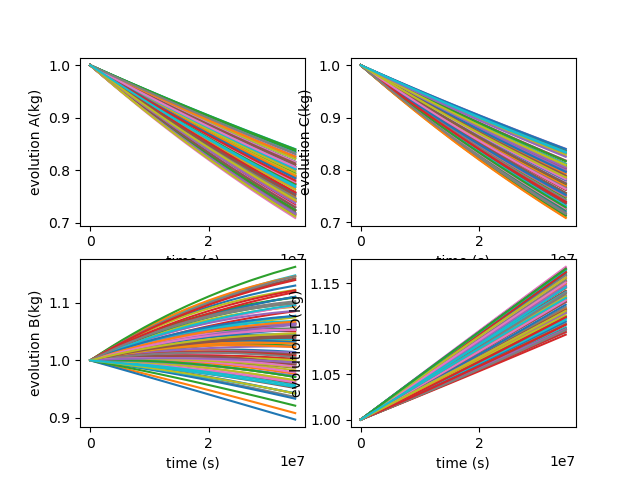
\includegraphics[scale=0.7]{../../tests/framework/user_guide/ForwardSamplingStrategies/gold/RunDir/MonteCarlo/1-historyPlot_line-line-line-line.png}
  \caption{Plot of the histories generated by the Monte Carlo sampling for variables $A,B,C,D$.}
  \label{fig:historiesMCPlotLine}
 \end{figure}
 %%%%%%%%%%%%%%%%%%%%%%%%%%%%%%%%%%%%%%%%%%%%%%%%%%%%%%%%%%
 To see the results of the simulation, \xmlNode{OutStreams} are included in the input.
  In this block, both OutStream types are used:
  \begin{itemize}
    \item \textit{Print}:
     \begin{itemize}
       \item ``samples'' connected with the \textit{DataObjects} \textbf{Entity} ``samples''
                (\xmlNode{source})
       \item ``histories'' connected with the \textit{DataObjects} \textbf{Entity} ``histories'' (\xmlNode{source})
     \end{itemize}
     Note that in RAVEN, multiple entities can have the same name, as it takes a class, a type, and a name to
     uniquely identify a RAVEN object.
      When the two OutStream objects are used, all the information contained in the
      linked \textit{DataObjects} are going
    to be exported in CSV files (\xmlNode{type}).
    \item \textit{Plot}:
    \begin{itemize}
      \item ``historiesPlot'' connected with the  \textit{DataObjects}
      \textbf{Entity} ``samples''.  This plot will draw the final state of the
      variables $A,B,C,D$ with respect to the input variables $sigma$(s)
      and $decay$(s) .
      \item ``samplesPlot3D'' connected with the
      \textit{DataObjects} \textbf{Entity} ``histories''. This plot will draw the
      evolution of the variables $A,B,C,D$.
    \end{itemize}
     Note that both plots use gridded subplots. Four plots
     are placed in each of the figures.
  \end{itemize}
   \item \textbf{\textit{Steps}}:
     \xmlExample{framework/user_guide/ForwardSamplingStrategies/forwardSamplingMontecarlo.xml}{Steps}
 %%%%%%%%%%%%%%%%%%%%%%%%%%%%%%%%%%%%%%%%%%%%%%%%%%%%%%%%%%
 %figure samples
 \begin{figure}[h!]
  \centering
  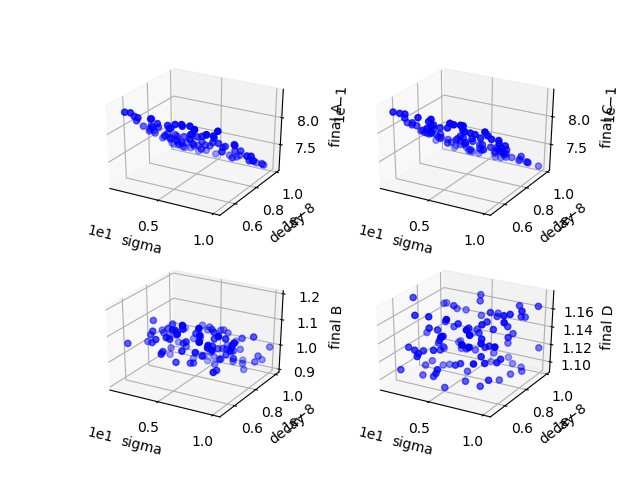
\includegraphics[scale=0.7]{../../tests/framework/user_guide/ForwardSamplingStrategies/gold/RunDir/MonteCarlo/1-samplesPlot3D_scatter-scatter-scatter-scatter.png}
  \caption{Plot of the samples generated by the MC sampling for variables $A,B,C,D$.}
  \label{fig:samplesMCPlotLine}
 \end{figure}
 %%%%%%%%%%%%%%%%%%%%%%%%%%%%%%%%%%%%%%%%%%%%%%%%%%%%%%%%%%
   Once all the other entities are defined in the RAVEN input file, they must be combined in the
   \xmlNode{Steps} block, which dictates the workflow of RAVEN.  For this case,
   two \xmlNode{Steps} are defined:
   \begin{itemize}
     \item \xmlNode{MultiRun} ``sample'', used to run the multiple
     instances of the driven code and
     collect the outputs in the two \textit{DataObjects}. As it can be
     seen, the \xmlNode{Sampler} is specified to communicate to the
     \textit{Step} that the driven code needs to
     be perturbed through the Monte-Carlo sampling.
     \item  \xmlNode{IOStep} named ``writeHistories'', used to 1) dump
     the ``histories'' and ``samples'' \textit{DataObjects}
     \textbf{Entity} to a CSV file and 2) plot the data in the EPS file.
   \end{itemize}
\end{enumerate}
 Figures~\ref{fig:historiesMCPlotLine} and ~\ref{fig:samplesMCPlotLine} show the report
 generated by RAVEN of the evolution of the
 variables $A,B,C,D$ and their final values, respectively.
%%%%%%%%%%%%%%%%%%%%%%%%%
%%%%%%%%          GRID          %%%%%%%%
%%%%%%%%%%%%%%%%%%%%%%%%%
\subsection{Grid sampling through RAVEN}
\label{sub:Gridexample}
The Grid sampling method (also known as Full Factorial Design of Experiment) represents one of the simplest methodologies that can be employed in order to explore the interaction of multiple random variables with respect
selected FOMs.
The goal of this section is to show how to:
 \begin{enumerate}
   \item Set up a simple Grid sampling for performing a parametric analysis of a driven code
   \item Load the outputs of the code into the RAVEN DataObjects system
   \item Print out what contained in the DataObjects
   \item Generate basic plots of the code result.
\end{enumerate}
In order to accomplish these tasks, the following RAVEN \textbf{Entities} (XML blocks in the input files) are required:
\begin{enumerate}
   \item \textbf{\textit{RunInfo}}:
     \xmlExample{framework/user_guide/ForwardSamplingStrategies/forwardSamplingGrid.xml}{RunInfo}
   As shown in Section~\ref{sub:singleRun}, the \textit{RunInfo} \textbf{Entity} is intended to set up the desired analysis.
   In this specific case, two steps (\xmlNode{Sequence}) are sequentially run
   using 2 processors (\xmlNode{batchSize}). This means that
   2 instances of the driven code are  run simultaneously.
   \item \textbf{\textit{Files}}:
     \xmlExample{framework/user_guide/ForwardSamplingStrategies/forwardSamplingGrid.xml}{Files}
   Since the driven code uses a single input file, in this section the original input is placed. As described in the user manual~\cite{RAVENuserManual}
   the attribute  \xmlAttr{name} represents the alias that is used in all the other input blocks in order to refer to this file.
   \item \textbf{\textit{Models}}:
     \xmlExample{framework/user_guide/ForwardSamplingStrategies/forwardSamplingGrid.xml}{Models}
 The Model here is represented by the
 \textbf{AnalyticalBateman}, which already dumps its output file in a
 CSV format (standard format that RAVEN can read). For this reason,
 the \textit{GenericCode} interface is used.
   \item \textbf{\textit{Distributions}}:
     \xmlExample{framework/user_guide/ForwardSamplingStrategies/forwardSamplingGrid.xml}{Distributions}
  In the Distributions XML section, the stochastic model for the
  uncertainties  treated by the Grid sampling are reported. In
  this case two distributions are defined:
  \begin{itemize}
    \item $sigma \sim \mathbb{U}(1,10)$, used to model the uncertainties
    associated with  the Model \textit{sigma}(s)
    \item  $decayConstant \sim \mathbb{U}(0.5e-8,1e-8)$,  used to
    model the uncertainties
    associated with  the Model \textit{decay constants}.
  \end{itemize}
   \item \textbf{\textit{Samplers}}:
     \xmlExample{framework/user_guide/ForwardSamplingStrategies/forwardSamplingGrid.xml}{Samplers}
  To employ the Grid sampling strategy, a
  \xmlNode{Grid} node needs to be specified. As shown above, in each variable section, the  \xmlNode{grid} is defined.
  The number of samples finally requested are equal to $n_{samples} = \prod_{i=1}^{n} (n_{steps_{i}} +1)= 256$.
  Note that, for each variable, can be defined either in probability (CDF) or in absolute value.
   \item \textbf{\textit{DataObjects}}:
     \xmlExample{framework/user_guide/ForwardSamplingStrategies/forwardSamplingGrid.xml}{DataObjects}
  Int this block, two \textit{DataObjects} are defined: 1) PointSet named
  ``samples'', and 2) HistorySet named ``histories''.
  In the \xmlNode{Input} node all the variables
  perturbed through the Grid strategy are listed. In this way, any
  realization in the input space is linked to the outputs listed in  the
  \xmlNode{Output} node.
   \item \textbf{\textit{OutStreams}}:
     \xmlExample{framework/user_guide/ForwardSamplingStrategies/forwardSamplingGrid.xml}{OutStreams}
 %%%%%%%%%%%%%%%%%%%%%%%%%%%%%%%%%%%%%%%%%%%%%%%%%%%%%%%%%%
 %figure histories
 \begin{figure}[h!]
  \centering
  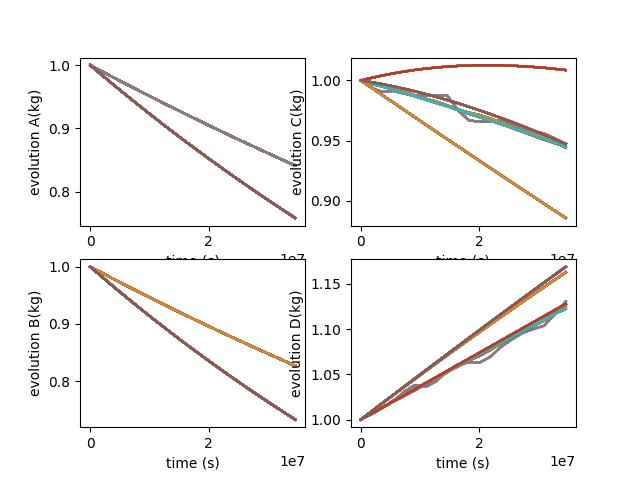
\includegraphics[scale=0.7]{../../tests/framework/user_guide/ForwardSamplingStrategies/gold/RunDir/Grid/1-historyPlot_line-line-line-line.png}
  \caption{Plot of the histories generated by the Grid sampling for variables $A,B,C,D$.}
  \label{fig:historiesGridPlotLine}
 \end{figure}
 %%%%%%%%%%%%%%%%%%%%%%%%%%%%%%%%%%%%%%%%%%%%%%%%%%%%%%%%%%
  In this block, both the Out-Stream types are constructed:
  \begin{itemize}
    \item \textit{Print}:
     \begin{itemize}
       \item named ``samples'' connected with the \textit{DataObjects} \textbf{Entity} ``samples''
                (\xmlNode{source})
       \item named ``histories'' connected with the \textit{DataObjects} \textbf{Entity} ``histories'' (\xmlNode{source}).
     \end{itemize}
      When these objects get used, all the information contained in the
      linked  \textit{DataObjects} are going
    to be exported in CSV files (\xmlNode{type}).
    \item \textit{Plot}:
    \begin{itemize}
      \item named ``historiesPlot'' connected with the  \textit{DataObjects}
      \textbf{Entity} ``samples''.  This plot will draw the final state of the
      variables $A,B,C,D$ with respect to the input variables $sigma$(s)
      and $decay$(s).
      \item named ``samplesPlot3D'' connected with the
      \textit{DataObjects} \textbf{Entity} ``histories''. This plot will draw the
      evolution of the variables $A,B,C,D$.
    \end{itemize}
     As it can be noticed, both plots are of type \textit{SubPlot}. Four plots
     are placed in each of the figures.
  \end{itemize}
   \item \textbf{\textit{Steps}}:
     \xmlExample{framework/user_guide/ForwardSamplingStrategies/forwardSamplingGrid.xml}{Steps}
 %%%%%%%%%%%%%%%%%%%%%%%%%%%%%%%%%%%%%%%%%%%%%%%%%%%%%%%%%%
 %figure samples
 \begin{figure}[h!]
  \centering
  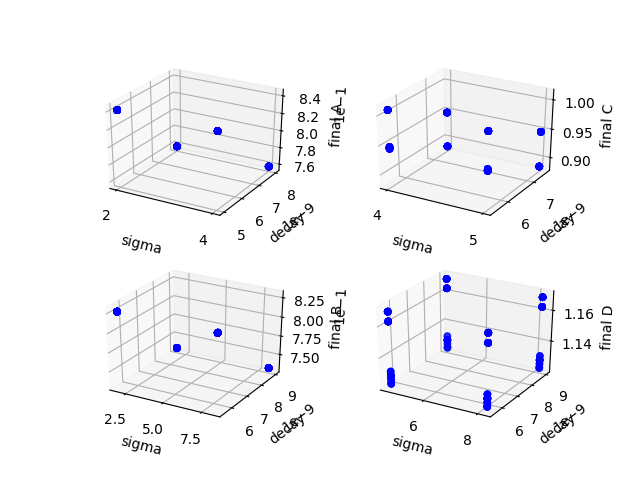
\includegraphics[scale=0.7]{../../tests/framework/user_guide/ForwardSamplingStrategies/gold/RunDir/Grid/1-samplesPlot3D_scatter-scatter-scatter-scatter.png}
  \caption{Plot of the samples generated by the Grid sampling for variables $A,B,C,D$.}
  \label{fig:samplesGridPlotLine}
 \end{figure}
 %%%%%%%%%%%%%%%%%%%%%%%%%%%%%%%%%%%%%%%%%%%%%%%%%%%%%%%%%%
   Finally, all the previously defined \textbf{Entities} can be combined in
   the \xmlNode{Steps} block. As inferable,
   two \xmlNode{Steps} have been inputted:
   \begin{itemize}
     \item \xmlNode{MultiRun} named ``sample'', is used to run the multiple
     instances of the code and
     collect the outputs in the two \textit{DataObjects}. As it can be
     seen, the \xmlNode{Sampler} is inputted to communicate to the
     \textit{Step} that the driven code needs to
     be perturbed through the Grid sampling
     \item  \xmlNode{IOStep} named ``writeHistories'', used to 1) dump
     the ``histories'' and ``samples'' \textit{DataObjects}
     \textbf{Entity} in a CSV file and 2) plot the data in the PNG file and
     on the screen.
   \end{itemize}
\end{enumerate}
 Figures~\ref{fig:historiesGridPlotLine} and ~\ref{fig:samplesGridPlotLine}  report the evolution of the
 variables $A,B,C,D$ and their final values, respectively.

%%%%%%%%%%%%%%%%%%%%%%%%%
%%%%%%%%    STRATIFIED    %%%%%%%%
%%%%%%%%%%%%%%%%%%%%%%%%%
\subsection{Stratified sampling through RAVEN}
\label{sub:Stratifiedexample}
The Stratified sampling is a class of methods that relies on the assumption that the input space (i.e.,uncertainties)
can be separated in regions (strata) based on similarity of the response of the system for input set within the
same strata. Following this assumption, the most rewarding (in terms of computational cost vs. knowledge gain)
sampling strategy would be to place one sample for each region. In this way, the same information is not
collected more than once and all the prototypical behavior are sampled at least once. In
Figure~\ref{fig:StratifiedSamplingExample}, the Stratified sampling approach is exemplified.
 \begin{figure}[h!]
  \centering
  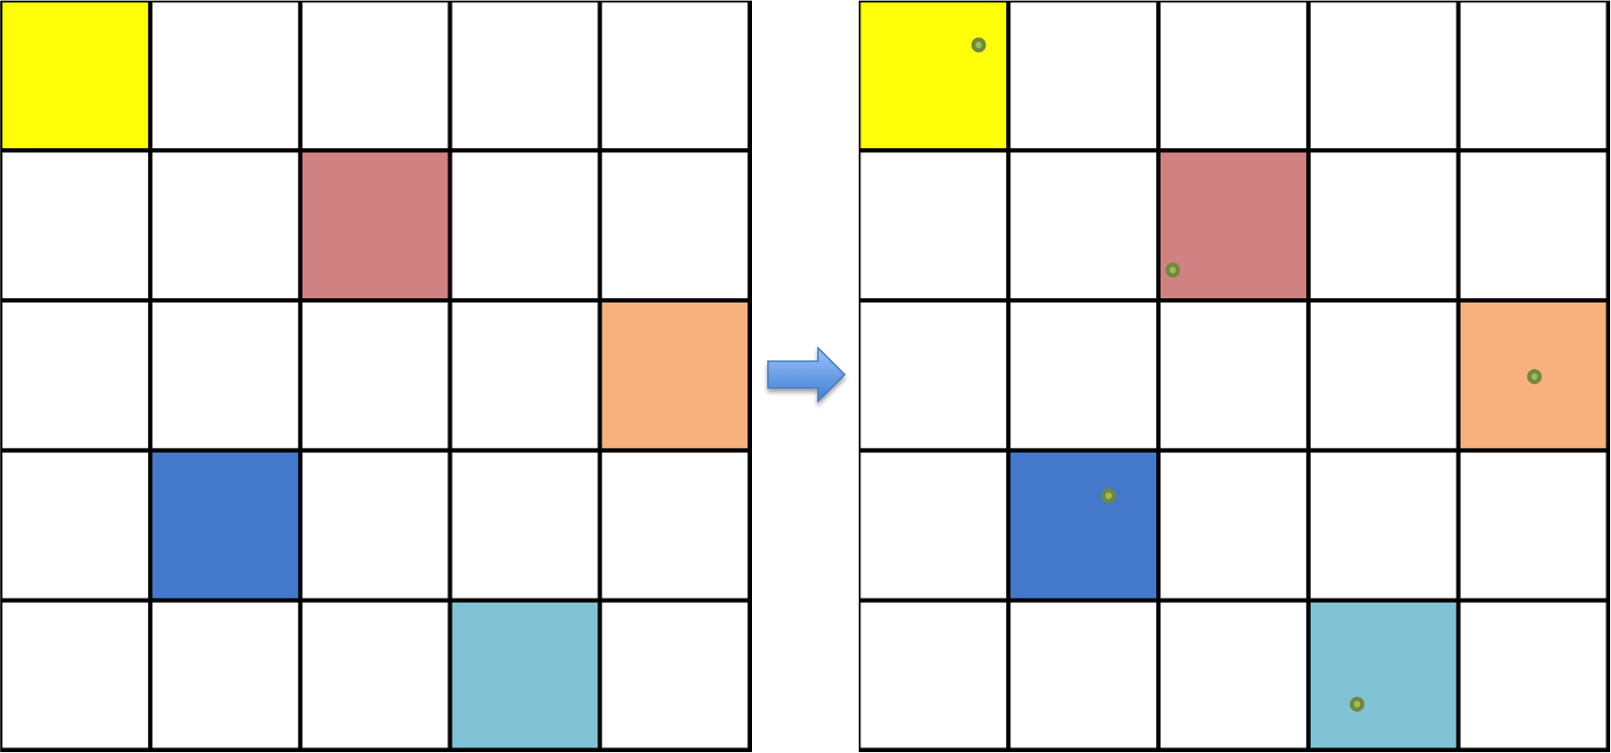
\includegraphics[scale=0.55]{pics/StratifiedSamplingExample.png}
  \caption{Example of Stratified sampling approach.}
  \label{fig:StratifiedSamplingExample}
 \end{figure}
\\The goal of this section is to show how to:
 \begin{enumerate}
   \item Set up a simple Stratified sampling in order to perform a parametric analysis on a driven code
   \item Load the outputs of the code into the RAVEN DataObjects system
   \item Print out what contained in the DataObjects
   \item Generate basic plots of the code result.
\end{enumerate}
To accomplish these tasks, the following RAVEN \textbf{Entities} (XML blocks in the input files) are defined:
\begin{enumerate}
   \item \textbf{\textit{RunInfo}}:
     \xmlExample{framework/user_guide/ForwardSamplingStrategies/forwardSamplingStratified.xml}{RunInfo}
   As reported in Section~\ref{sub:singleRun}, the \textit{RunInfo} \textbf{Entity} is intended to set up the analysis
   that the user wants to perform. In this specific case, two steps (\xmlNode{Sequence}) are  run
   using 1 processor (\xmlNode{batchSize}). This means that
   1 instance of the driven code are run simultaneously.
   \item \textbf{\textit{Files}}:
     \xmlExample{framework/user_guide/ForwardSamplingStrategies/forwardSamplingStratified.xml}{Files}
   Since the considered code uses a single input file, in this section the original input is placed.
   The attribute  \xmlAttr{name} represents the alias that is going to be used in all the other input blocks in order to refer to this file.
   \item \textbf{\textit{Models}}:
     \xmlExample{framework/user_guide/ForwardSamplingStrategies/forwardSamplingStratified.xml}{Models}
 The Model here is represented by the
 \textbf{AnalyticalBateman}, which already dumps its output file in a
 CSV format (standard format that RAVEN can read). For this reason,
 the \textit{GenericCode} interface is used.
   \item \textbf{\textit{Distributions}}:
     \xmlExample{framework/user_guide/ForwardSamplingStrategies/forwardSamplingStratified.xml}{Distributions}
  In the Distributions XML section, the stochastic model for the
  uncertainties  treated by the Stratified sampling are reported. In
  this case two distributions are defined:
  \begin{itemize}
    \item $sigma \sim \mathbb{U}(1,10)$, used to model the uncertainties
    associated with  the Model \textit{sigma}(s)
    \item  $decayConstant \sim \mathbb{U}(0.5e-8,1e-8)$,  used to
    model the uncertainties
    associated with  the Model \textit{decay constants}.
  \end{itemize}
   \item \textbf{\textit{Samplers}}:
     \xmlExample{framework/user_guide/ForwardSamplingStrategies/forwardSamplingStratified.xml}{Samplers}
  To employ the Stratified sampling strategy, a
  \xmlNode{Stratified} node needs to be specified. In each variable section, the  \xmlNode{grid} is defined.
  It is important to mention that the number of \xmlAttr{steps} needs to be the same for each of the variables,
  since, as reported in previous section, the Stratified sampling strategy it discretizes the domain in strata.
  The number of samples finally requested is equal to $n_{samples} = n_{steps} = 100$.
  If the grid for each variables is defined in CDF and of  \xmlAttr{type} = ``equal'', the Stratified
  sampling corresponds to the well-known Latin Hyper Cube sampling.
   \item \textbf{\textit{DataObjects}}:
     \xmlExample{framework/user_guide/ForwardSamplingStrategies/forwardSamplingStratified.xml}{DataObjects}
  In this block, two \textit{DataObjects} are defined: 1) PointSet named
  ``samples'', 2) HistorySet named ``histories''.
  In the \xmlNode{Input} node all the variables
  perturbed through the Stratified strategy are listed. In this way, any
  realization in the input space is linked to the outputs listed in  the
  \xmlNode{Output} node.
   \item \textbf{\textit{OutStreams}}:
     \xmlExample{framework/user_guide/ForwardSamplingStrategies/forwardSamplingStratified.xml}{OutStreams}
 %%%%%%%%%%%%%%%%%%%%%%%%%%%%%%%%%%%%%%%%%%%%%%%%%%%%%%%%%%
 %figure histories
 \begin{figure}[h!]
  \centering
  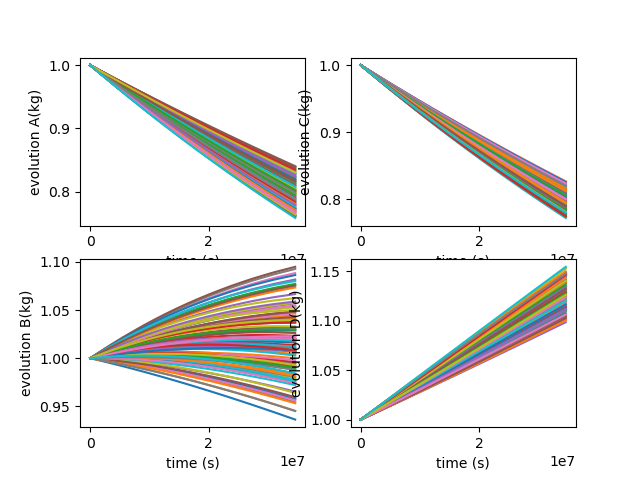
\includegraphics[scale=0.7]{../../tests/framework/user_guide/ForwardSamplingStrategies/gold/RunDir/Stratified/1-historyPlot_line-line-line-line.png}
  \caption{Plot of the histories generated by the Stratified sampling for variables $A,B,C,D$.}
  \label{fig:historiesStratifiedPlotLine}
 \end{figure}
 %%%%%%%%%%%%%%%%%%%%%%%%%%%%%%%%%%%%%%%%%%%%%%%%%%%%%%%%%%
  In this block, both the Out-Stream types are constructed:
  \begin{itemize}
    \item \textit{Print}:
     \begin{itemize}
       \item named ``samples'' connected with the \textit{DataObjects} \textbf{Entity} ``samples''
                (\xmlNode{source})
       \item named ``histories'' connected with the \textit{DataObjects} \textbf{Entity} ``histories'' (\xmlNode{source}).
     \end{itemize}
      When these objects get used, all the information contained in the
      linked  \textit{DataObjects} are going
    to be exported in CSV files (\xmlNode{type}).
    \item \textit{Plot}:
    \begin{itemize}
      \item named ``historiesPlot'' connected with the  \textit{DataObjects}
      \textbf{Entity} ``samples''.  This plot will draw the final state of the
      variables $A,B,C,D$ with respect to the input variables $sigma$(s)
      and $decay$(s)
      \item named ``samplesPlot3D'' connected with the
      \textit{DataObjects} \textbf{Entity} ``histories''. This plot will draw the
      evolution of the variables $A,B,C,D$.
    \end{itemize}
     As it can be noticed, both plots are of type \textit{SubPlot}. Four plots
     are going to be placed in each of the figures.
  \end{itemize}
   \item \textbf{\textit{Steps}}:
     \xmlExample{framework/user_guide/ForwardSamplingStrategies/forwardSamplingStratified.xml}{Steps}
 %%%%%%%%%%%%%%%%%%%%%%%%%%%%%%%%%%%%%%%%%%%%%%%%%%%%%%%%%%
 %figure samples
 \begin{figure}[h!]
  \centering
  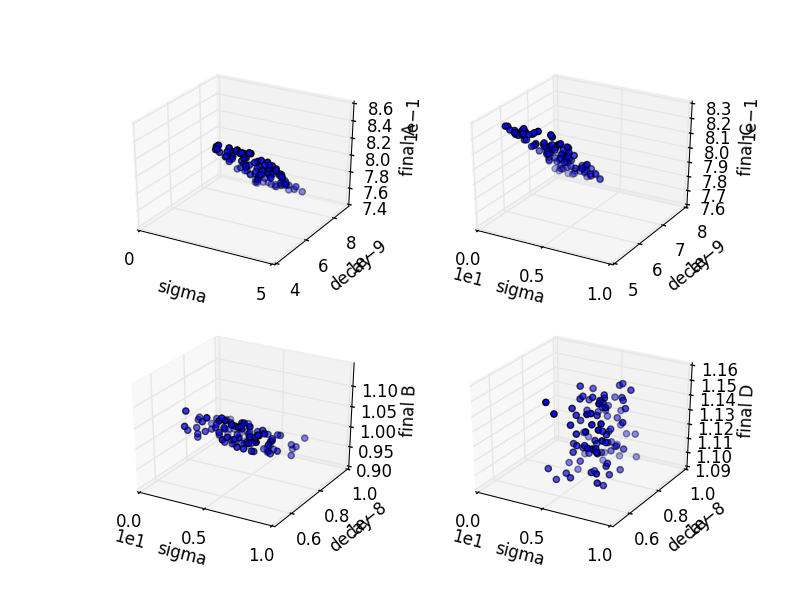
\includegraphics[scale=0.7]{../../tests/framework/user_guide/ForwardSamplingStrategies/gold/RunDir/Stratified/1-samplesPlot3D_scatter-scatter-scatter-scatter.png}
  \caption{Plot of the samples generated by the Stratified sampling for variables $A,B,C,D$.}
  \label{fig:samplesStratifiedPlotLine}
 \end{figure}
 %%%%%%%%%%%%%%%%%%%%%%%%%%%%%%%%%%%%%%%%%%%%%%%%%%%%%%%%%%
   Finally, all the previously defined \textbf{Entities} can be combined in
   the \xmlNode{Steps} block. As inferable,
   two \xmlNode{Steps} have been inputted:
   \begin{itemize}
     \item \xmlNode{MultiRun} named ``sample'', used to run the multiple
     instances of the driven code and
     collect the outputs in the two \textit{DataObjects}. As it can be
     seen, the \xmlNode{Sampler} is inputted to communicate to the
     \textit{Step} that the driven code needs to
     be perturbed through the Stratified sampling.
     \item  \xmlNode{IOStep} named ``writeHistories'', used to 1) dump
     the ``histories'' and ``samples'' \textit{DataObjects}
     \textbf{Entity} in a CSV file and 2) plot the data in the PNG file and
     on the screen.
   \end{itemize}
\end{enumerate}
 As previously mentioned, Figures~\ref{fig:historiesStratifiedPlotLine} and ~\ref{fig:samplesStratifiedPlotLine}  report the evolution of the
 variables $A,B,C,D$ and their final values, respectively.

%%%%%%%%%%%%%%%%%%%%%%%%%

\subsection{Sparse Grid Collocation sampling through RAVEN}
\label{sub:SGcsamplingExample}
The Sparse Grid Collocation sampler represents an advanced methodology to perform Uncertainty Quantification. They aim
to explore the input space leveraging the information contained in the associated probability density functions. It builds on generic Grid sampling by selecting evaluation points based on characteristic quadratures as part of stochastic collocation for generalized polynomial chaos uncertainty quantification. In collocation an N-D grid is constructed, with each uncertain variable providing an axis. Along each axis, the points of evaluation correspond to quadrature points necessary to integrate polynomials. In the simplest (and most naive) case, a N-D tensor product of all possible combinations of points from each dimension’s quadrature is constructed as sampling points. The number of necessary samples can be reduced by employing Smolyak-like sparse grid algorithms, which use reduced combinations of polynomial orders to reduce the necessary sampling space.
\\The goals of this section are about learning how to:
 \begin{enumerate}
   \item Set up a Sparse Grid Collocation sampling for the construction of a suitable surrogate model of a driven code
   \item Construct a GaussPolynomialRom surrogate model (training stage)
   \item Use the constructed GaussPolynomialRom surrogate model instead of the driven code.
\end{enumerate}
To accomplish these tasks, the following RAVEN \textbf{Entities} (XML blocks in the input files) need to be defined:
\begin{enumerate}
   \item \textbf{\textit{RunInfo}}:
     \xmlExample{framework/user_guide/ForwardSamplingStrategies/forwardSamplingSparseGrid.xml}{RunInfo}
   As reported in section~\ref{sub:singleRun}, the \textit{RunInfo} \textbf{Entity} is intended to set up the analysis
   that the user wants to perform. In this specific case, six steps (\xmlNode{Sequence}) are going to be sequentially run
   using twelve processors (\xmlNode{batchSize}).  The first two steps build the ROM
   (\xmlString{sample}, \xmlString{train}), the next two validate
   the ROM against the original Code Model (\xmlString{validateModel}, \xmlString{validateROM}),
   and the last two produce plots and print data (\xmlString{output\_print}, \xmlString{output\_plot}).
   \item \textbf{\textit{Files}}:
     \xmlExample{framework/user_guide/ForwardSamplingStrategies/forwardSamplingSparseGrid.xml}{Files}
   Since the driven code uses a single input file, in this section the original input is placed. As detailed in the user manual
   the attribute  \xmlAttr{name} represents the alias that is going to be used in all the other input blocks in order to refer to this file.
   \item \textbf{\textit{Models}}:
     \xmlExample{framework/user_guide/ForwardSamplingStrategies/forwardSamplingSparseGrid.xml}{Models}
 The goal of this example is the generation of a \text{GaussPolynomialRom}
 for subsequent usage instead of the original code.  In addition to the previously explained Code model,
 the ROM of type \textit{GaussPolynomialRom} is specified here. The ROM is generated through a Sparse Grid
 Collocation sampling strategy. All 4 targets $A,B,C,D$ are modeled through this ROM as function
 of the uncertain $sigma$ and $decay$ parameters.  Note that the \xmlNode{Interpolation} nodes are not
 required, but are included for the sake of demonstration.
   \item \textbf{\textit{Distributions}}:
     \xmlExample{framework/user_guide/ForwardSamplingStrategies/forwardSamplingSparseGrid.xml}{Distributions}
  In the Distributions XML section, the stochastic model for the
  uncertainties  treated by the Sparse Grid Collocation sampling are reported. In
  this case eight distributions are defined:
  \begin{itemize}
    \item $sigmaA \sim \mathbb{U}(6.9,8.1)$, used to model the uncertainty
    associated with  the Model \textit{sigma-A}
    \item $sigmaB \sim \mathbb{U}(3.9,5.1)$, used to model the uncertainty
    associated with  the Model \textit{sigma-B}
    \item $sigmaC \sim \mathbb{U}(1.9,3.1)$, used to model the uncertainty
    associated with  the Model \textit{sigma-C}
    \item $sigmaD \sim \mathbb{U}(0.9,1.1)$, used to model the uncertainty
    associated with  the Model \textit{sigma-D}
    \item  $decayConstantA \sim \mathbb{U}(3.8e-9,5.2e-9)$,  used to
    model the uncertainty
    associated with  the Model \textit{decay-A}
    \item  $decayConstantB \sim \mathbb{U}(5.8e-9,7.2e-9)$,  used to
    model the uncertainty
    associated with  the Model \textit{decay-B}
    \item  $decayConstantC \sim \mathbb{U}(6.8e-9,8.2e-9)$,  used to
    model the uncertainty
    associated with  the Model \textit{decay-C}
    \item  $decayConstantD \sim \mathbb{U}(7.8e-9,9.2e-9)$,  used to
    model the uncertainty
    associated with  the Model \textit{decay-D}.
  \end{itemize}
   \item \textbf{\textit{Samplers}}:
     \xmlExample[rom,ROM,SparseGridCollocation,MonteCarlo]{framework/user_guide/ForwardSamplingStrategies/forwardSamplingSparseGrid.xml}{Samplers}
  In order to employ the Sparse Grid Collocation sampling strategy, a
  \xmlNode{SparseGridCollocation} node needs to be defined.
  As can be
  seen from above, each variable is associated with a different distribution,
  defined in the  \xmlNode{Distributions} block.
  In addition, the \textit{GaussPolynomialRom} \xmlNode{ROM} is linked to the \xmlNode{SparseGridCollocation}
  sampler.  Because this sampler is used exclusively to build the ROM, some of the parameters of the ROM are
  needed by the sampler, and this connection makes that communication possible.  The setting of this ROM
  (e.g. polynomial order, Index set method, etc.) determines how the Stochastic Collocation Method is
  employed.

  Additionally, a \xmlNode{MonteCarlo} sampler is set up for validating the ROM against the original Code.  The random
  number generation seed (\xmlNode{initialSeed}) is specified and set to reset on each use
  (\xmlNode{reseedEachIteration}) so that the Monte Carlo sampler can be used to compare the ROM against the
  original model.  We use twenty samples (\xmlNode{limit}) to sample the ROM and the model, and then print and
  plot both data sets to compare them.
   \item \textbf{\textit{DataObjects}}:
     \xmlExample[rom,SparseGridCollocation]{framework/user_guide/ForwardSamplingStrategies/forwardSamplingSparseGrid.xml}{DataObjects}
  In this block, four \textit{DataObjects} are defined:
  1) a PointSet named ``inputPlaceholder'' used as a placeholder input for the ROM sampling step,
  2) a HistorySet named ``histories'' used to collect the samples needed to train the ROM,
  3) a PointSet named ``samplesModel'' to store the Code responses from Monte Carlo samples, and
  4) a PointSet named ``samplesROM'' to store the ROM responses from Monte Carlo samples.
 %%%%%%%%%%%%%%%%%%%%%%%%%%%%%%%%%%%%%%%%%%%%%%%%%%%%%%%%%%
 %%%%%%%%%%%%%%%%%%%%%%%%%%%%%%%%%%%%%%%%%%%%%%%%%%%%%%%%%%
 %figure histories
 \begin{figure}[h!]
  \centering
  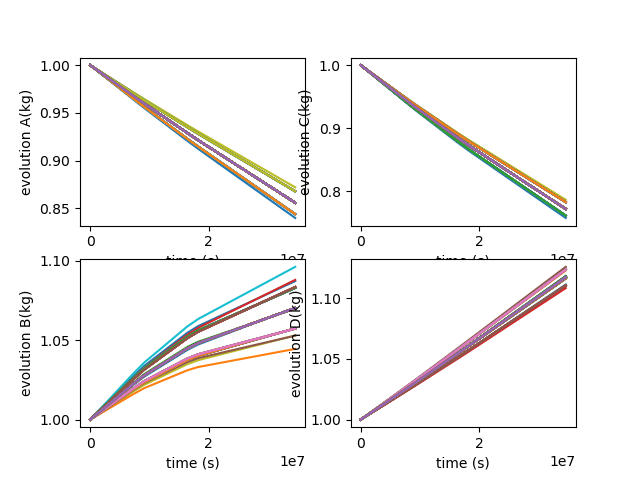
\includegraphics[scale=0.7]{../../tests/framework/user_guide/ForwardSamplingStrategies/gold/RunDir/SparseGrid/1-historyPlot_line-line-line-line.png}
  \caption{Plot of the training samples generated by the SparseGridCollocation sampling for variables $A,B,C,D$.}
  \label{fig:historiesSparseGridPlotLine}
 \end{figure}
 %%%%%%%%%%%%%%%%%%%%%%%%%%%%%%%%%%%%%%%%%%%%%%%%%%%%%%%%%%
 %%%%%%%%%%%%%%%%%%%%%%%%%%%%%%%%%%%%%%%%%%%%%%%%%%%%%%%%%%
   \item \textbf{\textit{OutStreams}}:
     \xmlExample{framework/user_guide/ForwardSamplingStrategies/forwardSamplingSparseGrid.xml}{OutStreams}
  In this block, the following Out-Stream types are constructed:
  \begin{itemize}
    \item \textit{Print}:
     \begin{itemize}
       \item named ``samplesModel'' connected with the \textit{DataObjects} \textbf{Entity} ``samplesModel''
                (\xmlNode{source})
       \item named ``samplesROM'' connected with the \textit{DataObjects} \textbf{Entity} ``samplesROM''
                (\xmlNode{source})
       \item named ``histories'' connected with the \textit{DataObjects} \textbf{Entity} ``histories'' (\xmlNode{source})
       \item named ``rom\_output'' connected with the \textit{ROM} \textbf{Entity} ``rom'' (\xmlNode{source}).
     \end{itemize}
      When these objects get used, all the information contained in the
      linked  \textit{DataObjects} are going
    to be exported in ether CSV files for DataObjects or XML files for ROMs (\xmlNode{type}).
    \item \textit{Plot}:
    \begin{itemize}
      \item named ``historyPlot'' connected with the  \textit{DataObjects}
      \textbf{Entity} ``histories''.  This plot will draw the time-dependent state of the
      variables $A,B,C,D$ with respect to the input variables $sigma$(s)
      and $decay$(s)
      \item named ``samplesModelPlot3D'' connected with the
      \textit{DataObjects} \textbf{Entity} ``samplesModel''. This plot will draw the
      variables $A,B,C,D$ as Monte Carlo sampled on the Code.
      \item named ``samplesROMPlot3D'' connected with the
      \textit{DataObjects} \textbf{Entity} ``samplesROM''. This plot will draw the
      variables $A,B,C,D$ as Monte Carlo sampled on the ROM.
    \end{itemize}
     As it can be noticed, both plots are of type \textit{SubPlot}. Four plots
     are going to be placed in each of the figures.
  \end{itemize}
   \item \textbf{\textit{Steps}}:
     \xmlExample[rom,SparseGridCollocation]{framework/user_guide/ForwardSamplingStrategies/forwardSamplingSparseGrid.xml}{Steps}
  %%%%%%%%%%%%%%%%%%%%%%%%%%%%%%%%%%%%%%%%%%%%%%%%%%%%%%%%%%
 %figure samples
 \begin{figure}[h!]
  \centering
  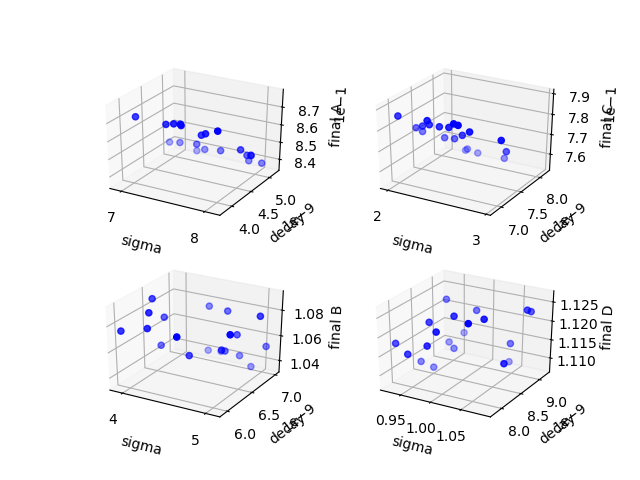
\includegraphics[scale=0.7]{../../tests/framework/user_guide/ForwardSamplingStrategies/gold/RunDir/SparseGrid/1-samplesModelPlot3D_scatter-scatter-scatter-scatter.png}
  \caption{Plot of validation samples generated by Monte Carlo sampling on the Code for variables $A,B,C,D$.}
  \label{fig:samplesSparseGridPlotModel}
 \end{figure}
 %%%%%%%%%%%%%%%%%%%%%%%%%%%%%%%%%%%%%%%%%%%%%%%%%%%%%%%%%%
   Finally, the previously defined \textbf{Entities} can be combined in
   the \xmlNode{Steps} block.
   The following \xmlNode{Steps} have been defined:
   \begin{itemize}
     \item \xmlNode{MultiRun} named ``sample'', used to run the training
     samples of the driven code and
     collect the outputs in the \textit{DataObjects}.
     The \xmlNode{Sampler} is specified to communicate to the
     \textit{Step} that the driven code needs to
     be sampled through the Sparse Grid Collocation sampling strategy;
     \item \xmlNode{RomTrainer} named ``train'', used to train (i.e.,
     construct) the GaussPolynomial ROM. This step is essential if the
     user want to use the ROM in later steps;
     \item \xmlNode{MultiRun} named ``sampleModel'', used to run the
     Monte Carlo perturbed samples of the original Model for use in verification.  The results are
     collected in the \textit{samplesModel} \textit{DataObjects}.
     \item \xmlNode{MultiRun} named ``sampleROM'', used to run the
     Monte Carlo perturbed samples of the previously constructed ROM for use in verificaiton.  The results are
     collected in the \textit{samplesROM} \textit{DataObjects}.
     \item  \xmlNode{IOStep} named ``output\_print'', used to dump
     the ``histories'', ``samplesModel'' and ``samplesROM'' \textit{DataObjects}
     \textbf{Entity} in a CSV file,
     \item  \xmlNode{IOStep} named ``output\_plot'', used to
     plot the data and store it in the PNG file and
     on the screen.
   \end{itemize}
\end{enumerate}
 As previously mentioned, Figure~\ref{fig:historiesSparseGridPlotLine}
 shows the evolution of the outputs $A,B,C,D$ under uncertainties.
 Figures~\ref{fig:samplesSparseGridPlotModel} and
 \ref{fig:samplesROMSparseGridPlot} show the final responses
 of the sampling employed using the driven code and the ROM,
 respectively. As it can be seen, the constructed ROM can accurately
 represent the response of the driven code. This example shows the
 potential of reduced order modeling, in general, and of the
 \textit{GaussPolynomialRom}, in particular.

  %%%%%%%%%%%%%%%%%%%%%%%%%%%%%%%%%%%%%%%%%%%%%%%%%%%%%%%%%%
 %figure samples
 \begin{figure}[h!]
  \centering
  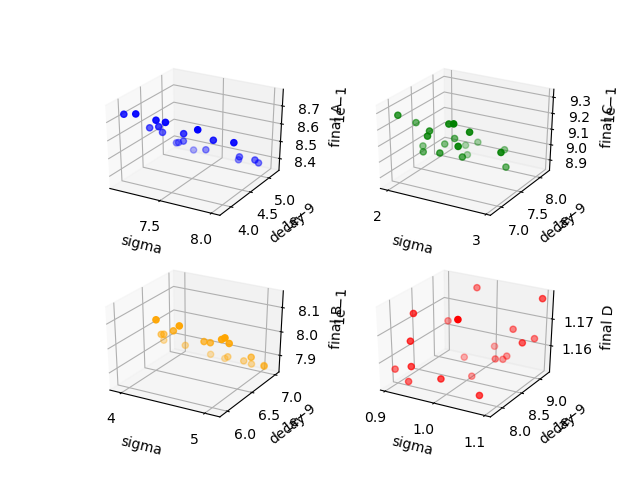
\includegraphics[scale=0.7]{../../tests/framework/user_guide/ForwardSamplingStrategies/gold/RunDir/SparseGrid/1-samplesROMPlot3D_scatter-scatter-scatter-scatter.png}
  \caption{Plot of validation samples generated by Monte Carlo sampling on the ROM for variables $A,B,C,D$.}
  \label{fig:samplesROMSparseGridPlot}
 \end{figure}
 %%%%%%%%%%%%%%%%%%%%%%%%%%%%%%%%%%%%%%%%%%%%%%%%%%%%%%%%%%









\section{Adaptive Sampling Strategies}
\label{sec:adaptiveSamplingStrategies}
Performing UQ and Dynamic PRA can be
challenging from a computational point of view. The \textit{Forward}
sampling strategies reported in the previous Section can lead to a large number of
unnecessary evaluations of the physical model leading to an unacceptable resource expenses (CPU time).
In addition, the \textit{Forward} methodologies are not designed to leverage the information
content that is extractable from the simulations already concluded.

To overcome these limitations, in RAVEN several adaptive algorithms are available:
\begin{enumerate}
  \item \textit{Limit Surface Search}
  \item \textit{Adaptive Dynamic Event Tree}
  \item \textit{Adaptive Hybrid Dynamic Event Tree}
  \item \textit{Adaptive Sparse Grid}
  \item \textit{Adaptive Sobol Decomposition}.
\end{enumerate}
In this Section, we will only show how to use the first algorithm.

%%%%%%%%%%%%%%%%
\subsection{Limit Surface Search sampling through RAVEN}
\label{sub:LSsamplingExample}
The goal of this Section is to learn how to:
 \begin{enumerate}
   \item Set up a LS Search sampling for efficiently perturb a driven code
   \item Use the LS Integral Post-processor for computing the probability of failure of the system subject to the same
   ``goal'' function
   \item Plot the obtained LS.
\end{enumerate}
In order to accomplish these tasks, the following RAVEN \textbf{Entities} (XML blocks in the input files) are defined:
\begin{enumerate}
   \item \textbf{\textit{RunInfo}}:
     \xmlExample[arg,extension,pauseAtEnd,overwrite]{framework/user_guide/AdaptiveSamplingStrategies/adaptiveSamplingLSsearch.xml}{RunInfo}
   As shown in Section~\ref{sub:EntitiesAndFlow}, the \textit{RunInfo} \textbf{Entity} is intended to set up the analysis
   that the user wants to perform. In this specific case, three steps (\xmlNode{Sequence}) are  sequentially run
   using eight processors (\xmlNode{batchSize}).
   \item \textbf{\textit{Files}}:
     \xmlExample[arg,extension,pauseAtEnd,overwrite]{framework/user_guide/AdaptiveSamplingStrategies/adaptiveSamplingLSsearch.xml}{Files}
   Since the driven code uses a single input file, in this Section the original input is placed. As detailed in the user manual
   the attribute  \xmlAttr{name} represents the alias that is going to be
   used in all the other input blocks in order to refer to this file.
   \\In addition the output file used in \xmlNode{Sequence}
   \textit{computeLSintegral} is here inputted.
   \item \textbf{\textit{Models}}:
     \xmlExample[arg,extension,pauseAtEnd,overwrite]{framework/user_guide/AdaptiveSamplingStrategies/adaptiveSamplingLSsearch.xml}{Models}
 As mentioned above, the goal of this example is the employment of
 an efficient sampling strategy, having as goal the determination of the
 failure of a system.

 In addition to the previously explained Code
 model,
 the ROM of type \textit{SciKitLearn} is here specified. The ROM will be
 used in the adaptive sampling strategy \textit{LimitSurfaceSearch} in
 order to accelerate the convergence of the method. As it can be seen,
 a nearest neighbor classifier is used, targeting only two uncertainties
 $sigma-A and decay-A$.
 \\ For the computation of the probability of failure (see the following), a
 Post-Processor (PP) of type \textit{LimitSurfaceIntegral} is here
 specified.This PP performs an integral of the LS
 generated by the adaptive sampling technique.
   \item \textbf{\textit{Distributions}}:
     \xmlExample{framework/user_guide/AdaptiveSamplingStrategies/adaptiveSamplingLSsearch.xml}{Distributions}
  In the Distributions XML Section, the stochastic model for the
  uncertainties  treated by the LS search sampling are reported. In
  this case two distributions are defined:
  \begin{itemize}
    \item $sigmaA \sim \mathbb{U}(0,1000)$, used to model the uncertainty
    associated with  the Model \textit{sigma-A}
    \item  $decayConstantA \sim \mathbb{U}(1e-8,1e-7)$,  used to
    model the uncertainty
    associated with  the Model \textit{decay-A}.
  \end{itemize}
   \item \textbf{\textit{Samplers}}:
     \xmlExample[arg,extension,pauseAtEnd,overwrite]{framework/user_guide/AdaptiveSamplingStrategies/adaptiveSamplingLSsearch.xml}{Samplers}
  In order to employ the LS search sampling strategy, a
  \xmlNode{LimitSurfaceSearch} node needs to be inputted.
  As it can be
  seen from above, each variable is associated to a different distribution
  defined in the  \xmlNode{Distributions} block.
  In addition, the \textit{AccelerationROM}  \xmlNode{ROM} is inputted.
  As already mentioned, this ROM (of type classifier) is used to
  accelerate the convergence of the LS Search method.
  In addition, the goal function \textit{goalFunction}  and the
  \textit{samples} are here reported.
  \\For this example, a convergence criterion of $1.0e-5$ is set. To reach such a confidence with a Monte-Carlo, millions of
  samples would be needed.
   \item \textbf{\textit{Functions}}:
     \xmlExample[arg,extension,pauseAtEnd,overwrite]{framework/user_guide/AdaptiveSamplingStrategies/adaptiveSamplingLSsearch.xml}{Functions}
 As already mentioned, the LS search sampling strategy uses
 a goal function in order to identify the regions of the uncertain space
 that are more informative. The \textit{goalFunction} used for this
 example is reported below. As it can be seen, if the final response $A$
 is $<=$ of $0.3$ , the system is considered to be in a ``safe'' condition.
\begin{lstlisting}[language=python]
def __residuumSign(self):
  returnValue = 1.0
  if self.A  <= 0.3:
    returnValue = -1.0
  return returnValue
\end{lstlisting}

   \item \textbf{\textit{DataObjects}}:
     \xmlExample[arg,extension,pauseAtEnd,overwrite]{framework/user_guide/AdaptiveSamplingStrategies/adaptiveSamplingLSsearch.xml}{DataObjects}
      In this block, three \textit{DataObjects} are defined: 1) PointSet
      named ``samples'' used to collect the final outcomes of the code, 2)
      HistorySet named ``histories'' in which the full time responses of the
      variables $A,B,C,D$ are going to be stored, 3) PointSet named
      ``limitSurface'' used  to export the LS location (in the uncertain space) during the employment of the sampling strategy.
   \item \textbf{\textit{OutStreams}}:
     \xmlExample[arg,extension,pauseAtEnd,overwrite]{framework/user_guide/AdaptiveSamplingStrategies/adaptiveSamplingLSsearch.xml}{OutStreams}
     Several out streams are included in this workflow, two for printing and three for plotting:
     \begin{itemize}
       \item ``samples'', which writes the validation sample contents of the \xmlString{samples} PointSet DataObject to a CSV file,
       \item ``histories'', which writes the sampling contents of the \xmlString{histories} HistorySet DataObject to a
         set of connected CSV files,
       \item ``historyPlot'', which plots the evolution of the samples taken,
       \item ``limitSurfacePlot'', which plots the limit surface discovered by the PostProcessor,
       \item ``samplesPlot3D'', which plots the final state of the samples taken against the figures of merit.
     \end{itemize}
     The plots demonstrate how visualization of three-dimensional data, time-dependent data, and limit
     surfaces can be realized using RAVEN.
 %%%%%%%%%%%%%%%%%%%%%%%%%%%%%%%%%%%%%%%%%%%%%%%%%%%%%%%%%%
 %%%%%%%%%%%%%%%%%%%%%%%%%%%%%%%%%%%%%%%%%%%%%%%%%%%%%%%%%%
 %figure samples
 \begin{figure}[h!]
  \centering
  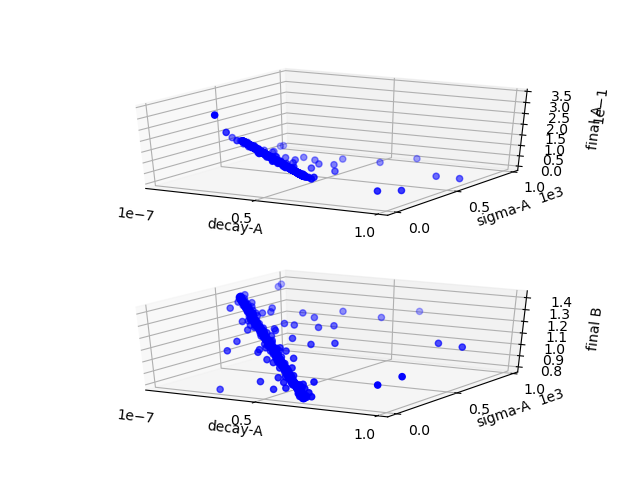
\includegraphics[scale=0.7]{../../tests/framework/user_guide/AdaptiveSamplingStrategies/gold/LSsearch/1-samplesPlot3D_scatter-scatter.png}
  \caption{Plot of the samples generated by the LS search sampling for variables $A,B$.}
  \label{fig:LS_pointsets}
 \end{figure}
 %%%%%%%%%%%%%%%%%%%%%%%%%%%%%%%%%%%%%%%%%%%%%%%%%%%%%%%%%%
 %%%%%%%%%%%%%%%%%%%%%%%%%%%%%%%%%%%%%%%%%%%%%%%%%%%%%%%%%%
   \item \textbf{\textit{Steps}}:
     \xmlExample[arg,extension,pauseAtEnd,overwrite]{framework/user_guide/AdaptiveSamplingStrategies/adaptiveSamplingLSsearch.xml}{Steps}
  %%%%%%%%%%%%%%%%%%%%%%%%%%%%%%%%%%%%%%%%%%%%%%%%%%%%%%%%%%
 %figure samples
 \begin{figure}[h!]
  \centering
  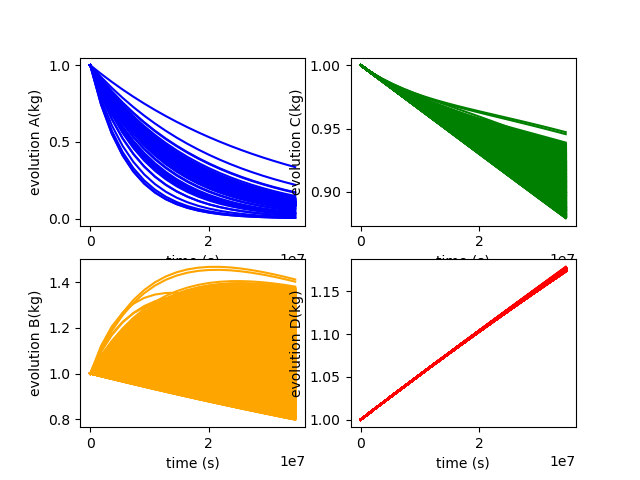
\includegraphics[scale=0.7]{../../tests/framework/user_guide/AdaptiveSamplingStrategies/gold/LSsearch/1-historyPlot_line-line-line-line.png}
  \caption{Plot of the histories generated by the LS search method for variables $A,B,C,D$.}
  \label{fig:LS_histories}
 \end{figure}
 %%%%%%%%%%%%%%%%%%%%%%%%%%%%%%%%%%%%%%%%%%%%%%%%%%%%%%%%%%
   Finally, all the previously defined \textbf{Entities} can be combined in
   the \xmlNode{Steps} block. As inferable,
   three \xmlNode{Steps} have been inputted:
   \begin{itemize}
     \item \xmlNode{MultiRun} named ``sample'', used to run the multiple
     instances of the driven code and
     collect the outputs in the two \textit{DataObjects}. As it can be
     seen, the \xmlNode{Sampler} is inputted to communicate to the
     \textit{Step} that the driven code needs to
     be perturbed through the LS search sampling strategy;
     \item \xmlNode{PostProcess} named ``computeLSintegral'', used to
     compute the probability of failure of the system based on the LS generated employing the LS search strategy. This
     probability is computed integrating the LS with a Monte-Carlo
     method.
     \item  \xmlNode{IOStep} named ``writeHistories'', used to 1) export
     the ``histories'' and ``samples''  \textit{DataObjects}
     \textbf{Entity} in a CSV file and 2) plot the data and the Limit Surface
     in  PNG files and on the screen.
   \end{itemize}
\end{enumerate}
 Figure~\ref{fig:LS_histories}
 shows the evolution of the outputs $A,B,C,D$ under uncertainties.
 Figure~\ref{fig:LS_pointsets} shows the final responses  of $A and B$
 of the sampling employed using the driven code.
 Figure~\ref{fig:LSplot}  shows the limit surface for this particular
 example. Only $367$ samples were needed in order to reach the full
 convergence.
 \\The integration of the LS determines a probability of failure of
 $~3.45e-2$.
  %%%%%%%%%%%%%%%%%%%%%%%%%%%%%%%%%%%%%%%%%%%%%%%%%%%%%%%%%%
 %figure samples
 \begin{figure}[h!]
  \centering
  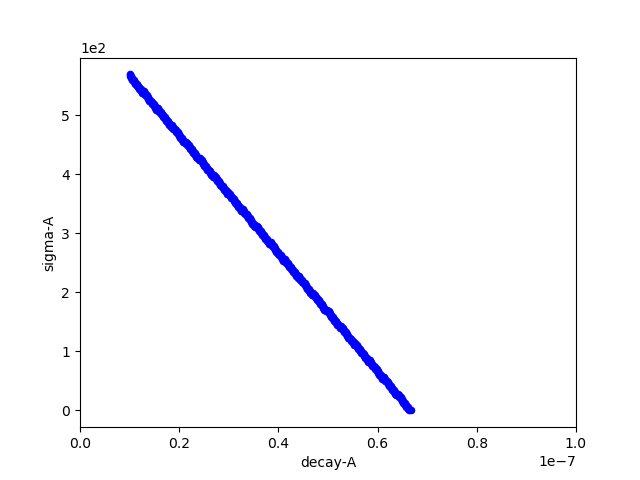
\includegraphics[scale=0.7]{../../tests/framework/user_guide/AdaptiveSamplingStrategies/gold/LSsearch/1-limitSurfacePlot_scatter.png}
  \caption{Limit Surface generated by the LS search method.}
  \label{fig:LSplot}
 \end{figure}
 %%%%%%%%%%%%%%%%%%%%%%%%%%%%%%%%%%%%%%%%%%%%%%%%%%%%%%%%%%









\section{Sampling from Restart}
\label{sec:samplingFromRestart}
In some instances, there are existing solutions stored that are useful to a new sampling calculation.  For
example, if a Monte Carlo run collects 1000 runs, then later the user decides to expand to 1500 runs, the
original 1000 should not be wasted.  In this case, it is desirable to restart sampling.

All \xmlNode{Sampler} entities in RAVEN accept the \xmlNode{Restart} node, which allows the user to provide a
\xmlNode{DataObject} from which sampling can draw.  The way each sampler interacts with this restart data is
dependent on the sampling strategy.

Random sampling strategies, such as the \xmlNode{MonteCarlo} and \xmlNode{Stratified} samplers, increment the
random number generator by the number of samples in the restart data, then continue sampling as normal.

Grid-based sampling strategies, such as \xmlNode{Grid}, \xmlNode{SparseGridCollocation}, and \xmlNode{Sobol},
require specific sampling points.  As each required point in the input space is determined, the sampler will
check the restart data for a match.  If a match is found, the corresponding output values are used instead of
sampling the \xmlNode{Model} for that point in the input space.  In order to determine a match, all of the
values in the restart point must be within a relative tolerance of the corresponding point required by the
sampler.  While RAVEN has a default tolerance of 1e-15, the user can adjust this tolerance using the
\xmlNode{restartNode} node in the \xmlNode{Sampler} block.

In order to demonstrate this restart method, we include here an example of restarting a \xmlNode{Grid}
sampler.  This example runs a simple example Python code from the command line using the \xmlNode{GenericCode}
interface.  Within the run the following steps occur:
\begin{enumerate}
  \item A grid is sampled that includes only the endpoints in each dimension.
  \item The results of the first sampling are written to file.
  \item The results in the CSV are read back in to a new \xmlNode{DataObject} called \xmlString{restart}.
  \item A second, more dense grid is sampled that requires the points of the first sampling, plus several
    more.  The results are added both to the original \xmlNode{DataObject} as well as a new one, for
    demonstration purposes.
  \item The results of only the new sampling can be written to CSV because we added the second data object in
    the last step.
  \item Lastly, the complete \xmlNode{DataObject} is written to file, including both the original and more
    dense sampling.
\end{enumerate}
By looking at the contents of \texttt{GRIDdump1.csv}, \texttt{GRIDdump2.csv}, and \texttt{GRIDdump3.csv}, the
progressive construction of the data object becomes clear.  \texttt{GRIDdump1.csv} contains only a few samples
corresponding to the endpoints of the distributions.  \texttt{GRIDdump3.csv} contains all the points necessary
to include the midpoints of the distributions as well as the endpoints.  \texttt{GRIDdump2.csv} contains only
those points that were not already obtained in the first sampling, but still needed for the more dense
sampling.

\xmlExample[coarse,fine,restart]{framework/Samplers/Restart/Truncated/grid.xml}{Simulation}

In order to restart an existing file that failed for some reason, the
data will need to be listed in the \xmlNode{Files} section and a
\xmlNode{IOStep} that loads that input into a different data object
will be needed to be added to the \xmlNode{Steps} section. After that a \xmlNode{Restart} node can be added.

\xmlExample{framework/Samplers/Restart/test_restart_Grid_part2.xml}{Files}

\xmlExample{framework/Samplers/Restart/test_restart_Grid_part2.xml}{Steps}

\xmlExample{framework/Samplers/Restart/test_restart_Grid_part2.xml}{Samplers}

\section{Reduced Order Modeling through RAVEN}
\label{sec:ROMraven}
The development of high-fidelity codes, for thermal-hydraulic systems
and integrated multi-physics, has undergone a significant acceleration
in the last years. Multi-physics codes simulate
multiple physical models or multiple simultaneous physical phenomena,
in a integrated solving environment. Multi-physics typically
solves coupled systems of partial differential equations, generally
characterized by several different geometrical and time scales.

The new multi-physics codes are characterized by remarkable
improvements
in the approximation of physics (high approximation order and reduced
use of empirical correlations). This greater fidelity is generally
accompanied by a greater computational effort (calculation time
increased). This peculiarity is an
obstacle in the application of  computational techniques of
quantification of uncertainty and risk associated with the operation of
particular industrial plant (e.g., a nuclear reactor).

A solution to this problem is represented by the
usage
of highly effective sampling strategies. Sometimes also these
approaches is not enough
in order to perform a comprehensive UQ and PRA analysis. In these
cases the help of reduced order modeling is essential.

RAVEN has support of several different ROMs,
such as:
\begin{enumerate}
  \item \textit{Nearest Neighbors approaches}
  \item \textit{Support Vector Machines}
  \item \textit{Inverse Weight regressors}
  \item \textit{Spline regressors }, etc.
\end{enumerate}

A ROM, also known a surrogate
model, is a mathematical representation of a system, used to predict
a FOM of a physical system.

The ``training'' is a process of setting the internal parameters of the ROM from a set
of samples generated the physical model, .e.,
 the high-fidelity simulator (RELAP-7, RELAP5
3D, PHISICS, etc.),
\begin{figure}[h!]
  \centering
  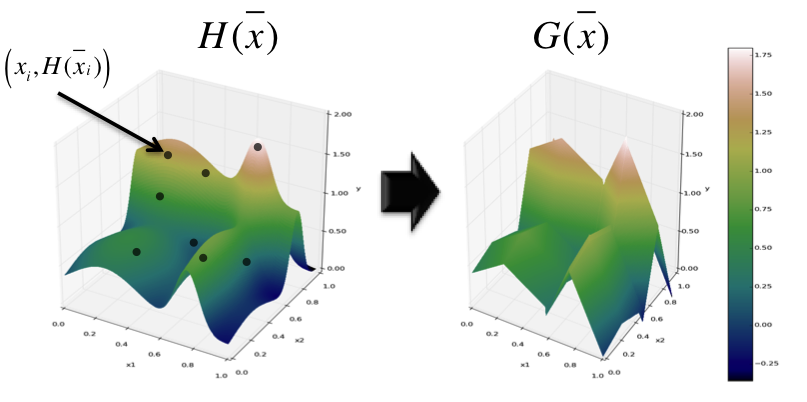
\includegraphics[width=1.0\textwidth]  {pics/ROMexampleOfPhysicalSystem.png}
  \caption{Example of reduced order model representation of physical system (regression).}
  \label{fig:ROMexampleOfPhysicalSystem}
\end{figure}

Two characteristics of these models
are generally assumed (even if exceptions are possible):
\begin{enumerate}
  \item The higher the number of realizations in the training sets, the
higher is the accuracy of the prediction performed by the ROM is. This
statement is true for most of the cases, although some ROMs might be
subject to the over-fitting issues. The over-fitting phenomenon is not
analyzed in this thesis, since its occurrence highly depends on the
algorithm type, and, hence, the problem needs to be analyzed for all
the large number of ROM types available;
  \item The smaller the size of the input (uncertain) domain with
  respect to the variability of the system response, the more likely the
  ROM is able to represent the system response space.
\end{enumerate}

The goals of this section are about learning how to:
 \begin{enumerate}
   \item Set up a sampling strategy to construct multiple ROMs, perturbing a driven code
   \item Train the different ROMs with the data-set obtained by the applied sampling strategy;
   \item Use the same sampling strategy, perturbing the ROMs
   \item Plot the responses of the driven code and ROMs, respectively.
\end{enumerate}
In order to accomplish these tasks, the following RAVEN \textbf{Entities} (XML blocks in the input files) need to be defined:
\begin{enumerate}
   \item \textbf{\textit{RunInfo}}:
     \xmlExample{framework/user_guide/ReducedOrderModeling/reducedOrderModeling.xml}{RunInfo}
   As in the other examples, the the \textit{RunInfo} \textbf{Entity} is intended  to set up the analysis sequence that
   needs to be performed. In this specific case, eight steps  (\xmlNode{Sequence}) are going to be sequentially run
   using eight processors (\xmlNode{batchSize}).
   \\In the first step, the original physical model is going to be sampled. The obtained results are going to be used to
   train three different ROMs.These ROMs are sampled by the same strategy used in the first step in order to compare the
   ROMs' responses with the ones coming from the original physical model.
   \item \textbf{\textit{Files}}:
     \xmlExample{framework/user_guide/ReducedOrderModeling/reducedOrderModeling.xml}{Files}
   Since the driven code uses a single input file, the original input is placed in this section. As detailed in the user manual
   the attribute  \xmlAttr{name} represents the alias that is going to be
   used in all the other input blocks in order to refer to this file.
   \item \textbf{\textit{Models}}:
     \xmlExample{framework/user_guide/ReducedOrderModeling/reducedOrderModeling.xml}{Models}
 As mentioned above, the goal of this example is the employment of
 a sampling strategy in order to construct multiple types of ROMs.
 \\Indeed, in addition to the previously explained Code
 model,
 three different ROMs (GP, SVM and IDW) are here specified. The ROMs will be
 constructed (``trained'') through the data-set generated by the sampling of the physical model. Once trained, they are going
 to be used in place of the original physical model.
 \\As it can be seen,
 the ROMs will be constructed considering four features ($sigma-A,\,sigma-B,\, decay-A \,,and \, decay-B$) and two targets
 ($A \, and \, B$).
   \item \textbf{\textit{Distributions}}:
     \xmlExample{framework/user_guide/ReducedOrderModeling/reducedOrderModeling.xml}{Distributions}
  In the Distributions XML section, the stochastic model for the
  uncertainties are reported. In
  this case two distributions are defined:
  \begin{itemize}
    \item $sigma \sim \mathbb{U}(0,1000)$, used to model the uncertainties
    associated with  the Model \textit{sigma-A} and \textit{sigma-B};
    \item  $decayConstant \sim \mathbb{U}(1e-8,1e-7)$,  used to
    model the uncertainties
    associated with  the Model \textit{decay-A} and \textit{decay-B}.
  \end{itemize}
   \item \textbf{\textit{Samplers}}:
     \xmlExample{framework/user_guide/ReducedOrderModeling/reducedOrderModeling.xml}{Samplers}
  To obtain the data-set through which the ROMs are going to be
  constructed, a \textit{Grid} sampling approach is here employed.
   \item \textbf{\textit{DataObjects}}:
     \xmlExample{framework/user_guide/ReducedOrderModeling/reducedOrderModeling.xml}{DataObjects}
  Int this block, six \textit{DataObjects} are defined: 1) PointSet
  named ``samples'' used to collect the final outcomes of the code, 2)
  HistorySet named ``histories'' in which the full time responses of the
  variables $A,B,C,D$ are going to be stored, 3) PointSet named
  ``inputPlaceHolder'' used in the \textit{role} of \xmlNode{Input} for the ROMs sampling;
  4) PointSet named ``samplesGP'' used to collect the final outcomes (sampling) of the GP ROM;
  5) PointSet named ``samplesInverse'' used to collect the final outcomes (sampling) of the IDW ROM;
  6) PointSet named ``samplesSVM'' used to collect the final outcomes (sampling) of the SVM ROM.
 %%%%%%%%%%%%%%%%%%%%%%%%%%%%%%%%%%%%%%%%%%%%%%%%%%%%%%%%%%
 %%%%%%%%%%%%%%%%%%%%%%%%%%%%%%%%%%%%%%%%%%%%%%%%%%%%%%%%%%
 %figure samples
 \begin{figure}[h!]
  \centering
  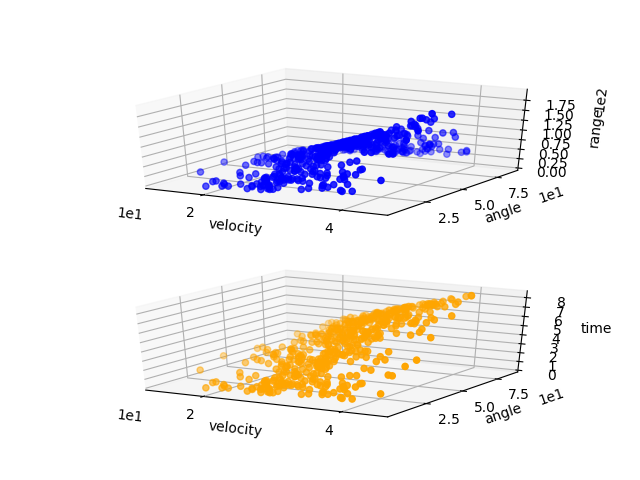
\includegraphics[scale=0.7]{../../tests/framework/user_guide/ReducedOrderModeling/gold/ROMConstruction/1-samplesPlot3D_scatter-scatter.png}
  \caption{Plot of the samples generated by the Grid sampling for variables $A,B$.}
  \label{fig:ROMgrid_pointsets}
 \end{figure}
 %%%%%%%%%%%%%%%%%%%%%%%%%%%%%%%%%%%%%%%%%%%%%%%%%%%%%%%%%%
 %%%%%%%%%%%%%%%%%%%%%%%%%%%%%%%%%%%%%%%%%%%%%%%%%%%%%%%%%%
   \item \textbf{\textit{OutStreams}}:
     \xmlExample{framework/user_guide/ReducedOrderModeling/reducedOrderModeling.xml}{OutStreams}
     This model makes use of two Print OutStreams and five Plot OutStreams:
     \begin{itemize}
       \item ``samples,'' which writes the contents of the point-wise training samples to CSV,
       \item ``histories,'' which writes the contents of the history-wise training samples to linked CSVs,
       \item ``historyPlot,'' which plots the evolution of the training samples,
       \item ``samplesPlot3D,'' which plots the final state of the training samples with relation to the
         outputs of interest,
       \item ``samplesPlot3DROMgp,'' which plots the validation samples of the Gaussian Process ROM,
       \item ``samplesPlot3DROMsvm,'' which plots the validation samples of the Support-Vector Machine ROM,
       \item ``samplesPlot3Dinverse,'' which plots the validation samples of the multidimensional Inverse
         Weight ROM.
     \end{itemize}
     The 3D plots of the samples as well as the ROM samples can be used as a view-norm validation of the ROMs.
   \item \textbf{\textit{Steps}}:
     \xmlExample{framework/user_guide/ReducedOrderModeling/reducedOrderModeling.xml}{Steps}
  %%%%%%%%%%%%%%%%%%%%%%%%%%%%%%%%%%%%%%%%%%%%%%%%%%%%%%%%%%
 %figure samples
 \begin{figure}[h!]
  \centering
  \includegraphics[scale=0.7]{../../tests/framework/user_guide/ReducedOrderModeling/gold/ROMConstruction/1-historyPlot_line-line-line-line.png}
  \caption{Plot of the histories generated by the Grid method for variables $A,B,C,D$.}
  \label{fig:ROMgrid_histories}
 \end{figure}
   %%%%%%%%%%%%%%%%%%%%%%%%%%%%%%%%%%%%%%%%%%%%%%%%%%%%%%%%%%
 %figure samples
 \begin{figure}[h!]
  \centering
  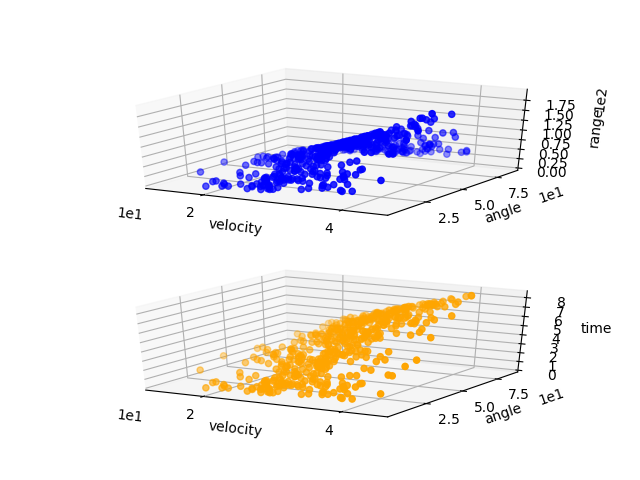
\includegraphics[scale=0.7]{../../tests/framework/user_guide/ReducedOrderModeling/gold/ROMConstruction/1-samplesPlot3DROMgp_scatter-scatter.png}
  \caption{Plot of the samples generated by the Grid sampling applied on the Gaussian Process ROM for variables $A,B$}
  \label{fig:ROMgp_samples}
 \end{figure}
 %%%%%%%%%%%%%%%%%%%%%%%%%%%%%%%%%%%%%%%%%%%%%%%%%%%%%%%%%%
 %%%%%%%%%%%%%%%%%%%%%%%%%%%%%%%%%%%%%%%%%%%%%%%%%%%%%%%%%%
   Finally, all the previously defined \textbf{Entities} can be combined in
   the \xmlNode{Steps} block. As inferable,
   eight \xmlNode{Steps} have been inputted:
   \begin{itemize}
     \item \xmlNode{MultiRun} named ``sample'', used to run the multiple
     instances of the driven code and
     collect the outputs in the two \textit{DataObjects}. As it can be
     seen, the \xmlNode{Sampler} is inputted to communicate to the
     \textit{Step} that the driven code needs to
     be perturbed through the Grid sampling strategy;
     \item \xmlNode{RomTrainer} named ``trainROMGaussianProcess'', used to construct (``train'')
     the GP ROM, based on the data-set generated in the  ``sample'' \textbf{Step};
     \item \xmlNode{RomTrainer} named ``trainROMsvm'', used to construct (``train'')
     the SVM ROM, based on the data-set generated in the  ``sample'' \textbf{Step};
     \item \xmlNode{RomTrainer} named ``trainROMinverse'', used to construct (``train'')
     the IDW ROM, based on the data-set generated in the  ``sample'' \textbf{Step};
     \item \xmlNode{MultiRun} named ``sampleROMGaussianProcess'', used to run the multiple
     instances of the previously constructed GP ROM and
     collect the outputs in the PointSet \textit{DataObject}. As it can be
     seen, the same \xmlNode{Sampler} used for perturbing the original model is here used.
     \item \xmlNode{MultiRun} named ``sampleROMsvm'', used to run the multiple
     instances of the previously constructed Support Vector Machine ROM and
     collect the outputs in the PointSet \textit{DataObject}. As it can be
     seen, the same \xmlNode{Sampler} used for perturbing the original model is here used.
     \item \xmlNode{MultiRun} named ``sampleROMInverse'', used to run the multiple
     instances of the previously constructed Inverse Distance Weight ROM and
     collect the outputs in the PointSet \textit{DataObject}. As it can be
     seen, the same \xmlNode{Sampler} used for perturbing the original model is here used.
     \item  \xmlNode{IOStep} named ``writeHistories'', used to 1) export
     the ``histories'' and ``samples''  \textit{DataObjects}
     \textbf{Entity} in a CSV file and 2) plot the responses of the sampling performed on the physical model, GP ROM,
     SVM ROM and IDW ROM in  PNG files and on the screen.
   \end{itemize}
\end{enumerate}

  %figure samples
 \begin{figure}[h!]
  \centering
  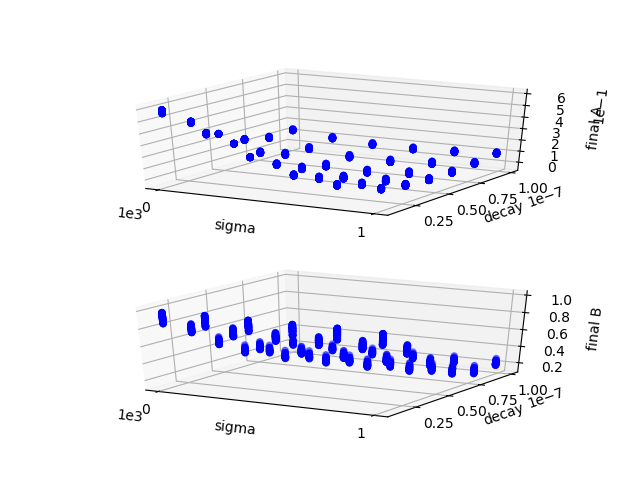
\includegraphics[scale=0.7]{../../tests/framework/user_guide/ReducedOrderModeling/gold/ROMConstruction/1-samplesPlot3DROMsvm_scatter-scatter.png}
  \caption{Plot of the samples generated by the Grid sampling applied on the Support Vector Machine ROM for variables $A,B$}
  \label{fig:ROMsvm_samples}
 \end{figure}
 %%%%%%%%%%%%%%%%%%%%%%%%%%%%%%%%%%%%%%%%%%%%%%%%%%%%%%%%%%
  %%%%%%%%%%%%%%%%%%%%%%%%%%%%%%%%%%%%%%%%%%%%%%%%%%%%%%%%%%
  %figure samples
 \begin{figure}[h!]
  \centering
  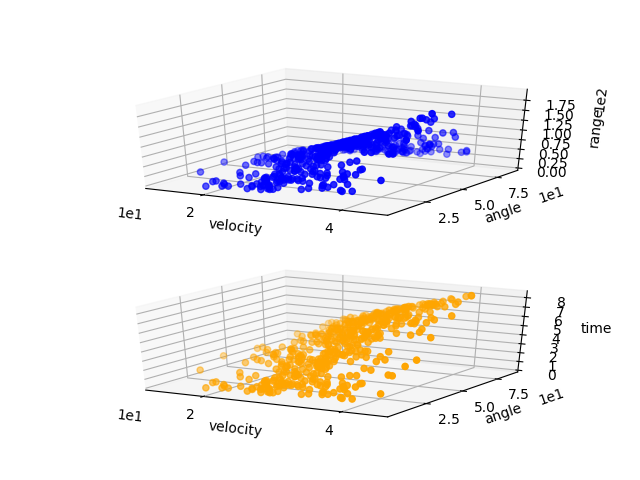
\includegraphics[scale=0.7]{../../tests/framework/user_guide/ReducedOrderModeling/gold/ROMConstruction/1-samplesPlot3DROMinverse_scatter-scatter.png}
  \caption{Plot of the samples generated by the Grid sampling applied on the Inverse Distance Weight ROM for variables $A,B$}
  \label{fig:ROMinverse_samples}
 \end{figure}
 %%%%%%%%%%%%%%%%%%%%%%%%%%%%%%%%%%%%%%%%%%%%%%%%%%%%%%%%%%
 Figure \ref{fig:ROMgrid_histories}
 shows the evolution of the outputs $A,B,C,D$ under uncertainties.
 Figure \ref{fig:ROMgrid_pointsets} shows the final responses  of $A and B$
 of the sampling employed using the driven code.

Figures \ref{fig:ROMgp_samples}, \ref{fig:ROMsvm_samples} and \ref{fig:ROMinverse_samples}  show the final responses  of $A and B$ of the sampling employed using the Gaussian Process, Support Vector Machines and Inverse Distance Weight ROMs, respectively.
It can be clearly noticed that the responses of the ROMs perfectly match the outcomes coming from the original model (see Figure   \ref{fig:ROMgrid_pointsets}).









\section{Statistical Analysis through RAVEN}
\label{sec:SAraven}
In order to perform a complete analysis of a system under uncertainties,
it is crucial to be able to compute all the statistical moments of one or even multiple
FOMs. In addition, it is essential to identify the correlation
among different FOMs toward a specific input space.

RAVEN is able to compute the most important statistical moments:
such as:
\begin{enumerate}
  \item \textit{Expected Value}
  \item \textit{Standard Deviation}
  \item \textit{Variance}
  \item \textit{variationCoefficient}
  \item \textit{Skewness}
  \item \textit{Kurtosis}
  \item \textit{Median}
  \item \textit{Percentile}.
\end{enumerate}
In addition, RAVEN fully supports the computation of all of the statistical moments defined to
``measure'' the correlation among variables/parameters/FOMs:
\begin{enumerate}
  \item \textit{Covariance matrix}
  \item \textit{Normalized Sensitivity  matrix}
  \item \textit{Variance Dependent Sensitivity  matrix}
  \item \textit{Sensitivity matrix}
  \item \textit{Pearson matrix}.
\end{enumerate}
The goals of this section is to show how to:
 \begin{enumerate}
   \item Set up a sampling strategy to perform a final statistical analysis
   perturbing a driven code
   \item Compute all the statistical moments and correlation/covariance
   metrics.
\end{enumerate}
In order to accomplish these tasks, the following RAVEN \textbf{Entities} (XML blocks in the input files) need to be defined:
\begin{enumerate}
   \item \textbf{\textit{RunInfo}}:
     \xmlExample{framework/user_guide/StatisticalAnalysis/statisticalAnalysis.xml}{RunInfo}
   As shown in the other examples, the \textit{RunInfo} \textbf{Entity} is intended  to set up the desired analysis . In this specific case, two steps  (\xmlNode{Sequence}) are  sequentially run
   using forty processors (\xmlNode{batchSize}).
   \\In the first step, the original physical model is sampled. The obtained results are  analyzed with the Statistical Post-Processor.
   \item \textbf{\textit{Files}}:
     \xmlExample{framework/user_guide/StatisticalAnalysis/statisticalAnalysis.xml}{Files}
   Since the driven code uses a single input file, in this section the original input is placed. As detailed in the user manual
   the attribute  \xmlAttr{name} represents the alias that is going to be
   used in all the other input blocks in order to refer to this file.
   \\In addition, the output file of the \textit{PostProcess} \textbf{Step} is
   here defined (XML format).
   \item \textbf{\textit{Models}}:
     \xmlExample{framework/user_guide/StatisticalAnalysis/statisticalAnalysis.xml}{Models}
 The goal of this example is to show how the
 principal statistical FOMs can be computed through RAVEN.
 \\Indeed, in addition to the previously explained Code
 model, a Post-Processor model (BasicStatistics) is here specified.
Note that the post-process step is
performed on all the variables with respect to the parameters used in this example ( $A,\, B,\, C \, and \, D$
with respect to $sigma-A,\,sigma-B,\, decay-A,$ and $decay-B$).
   \item \textbf{\textit{Distributions}}:
     \xmlExample{framework/user_guide/StatisticalAnalysis/statisticalAnalysis.xml}{Distributions}
  In the Distributions XML section, the stochastic models for the
  uncertainties are reported. In
  this case 2 distributions are defined:
  \begin{itemize}
    \item $sigma \sim \mathbb{U}(0,1000)$, used to model the uncertainties
    associated with  the Model \textit{sigma-A} and \textit{sigma-B}
    \item  $decayConstant \sim \mathbb{U}(1e-8,1e-7)$,  used to
    model the uncertainties
    associated with  the Model \textit{decay-A} and \textit{decay-B}.
  \end{itemize}
   \item \textbf{\textit{Samplers}}:
     \xmlExample{framework/user_guide/StatisticalAnalysis/statisticalAnalysis.xml}{Samplers}
  In order to obtained the data-set through which the statistical FOMs need to be computed, a \textit{MonteCarlo} sampling approach is here employed.
   \item \textbf{\textit{DataObjects}}:
     \xmlExample{framework/user_guide/StatisticalAnalysis/statisticalAnalysis.xml}{DataObjects}
  Int this block, two \textit{DataObjects} are defined:
  1) PointSet named ``samplesMC'' used to collect the final outcomes of
  the code,
  2) HistorySet named ``histories'' in which the full time responses of the
  variables $A,B,C,D$ are going to be stored.

   \item \textbf{\textit{Steps}}:
     \xmlExample{framework/user_guide/StatisticalAnalysis/statisticalAnalysis.xml}{Steps}

 %%%%%%%%%%%%%%%%%%%%%%%%%%%%%%%%%%%%%%%%%%%%%%%%%%%%%%%%%%
 %%%%%%%%%%%%%%%%%%%%%%%%%%%%%%%%%%%%%%%%%%%%%%%%%%%%%%%%%%
   Finally, all the previously defined \textbf{Entities} can be combined in
   the \xmlNode{Steps} block. As inferable,
   2 \xmlNode{Steps} have been inputted:
   \begin{itemize}
     \item \xmlNode{MultiRun} named ``sampleMC'', used to run the
     multiple
     instances of the driven code and
     collect the outputs in the two \textit{DataObjects}. As it can be
     seen, the \xmlNode{Sampler} is inputted to communicate to the
     \textit{Step} that the driven code needs to
     be perturbed through the Grid sampling strategy.
     \item \xmlNode{PostProcess} named ``statisticalAnalysisMC'', used
     compute all the statistical moments and FOMs based on the
     data obtained through the sampling strategy. As it can be noticed,
     the \xmlNode{Output} of the ``sampleMC'' \textit{Step} is the
     \xmlNode{Input} of the ``statisticalAnalysisMC''  \textit{Step}.
   \end{itemize}
\end{enumerate}

Tables \ref{ScalarMoments}-\ref{SensitivityComputed} show all the results of the \textit{PostProcess}
step.


\begin{landscape}
\begin{table}[h!]
\centering
\caption{Computed Moments and Cumulants.}
\label{ScalarMoments}
\begin{tabular}{|c|c|c|c|c|c|c|c|c|}
\hline
{\ul \textit{\textbf{Computed Quantities}}} & \textbf{A} & \textbf{B} & \textbf{C} & \textbf{D} & \textbf{decay-A} & \textbf{decay-B} & \textbf{sigma-A} & \textbf{sigma-B} \\ \hline
\textit{expected value}                     & 5.97E-02   & 3.97E-01   & 9.82E-01   & 1.50E+00   & 5.57E-08         & 5.61E-08         & 5.07E+02         & 4.73E+02         \\ \hline
\textit{median}                             & 2.45E-02   & 3.06E-01   & 9.89E-01   & 1.54E+00   & 5.73E-08         & 5.62E-08         & 5.11E+02         & 4.70E+02         \\ \hline
\textit{variance}                           & 8.19E-03   & 6.00E-02   & 1.19E-02   & 1.49E-02   & 7.00E-16         & 6.83E-16         & 8.52E+04         & 8.64E+04         \\ \hline
\textit{sigma}                              & 9.05E-02   & 2.45E-01   & 1.09E-01   & 1.22E-01   & 2.64E-08         & 2.61E-08         & 2.92E+02         & 2.94E+02         \\ \hline
\textit{variation coefficient}              & 1.52E+00   & 6.17E-01   & 1.11E-01   & 8.15E-02   & 4.75E-01         & 4.66E-01         & 5.75E-01         & 6.21E-01         \\ \hline
\textit{skewness}                           & 2.91E+00   & 9.88E-01   & -1.49E-01  & -9.64E-01  & -6.25E-02        & -5.75E-02        & -2.18E-02        & 7.62E-02         \\ \hline
\textit{kurtosis}                           & 9.56E+00   & -1.12E-01  & -6.98E-01  & -1.50E-01  & -1.24E+00        & -1.21E+00        & -1.21E+00        & -1.20E+00        \\ \hline
\textit{percentile 5\%}                     & 2.87E-03   & 1.48E-01   & 7.89E-01   & 1.24E+00   & 1.42E-08         & 1.45E-08         & 5.08E+01         & 2.97E+01         \\ \hline
\textit{percentile 95\%}                    & 2.51E-01   & 9.19E-01   & 1.16E+00   & 1.63E+00   & 9.54E-08         & 9.48E-08         & 9.59E+02         & 9.49E+02         \\ \hline
\end{tabular}
\end{table}
\begin{table}[h!]
\centering
\caption{Covariance matrix.}
\label{covarianceComputed}
\begin{tabular}{|c|c|c|c|c|c|c|c|c|}
\hline
{\ul \textit{\textbf{Covariance}}} & \textbf{A} & \textbf{B} & \textbf{C} & \textbf{D} & \textbf{decay-A} & \textbf{decay-B} & \textbf{sigma-A} & \textbf{sigma-B} \\ \hline
\textbf{A}                         & 8.19E-03   & -1.11E-03  & -3.09E-03  & -1.13E-04  & -1.28E-09        & 5.14E-11         & -1.49E+01        & -3.74E-01        \\ \hline
\textbf{B}                         & -1.11E-03  & 6.00E-02   & 2.26E-03   & -2.96E-02  & -7.80E-11        & -6.02E-09        & 7.00E+00         & -1.47E+00        \\ \hline
\textbf{C}                         & -3.09E-03  & 2.26E-03   & 1.19E-02   & 7.15E-04   & -1.44E-09        & -4.11E-12        & 2.63E+01         & 3.19E-01         \\ \hline
\textbf{D}                         & -1.13E-04  & -2.96E-02  & 7.15E-04   & 1.49E-02   & -1.21E-10        & 3.01E-09         & 1.12E+00         & 8.01E-01         \\ \hline
\textbf{decay-A}                   & -1.28E-09  & -7.80E-11  & -1.44E-09  & -1.21E-10  & 7.00E-16         & -1.73E-17        & -1.26E-07        & 2.07E-07         \\ \hline
\textbf{decay-B}                   & 5.14E-11   & -6.02E-09  & -4.11E-12  & 3.01E-09   & -1.73E-17        & 6.83E-16         & -1.86E-07        & 3.91E-08         \\ \hline
\textbf{sigma-A}                   & -1.49E+01  & 7.00E+00   & 2.63E+01   & 1.12E+00   & -1.26E-07        & -1.86E-07        & 8.52E+04         & 1.79E+03         \\ \hline
\textbf{sigma-B}                   & -3.74E-01  & -1.47E+00  & 3.19E-01   & 8.01E-01   & 2.07E-07         & 3.91E-08         & 1.79E+03         & 8.64E+04         \\ \hline
\end{tabular}
\end{table}
\begin{table}[h!]
\centering
\caption{Correlation matrix.}
\label{pearsonComputed}
\begin{tabular}{|c|c|c|c|c|c|c|c|c|}
\hline
{\ul \textit{\textbf{Correlation}}} & \textbf{A} & \textbf{B} & \textbf{C} & \textbf{D} & \textbf{decay-A} & \textbf{decay-B} & \textbf{sigma-A} & \textbf{sigma-B} \\ \hline
\textbf{A}                          & 1.00E+00   & -5.02E-02  & -3.13E-01  & -1.03E-02  & -5.35E-01        & 2.17E-02         & -5.63E-01        & -1.40E-02        \\ \hline
\textbf{B}                          & -5.02E-02  & 1.00E+00   & 8.47E-02   & -9.90E-01  & -1.20E-02        & -9.41E-01        & 9.80E-02         & -2.04E-02        \\ \hline
\textbf{C}                          & -3.13E-01  & 8.47E-02   & 1.00E+00   & 5.37E-02   & -4.98E-01        & -1.44E-03        & 8.25E-01         & 9.96E-03         \\ \hline
\textbf{D}                          & -1.03E-02  & -9.90E-01  & 5.37E-02   & 1.00E+00   & -3.75E-02        & 9.43E-01         & 3.14E-02         & 2.23E-02         \\ \hline
\textbf{decay-A}                    & -5.35E-01  & -1.20E-02  & -4.98E-01  & -3.75E-02  & 1.00E+00         & -2.50E-02        & -1.64E-02        & 2.67E-02         \\ \hline
\textbf{decay-B}                    & 2.17E-02   & -9.41E-01  & -1.44E-03  & 9.43E-01   & -2.50E-02        & 1.00E+00         & -2.44E-02        & 5.08E-03         \\ \hline
\textbf{sigma-A}                    & -5.63E-01  & 9.80E-02   & 8.25E-01   & 3.14E-02   & -1.64E-02        & -2.44E-02        & 1.00E+00         & 2.08E-02         \\ \hline
\textbf{sigma-B}                    & -1.40E-02  & -2.04E-02  & 9.96E-03   & 2.23E-02   & 2.67E-02         & 5.08E-03         & 2.08E-02         & 1.00E+00         \\ \hline
\end{tabular}
\end{table}
\begin{table}[h!]
\centering
\caption{Variance Dependent Sensitivity matrix.}
\label{VarDepSensitivityComputed}
\begin{tabular}{|c|c|c|c|c|c|c|c|c|}
\hline
{\ul \textit{\textbf{Variance Sensitivity}}} & \textbf{A} & \textbf{B} & \textbf{C} & \textbf{D} & \textbf{decay-A} & \textbf{decay-B} & \textbf{sigma-A} & \textbf{sigma-B} \\ \hline
\textbf{A}                                   & 1.00E+00   & -1.36E-01  & -3.77E-01  & -1.38E-02  & -1.56E-07        & 6.27E-09         & -1.82E+03        & -4.56E+01        \\ \hline
\textbf{B}                                   & -1.86E-02  & 1.00E+00   & 3.77E-02   & -4.94E-01  & -1.30E-09        & -1.00E-07        & 1.17E+02         & -2.45E+01        \\ \hline
\textbf{C}                                   & -2.60E-01  & 1.90E-01   & 1.00E+00   & 6.01E-02   & -1.21E-07        & -3.46E-10        & 2.21E+03         & 2.68E+01         \\ \hline
\textbf{D}                                   & -7.60E-03  & -1.99E+00  & 4.80E-02   & 1.00E+00   & -8.11E-09        & 2.02E-07         & 7.51E+01         & 5.37E+01         \\ \hline
\textbf{decay-A}                             & -1.83E+06  & -1.11E+05  & -2.05E+06  & -1.73E+05  & 1.00E+00         & -2.47E-02        & -1.81E+08        & 2.96E+08         \\ \hline
\textbf{decay-B}                             & 7.52E+04   & -8.82E+06  & -6.02E+03  & 4.40E+06   & -2.53E-02        & 1.00E+00         & -2.72E+08        & 5.72E+07         \\ \hline
\textbf{sigma-A}                             & -1.75E-04  & 8.22E-05   & 3.08E-04   & 1.32E-05   & -1.48E-12        & -2.19E-12        & 1.00E+00         & 2.10E-02         \\ \hline
\textbf{sigma-B}                             & -4.33E-06  & -1.70E-05  & 3.69E-06   & 9.27E-06   & 2.40E-12         & 4.52E-13         & 2.07E-02         & 1.00E+00         \\ \hline
\end{tabular}
\end{table}
\begin{table}[h!]
\centering
\caption{Sensitivity matrix.}
\label{SensitivityComputed}
\begin{tabular}{|c|c|c|c|c|}
\hline
{\ul \textit{\textbf{Sensitivity (I/O)}}} & \textbf{decay-A} & \textbf{decay-B} & \textbf{sigma-A} & \textbf{sigma-B} \\ \hline
\textbf{A}                                & 3.83E-06         & -1.78E-04        & -2.07E+04        & -1.86E+06        \\ \hline
\textbf{B}                                & -1.36E-05        & 6.28E-05         & -8.80E+06        & -3.14E+05        \\ \hline
\textbf{C}                                & 2.17E-06         & 3.05E-04         & 2.64E+04         & -2.00E+06        \\ \hline
\textbf{D}                                & 6.96E-06         & 2.25E-05         & 4.40E+06         & -6.19E+04        \\ \hline
\end{tabular}
\end{table}
\end{landscape}

\subsection{Plotting Multiple Statistical Analyses}
In section \ref{sec:SAraven} we covered how to perform statistical analysis and print the results to an XML
file.  However, what if we want to use the statistics calculated in more RAVEN calculations, like plotting and
further postprocessing?

In the following two sections, we consider two use cases.
\begin{itemize}
  \item In the first case, we want to compare the statistics obtained by three different sampler types on the
    same model. We want to run the sampling, analyze the statistics, then make two plots where we can see how
    the means and variances of the data compare between the sampling strategies.  The plots will have the
    sampler type on the x-axis, and the metric values on the y-axis.
  \item In the second case, we want to see the time evolution of the statistics; that is, the mean and 5/95
    percentile of the model output as it evolves in time.  We want to plot this so that the x-axis is time,
    and the y-axis is the model output value, with three series, one each for fifth percentile, mean, and
    ninety-fifth percentile.
\end{itemize}

Note that while we use the `BasicStatistics` postprocessor as an example, there are many other RAVEN
postprocessors that produce XML outputs that follow this same strategy.

\subsubsection{Case 1: Comparing Samplers}
In this case, we are interested in comparing the statistics obtained by several samplers (Monte Carlo, Grid,
and Stratified/Latin Hypercube) on a plot.  To do
this, we need to complete the following steps:
\begin{enumerate}
  \item Sample the model using Monte Carlo, Grid, and Stratified samplers, storing results in separate point
    sets.
  \item Perform statistical analysis (mean and variance) on each of the point sets containing the samples, writing results to
    separate RAVEN XML output files.
  \item Read in the RAVEN XML output files, creating a point set with the sampler types as inputs and the mean
    and variance as outputs.
  \item Plot the metrics as a function of the sampler used.
\end{enumerate}

These steps lead to the following \xmlNode{RunInfo} block, see especially the \xmlNode{Sequence}:
\xmlExample{framework/user_guide/StatisticalAnalysis/comparingSamplers.xml}{RunInfo}
Note that each sampling and statistics requires its own step, which grows our total steps from four
conceptually to eight in RAVEN.

Next, let's define the \xmlNode{Steps} block that will execute this \xmlNode{sequence}:
\xmlExample{framework/user_guide/StatisticalAnalysis/comparingSamplers.xml}{Steps}

The three ``sample'' steps take the code input (\xmlString{referenceInput}) as input, define the code itself
(\xmlString{bateman}), indicated the sampler to use in each, and then output the results to a
\xmlNode{PointSet}.

The three ``stats'' steps take one of the point sets as input, use the basic statistics postprocessor as the
model, and output to a RAVEN XML output file.  Note that we can re-use a single basic statistics
postprocessor, rather than create separate entities.

In the \xmlString{readStats} step, the three RAVEN XML output files are inputs to the RavenOutput
postprocessor model, and result in a \xmlNode{PointSet} that has the statistics from each file in a single
data object.

In the \xmlString{plot} step, the statistics data object is passed to two \xmlNode{OutStream} plotters.  We
include the \xmlAttr{pauseAtEnd} attribute to ensure plots printed to screen are retained.

With the \xmlNode{Steps} defined, we now define all the entities used throughout the calculation.  We won't go
over them in great detail, but will point out a few notable features:
\begin{itemize}
  \item Data Objects:
    \begin{itemize}
      \item There are three data objects for storing the samples from the samplers, and one to hold the
        statistics.  Note that while the output of the Bateman code is histories, since we only define
        \xmlNode{PointSets} the code keeps only the final value for output values.
    \end{itemize}
  \item Files:
    \begin{itemize}
      \item In order for RAVEN to keep track of the XML files in which the statistics will be written, we
        define them in the \xmlNode{Files} block.  Note that these files need not exist before the RAVEN run
        starts; they will be created in the run.
      \item Additionally, we define the input template for the code itself, used in all the sampling steps.
    \end{itemize}
  \item Models:
    \begin{itemize}
      \item In the Models we define the interface to the Bateman code as well as the two postprocessors.
      \item Note that in the \xmlNode{BasicStatistics} we request the expectedValue, variance, and number of samples as
        metrics for all four outputs of the Bateman model, even though we only need the expectedValue and
        variance for output C.  This demonstrates the ability of the RavenOutput postprocessor to be selective
        about the values it retains.
      \item In the \xmlNode{RavenOutput} postprocessor, there are two operation modes, \xmlNode{dynamic} and
        non-dynamic.  Because the \xmlNode{dynamic} is not specified, we are operating in static mode (we look
        at dynamic mode in the next section).  This means we specify several files to load from.  Ultimately
        we want a point set that contains the following information:
        \begin{center}
        \begin{tabular}{c | c | c }
          ID & mean & variance \\ \hline
          1 & MC mean & MC variance \\
          2 & Grid mean & Grid variance \\
          3 & LHS mean & LHS variance
        \end{tabular}
        \end{center}
        To get these values, we assign a float file ID to each file in the \xmlAttr{ID} attribute.  These
        values can be whatever we want; they'll be used to keep track of which set of outputs come from which
        sampling strategy.  Within the \xmlNode{Files} node, we instruct the RAVEN XML output reader how to
        read in values using the \xmlNode{output} nodes.  The \xmlAttr{name} attribute determines what column
        (or variable) in the PointSet a value will go in, and the text of the node gives a path in the XML to
        find the value.  For example, \xmlString{C|variance} instructs the postprocessor to look in the RAVEN
        XML output file under the node \xmlNode{C} for a node named \xmlNode{expectedValue}, and use its
        value.

        Over the process of reading all the files, entries for both the mean and variance are collected,
        giving us a data set of realizations where the input space is the file ID and the output space are the
        desired metrics.  Note that it is not necessary to retain the original name of the statistics; we
        chose the shorter name ``mean'' to read in the ``expectedValue'' entries.
    \end{itemize}
  \item Samplers and Distributions:
    \begin{itemize}
      \item The Distributions are unchanged from previous examples.
      \item In defining the three samplers, we only note that we specified the number of samples so that they
        were equivalent across all three samplers in an effort to make a fair comparison.
    \end{itemize}
  \item OutStreams:
    \begin{itemize}
      \item We define our two plots here, using fairly standard syntax.  Note that when these plots are
        generated, the File IDs are on the x-axis, while the statistics metric (mean or variance) values are
        on the y-axis.  The File IDs can be traced back to the IDs given in the definition of the
        \xmlNode{RavenOutput} postprocessor.
    \end{itemize}
\end{itemize}
When this code is run, the following plots are produced:
\begin{figure}[h!]
  \centering
  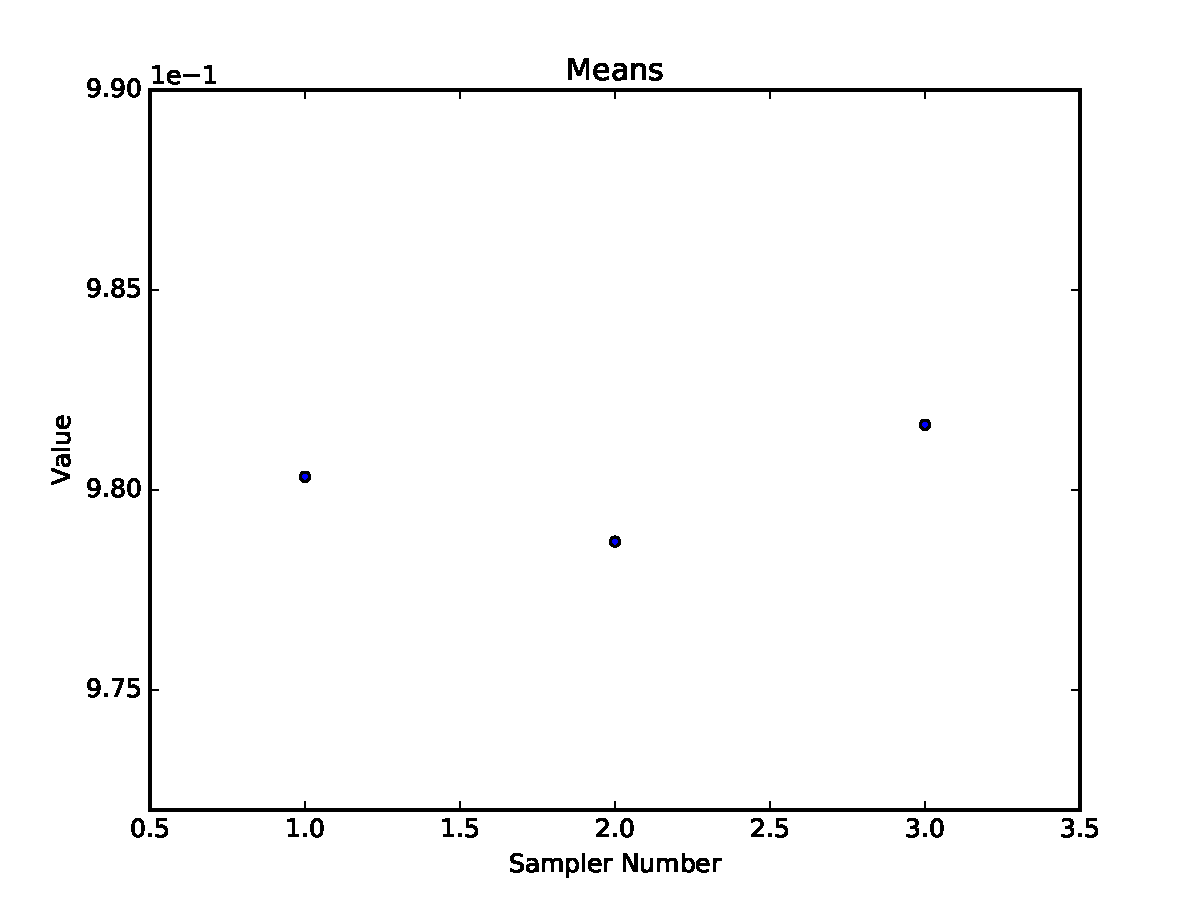
\includegraphics[width=0.7\linewidth]{../../tests/framework/user_guide/StatisticalAnalysis/comparingSamplers/meanPlotter_scatter}
  \caption{Sampler Comparison Plot, Means}
\end{figure}
\begin{figure}[h!]
  \centering
  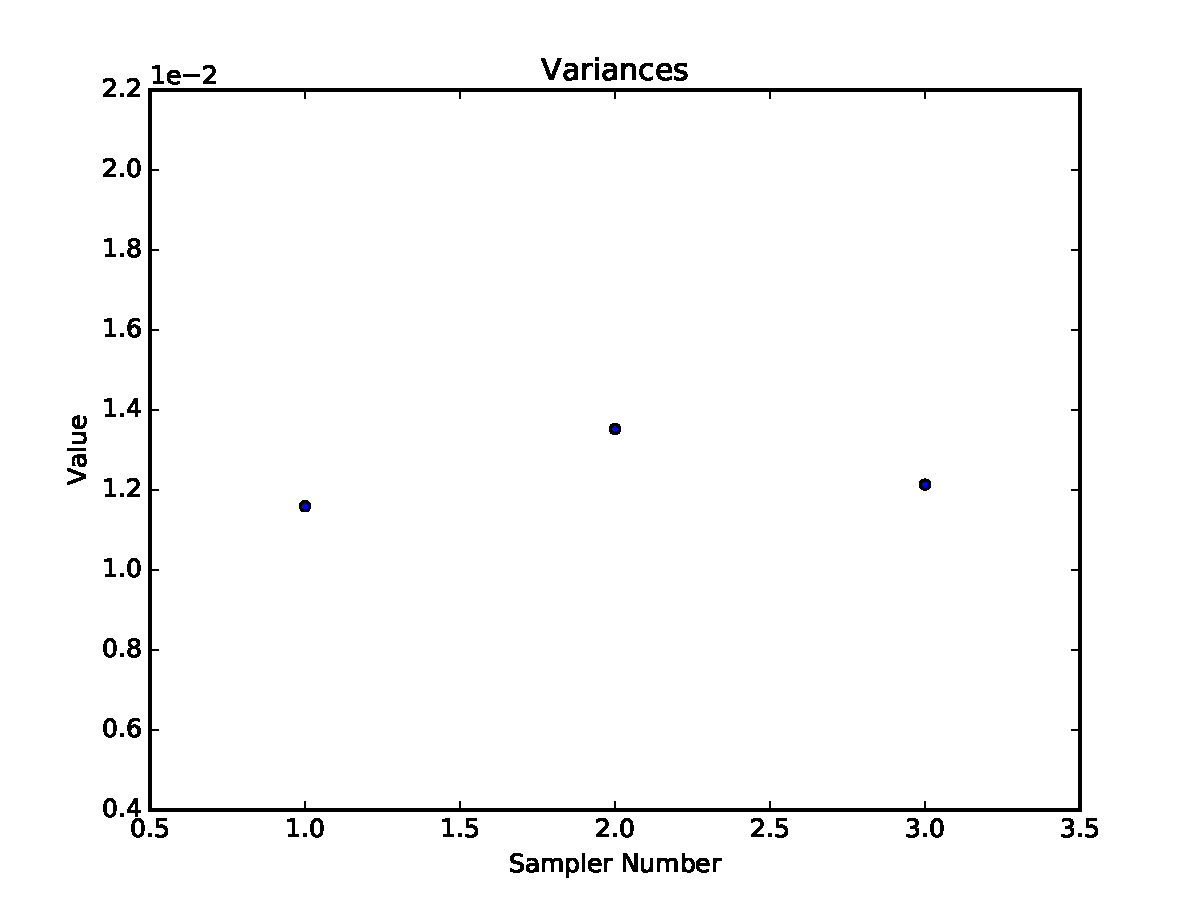
\includegraphics[width=0.7\linewidth]{../../tests/framework/user_guide/StatisticalAnalysis/comparingSamplers/varPlotter_scatter}
  \caption{Sampler Comparison Plot, Variance}
\end{figure}



\section{Data Mining through RAVEN}
\label{sec:DMraven}

Data mining is the computational process of discovering patterns in large data sets (``big data'') involving methods at the intersection of artificial intelligence, machine learning, statistics, and database systems. The overall goal of the data mining process is to extract information from a data set and transform it into an understandable structure for further use.
\\RAVEN has support of several different data mining algorithms,
such as:
\begin{enumerate}
  \item \textit{Hierarchical methodologies}
  \item \textit{K-Means}
  \item \textit{Mean-Shift}, etc.
\end{enumerate}

The goals of this section are about learning how to:
 \begin{enumerate}
   \item Set up a sampling strategy to apply clustering algorithms, perturbing a driven code
  \item Analyze the data using clustering algorithms.
\end{enumerate}
To accomplish these tasks, the following RAVEN \textbf{Entities} (XML blocks in the input files) need to be defined:
\begin{enumerate}
   \item \textbf{\textit{RunInfo}}:
     \xmlExample{framework/user_guide/DataMining/dataMiningAnalysis.xml}{RunInfo}
   The \textit{RunInfo} \textbf{Entity} is intended  to set up the analysis sequence that
   needs to be performed. The number of steps specified in (\xmlNode{Sequence}) are sequentially run
   using the number of processors assigned in (\xmlNode{batchSize}).
   \\In the first step, the original physical model is going to be sampled.
   The obtained results are going to be analyzed with data mining
   algorithms.
   \item \textbf{\textit{Models}}:
     \xmlExample{framework/user_guide/DataMining/dataMiningAnalysis.xml}{Models}
 The goal of this example is to show how the
 data mining algorithms in RAVEN can be useful to analyze large data set.
 \\In addition to an External model, two Post-Processor models ($DataMining|cluster|KMeans$ and $DataMining|decomposition|PCA$) are specified. Note that the post-processing is performed on all the output FOMs used in this example ($r and t$).
   \item \textbf{\textit{Distributions}}:
     \xmlExample{framework/user_guide/DataMining/dataMiningAnalysis.xml}{Distributions}
  In the Distributions XML section, the stochastic model for the
  uncertainties are reported. In this case 2 distributions are defined:
  \begin{itemize}
    \item $vel_dist \sim \mathbb{N}(30,5)$, used to model the uncertainties
    associated with  the \textit{velocity};
    \item  $angle_dist \sim \mathbb{U}(5,85)$,  used to
    model the uncertainties associated with the \textit{angle}.
  \end{itemize}
   \item \textbf{\textit{Samplers}}:
     \xmlExample{framework/user_guide/DataMining/dataMiningAnalysis.xml}{Samplers}
  In order to obtain the data-set on which the data mining algorithms are going to be applied, a \textit{MonteCarlo} sampling approach is employed here.
   \item \textbf{\textit{DataObjects}}:
     \xmlExample{framework/user_guide/DataMining/dataMiningAnalysis.xml}{DataObjects}
  In this block, three \textit{DataObjects} are defined:
  1) PointSet named ``samples'' used to collect the final outcomes of
  the code,
  2) PointSet named ``dummyIN'' used as a placeholder for the \textit{Multirun} step,
  3) HistorySet named ``histories'' in which the full time responses of the
  variables $x,y,t$ are going to be stored.
 %figure samples
 \begin{figure}[h!]
  \centering
  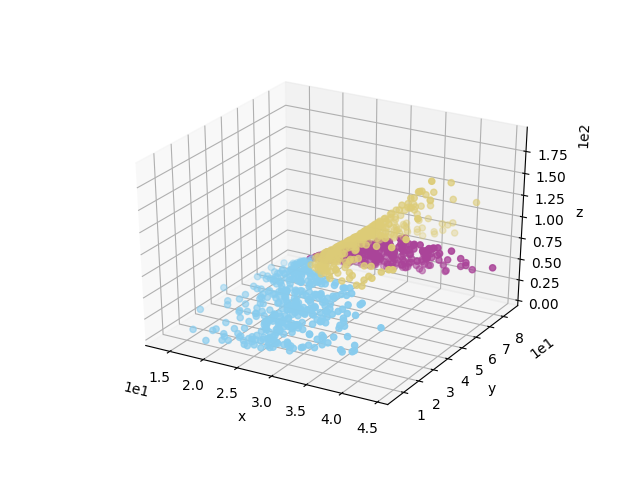
\includegraphics[scale=0.7]{../../tests/framework/user_guide/DataMining/gold/dataMiningAnalysis/1-PlotLabels_dataMining.png}
  \caption{K-means clustering on original dataset.}
  \label{fig:KmeanOrigData}
 \end{figure}
   \item \textbf{\textit{OutStreams}}:
     \xmlExample{framework/user_guide/DataMining/dataMiningAnalysis.xml}{OutStreams}
     This workflow uses one Print OutStream and three Plot OutStreams:
     \begin{itemize}
       \item ``samplesDump'', which writes the original sample set with the additional columns from the
         PostProcess steps,
       \item ``PlotKMeans1'', which plots the samples against the Figures of Merit with coloring according to the KMeans clustering,
       \item ``PlotLabels'', which plots the samples and colors them according to the KMeans clustering,
       \item ``PlotPCA1,'' which plots the surrogate principal component dimensions and their associated clustering.
     \end{itemize}
     Note that a special kind of plot, the ``dataMining'' \xmlNode{type}, has been implemented to simplify plotting complicated results using RAVEN, and is used in all three of the plots in this workflow.  Also note the use of the \xmlNode{range} block to define the data range of the plots created.
   \item \textbf{\textit{Steps}}:
     \xmlExample{framework/user_guide/DataMining/dataMiningAnalysis.xml}{Steps}

 %%%%%%%%%%%%%%%%%%%%%%%%%%%%%%%%%%%%%%%%%%%%%%%%%%%%%%%%%%
 %%%%%%%%%%%%%%%%%%%%%%%%%%%%%%%%%%%%%%%%%%%%%%%%%%%%%%%%%%
   Finally, all the previously defined \textbf{Entities} can be combined in
   the \xmlNode{Steps} block;
   3 \xmlNode{Steps} have been inputted:
   \begin{itemize}
     \item \xmlNode{MultiRun} named ``sample'', used to run the
     multiple
     instances of the driven code and
     collect the outputs in the two \textit{DataObjects}.The \xmlNode{Sampler} is inputted to communicate to the
     \textit{Step} that the driven code needs to
     be perturbed through the MonteCarlo sampling strategy;
     \item \xmlNode{PostProcess} named ``kmeans'', used
     to analyze the data obtained through the sampling strategy. In
     this step, a K-Means algorithm is going to be employed, plotting
     the clustering results;
     \textit{Step} that the driven code needs to
     be perturbed through the MonteCarlo sampling strategy;
     \item \xmlNode{PostProcess} named ``pca'', used
     to analyze the data obtained through the sampling strategy. In
     this Step, a PCA algorithm is going to be employed, plotting
     the decomposition results.
   \end{itemize}
\end{enumerate}
Figure~\ref{fig:KmeanOrigData} shows the clustering on the input space and the range, coloring according to the KMeans clustering,.
\\Figure~\ref{fig:KmeanProjected} shows the clustering on the range-angle and range-velocity plots respectively.
\\Figure~\ref{fig:PCAplot} shows the PCA decomposition on the data set.
%%%%%%%%%%%%%%%%%%%%%%%%%%%%%%%%%%%%%%%%%%%%%%%%%%%%%%%%%%
 %figure samples
 \begin{figure}[h!]
  \centering
  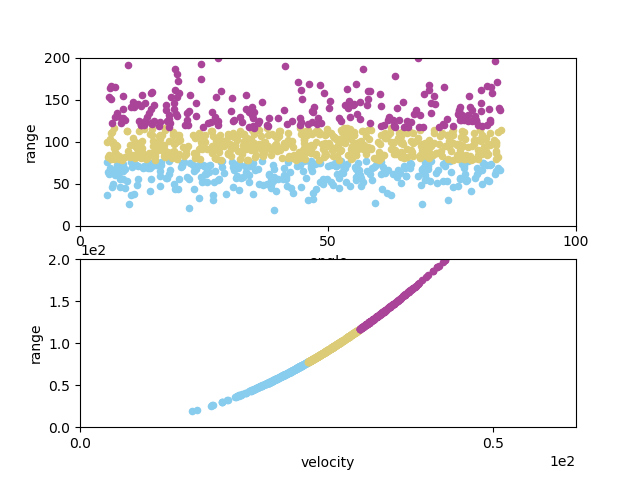
\includegraphics[scale=0.7]{../../tests/framework/user_guide/DataMining/gold/dataMiningAnalysis/1-PlotKMeans1_dataMining-dataMining.png}
  \caption{K-means clustering on projected parameters.}
  \label{fig:KmeanProjected}
 \end{figure}
 %%%%%%%%%%%%%%%%%%%%%%%%
 %%%%%%%%%%%%%%%%%%%%%%%%%%%%%%%%%%%%%%%%%%%%%%%%%%%%%%%%%%

 %%%%%%%%%%%%%%%%%%%%%%%%
  %%%%%%%%%%%%%%%%%%%%%%%%%%%%%%%%%%%%%%%%%%%%%%%%%%%%%%%%%%
 %figure samples
 \begin{figure}[h!]
  \centering
  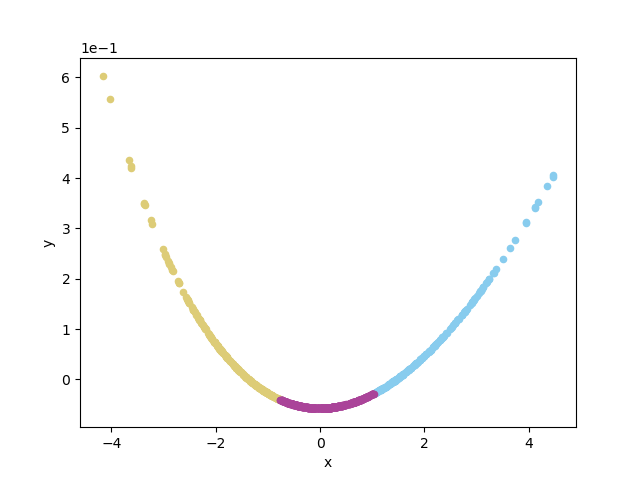
\includegraphics[scale=0.7]{../../tests/framework/user_guide/DataMining/gold/dataMiningAnalysis/1-PlotPCA1_dataMining.png}
  \caption{Principal Component Analysis.}
  \label{fig:PCAplot}
 \end{figure}
 %%%%%%%%%%%%%%%%%%%%%%%%


\section{Model Optimization}
\label{sec:optimizerStrategies}

When analyzing the range of values obtainable by a model, frequently a key question is ``what set of
parameters result in the best response value?''  To answer this question, RAVEN uses the \xmlNode{Optimizer},
a powerful sampler-like entity that searches the input space to find minimum or maximum values of a response.

In the remainder of this section, we will explore how to use the optimizer using a simple analytic problem,
with a two-dimensional input space and single response of interest.  After getting used to running with the
optimizer, we will add increasing complexity, including changing adaptive step sizes, initial conditions,
parallel trajectories, input space subdivision, input space constraints, and response constraints.

To demonstrate the operation of the Optimizer entities in RAVEN, the model we consider is the Beale function,
which is documented in the analytic tests for RAVEN and replicated here:

\begin{itemize}
  \item Function: $f(x,y) = (1.5-x+xy)^2+(2.25-x+xy^2)^2+(2.625-x+xy^3)^2$
  \item Domain: $-4.5 \leq x,y \leq 4.5$
  \item Global Minimum: $f(3,0.5)=0$
\end{itemize}

The two inputs are the variables $x$ and $y$, and the response is a value we'll assign to $ans$, short for
``answer''.  The model is an external model in RAVEN, and can be found at
\begin{verbatim}
  raven/tests/framework/AnalyticModes/optimizing/beale.py.
\end{verbatim}
The function's values are distributed as in Fig. \ref{fig:beale}.
\begin{figure}[h!]
  \centering
  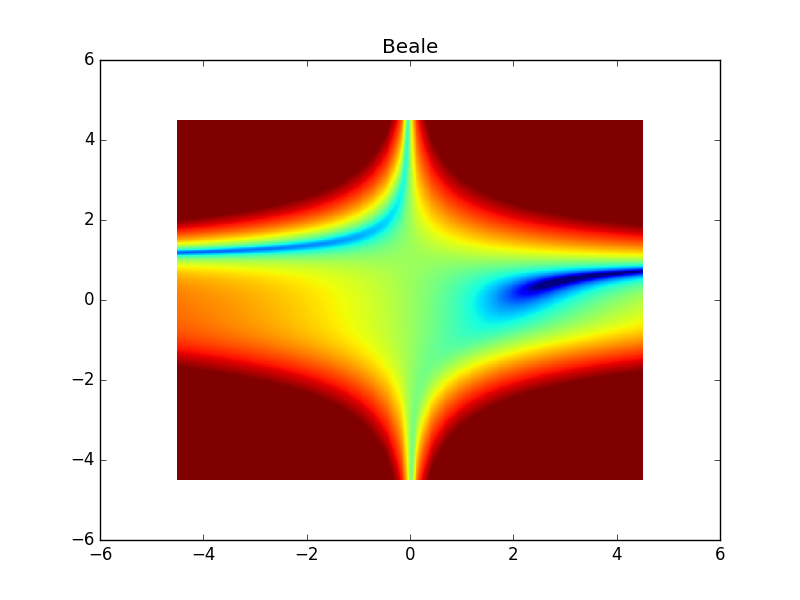
\includegraphics[scale=0.7]{../../tests/framework/user_guide/optimizing/Beale_grid.png}
  \caption{Plot of Beale's function for Optimization}
  \label{fig:beale}
\end{figure}

Note that throughout this example we use the SPSA optimizer by way of demonstration, since it is the first
advanced algorithm for optimization included in RAVEN; many of the options and parameters apply to other
optimizers, and details can be found in the RAVEN user manual.

\subsection{Introduction: The Optimizer Input}
As with other entities, the Optimizer gets its own XML block in the RAVEN input.
Here's an example of an input for a SPSA optimizer named \xmlString{opter}:
\xmlExample{framework/user_guide/optimizing/simple.xml}{Optimizers}
This is the smallest amount of input needed to run an optimization problem, with the exception that we include
the \xmlNode{initialSeed} to maintain consistent results.  Note the required blocks included
to define the optimizer:
\begin{itemize}
  \item \xmlNode{TargetEvaluation}, which declares the DataObject that the optimization search evaluations are
    going to be placed in.  All of the optimal points found as part of the optimization, as well as any other
    points evaluated as part of the algorithm, are placed in this object so the optimizer can retrieve this
    information later.  When this data object is defined, it is critical that the objective variable is
    defined in the output space, and the input variables in the input space, so the optimizer can collect the
    results of its sampling.  The data object type should be ``PointSet'' for this data object.  In this
    example, we use the self-descriptive \emph{optOut} data object.
  \item \xmlNode{variable}, which is where you can define the input space variables, one for each of these
    nodes.  Declaring a variable here informs the optimizer that you want it to find the optimal value for
    this variable, along with the other variables declared in their own blocks.  Additionally, you define the
    upper and lower bounds of the variable, which will give the optimizer some general expectations for
    finding the optimal point; it will never try to sample a value smaller than the lower bound or larger than
    the upper bound.  In the example we define variables \emph{x} and \emph{y} as our input variables, and
    both of them coincidentally range between -4.5 and 4.5.  We set the initial values for both variables to 0
    through the \xmlNode{initial} block, which is required in most cases; the exception is when a
    preconditioner sets them in mulitlevel optimization, but we're not concerned with that feature at this
    point.
  \item \xmlNode{objectVar}, which is where you indicate the variable for which you want to find the minimum (or,
    if you change the default, maximum).  As listed here, we want to minimize the value of \emph{ans} given a
    range of possible values for {x} and {y}.
\end{itemize}
The other critical blocks in this input are as follows:

\subsubsection{Models}
\xmlExample{framework/user_guide/optimizing/simple.xml}{Models}
Note that we define the external model with the name \xmlString{beale} and provide a path to the analytic
model itself.  This model is set up with the \texttt{run} method that allows RAVEN to run the model.  We also
list all our input/output variables, \emph{x, y}, and \emph{ans}.

\subsubsection{Data Objects}
\xmlExample{framework/user_guide/optimizing/simple.xml}{DataObjects}
We have three data objects: \xmlString{dummyIN}, which is necessary to define the input space of our external
model in the Steps; \xmlString{optOut}, which will hold all of the samples taken by our optimizer; and
\xmlString{opt\_export}, which will hold the actual solution path taken by our optimizer.  Note that while
\xmlString{optOut} is a Point Set, \xmlString{opt\_export} is a History Set.  This is because we store the
path travelled by the optimization algorithm as a history, with \emph{varsUpdate} keeping track of the
optimization steps taken.  Note especially how the input of \xmlString{opt\_export} is set to \emph{trajID},
which is a special keyword for the Optimizer history tracking, as is the output variable \emph{varsUpdate}.
There are several other special keyword outputs that can be written to the Solution Export data object, that
can be found in the user manual.

\subsubsection{Out Streams}
\xmlExample{framework/user_guide/optimizing/simple.xml}{OutStreams}
Here we define the way to print the output of our optimization algorithm.  There's not much to note, except
that we'll be printing the optimization path as a History-based CSV.

\subsubsection{Steps}
\xmlExample{framework/user_guide/optimizing/simple.xml}{Steps}
Here we put it all together into a work flow that RAVEN can follow.  We only need two steps: one to optimize,
and one to print out the results.  To actually perform the optimization, we need a MultiRun step, which we
cleverly name \xmlString{optimize}.  For input we take the placeholder data object \emph{dummyIN}, which sets
up the input space of the model we defined, \emph{beal}.  Where a \xmlNode{Sampler} would normally go, we
include the \xmlNode{Optimizer} we defined earlier.  We output to the same data object we indicated in the
Optimizer's \xmlNode{TargetEvaluation} node.  Finally, we note specifically the use of the
\xmlNode{SolutionExport} node.  The data object defined in this node is where the Optimizer will write the
optimization path history, with the final entry being the last step taken by the optimizer.  The IOStep is
unremarkable, used simply to write out the optimization path history to file.

\subsubsection{Conclusion}
After reviewing the components (don't forget the RunInfo block!), you can run this example and see the
results.  In particular, we can view the history of the optimizer in \texttt{Simple/opt\_export\_0.csv}.  Note
that \texttt{opt\_export} is the name of the \xmlNode{Print} OutStream we defined in the input file, and the
\texttt{\_0} indicates this is the first optimization path followed (we'll cover multiple paths later in
section \ref{subsec:opt parallel traj}).

When we open the file (preferably in a CSV reader such a spreadsheet viewer), we see a CSV with four headers,
the outputs defined in the data object in the input
file: \emph{x}, \emph{y}, \emph{ans}, and \emph{varsUpdate} (not necessarily in that order).  \emph{x},
\emph{y}, and \emph{ans} are the values of the variable at each optimization iteration, while
\emph{varsUpdate} gives the sequential order of the optimization iteration.

If we look at the last line, we converged around $f(1.61, -0.189) = 1.67$, which is okay but still quite a
ways from the analytic optimal point $f(3, 0.5) = 0$.  If we look at the output from the run, we can look at
the last time RAVEN was ``Checking convergence for Trajectory 0''.  Below that statement, there are a series
of convergence criteria and their status.  We can see that the reason we converged at the end is the
\texttt{Relative Loss Diff}, which means the relative change in the response \emph{ans} was sufficiently
small between steps to cause convergence.  Clearly, we claimed convergence prematurely because of the default convergence
values used by the optimizer.  Because these convergence criteria are very problem-specific, the default
parameters will not work best for all problems.

We can improve this result by changing convergence
parameters as well as step size growth and shrink factors, all of which can be found in the user manual, and
many of which we'll discuss in the rest of this section.

\subsection{Initial Conditions and Parallel Trajectories} \label{subsec:opt parallel traj}
Notice we set the optimization search to start at $(0,0)$.
%By default, RAVEN chooses the center
%point of the input space as an initial value.
You can change this initial value through
the \xmlNode{initial} block within the \xmlNode{variable} definition node.

Furthermore, RAVEN offers the possibility to run multiple optimization paths in parallel.  Because many
(perhaps most) optimization techniques get stuck in local minima, using multiple paths (or \emph{trajectories} as
they are called in RAVEN) increases the likelihood that one of the trajectories will find the global minimum
point.  You can request multiple trajectories by providing a variety of initial conditions in the
\xmlNode{initial} block, as shown in this Optimizer example:
\xmlExample{framework/user_guide/optimizing/multiple_trajectories.xml}{Optimizers}
Note that the ordered pairs are split across the \xmlNode{initial} nodes, so that the first trajectory will
start as a point made up of all the first entries, the second trajectory starts at all the second entries, and
et cetera.  In this case, we've requested starting points at (-2,-2), (-2,2), (2,-2), and (2,2).  This (and
defining a new working directory in the \xmlNode{RunInfo} block) is the only input change between the original
file and this one.

When run, we can see the results in the working directory \texttt{MultipleTraj}.  There, we see the same files
as for the base case, plus \texttt{opt\_export} files 0-3 instead of just 0.  Each of these corresponds to the
path that one of the initial points started at, as you can see at the top of each of these CSV files.  We can
see that trajectory 3 (who started at (2,2)) ended close to the analytic optimal point, while trajectory 0
was far from it.

In order to see a summary of the end point of each trajectory, we can use the additional RAVEN step described
in \ref{subsec:opt summarizing results}.


\subsection{Summarizing Results} \label{subsec:opt summarizing results}
While seeing the histories of the optimization paths taken in the \xmlNode{SolutionExport} is informative,
sometimes we just want to see the final optimal point found by each trajectory.  In this case, we can use an
\emph{InterfacedPostProcessor} called {HistorySetSnapShot} to get the last point found by each optimizer.  The
postprocessor looks like this:
\xmlExample{framework/user_guide/optimizing/summary.xml}{Models.PostProcessor}
Note that we named the postprocessor \xmlString{snapshot}, and instructed it to look for the \xmlString{max}
value of \xmlString{varsUpdate} in each of the histories, and combine them into a single data set.  We add the
following Step to our \xmlNode{Steps} to run it:
\xmlExample{framework/user_guide/optimizing/summary.xml}{Steps.PostProcess}
Don't forget to add \xmlString{getOptPoint} to the \xmlNode{Sequence} in the \xmlNode{RunInfo} block, before
\xmlString{print} but after \xmlString{optimize}.  Note that this post-processing step takes the
\xmlNode{SolutionExport} data object from the optimizing step as input, runs the postprocessing model, then
places the results in a new data object, \xmlString{opt\_soln}, which we add to the \xmlNode{DataObjects}
list in the input file.

Note also that we added the printing of the \xmlString{opt\_soln} data object to the \xmlString{print}
\xmlNode{IOStep}; we only needed to write an \xmlNode{OutStream} for it, not a whole new step.

After running this input, you can open \texttt{Summary/opt\_soln.csv} to see the final results of each
optimization trajectory.  The variable \emph{trajID} gives the trajectory label, \emph{x} and \emph{y} give
the final location of the optimal point found by that trajectory, \emph{ans} gives the value of the response
at that location, and \emph{varsUpdate} shows how many iterations were necessary to find that optimal point.
The trajectory with the lowest value for \emph{ans} is the most optimal point found.

\subsection{Adjusting Adaptive Steps} \label{subsec:opt stepsize}
As we've seen, some of the optimization paths are struggling to converge to meaningful optimal solutions.
One way to improve this is to tinker with the convergence tolerances defined in the user manual.  Another is
to change the step size modifications used as part of the search process, which we discuss in this section.
First, we briefly discuss how the SPSA chooses its step size, so we can make informed choices about what
parameters to use.

Because SPSA is a gradient-based method, it operates by starting at a particular point, estimating the
gradient at that point, then taking a step in the opposite direction of the gradient in order to follow a
downhill path.  It adaptively chooses how long of a step to take based on its history.  If the gradient is in
the same direction twice in a row, the algorithm assumes there's further to travel, so increases its step size
multiplicatively by the \emph{grainGrowthFactor}, which by default is 2.0 in RAVEN.  If, on the other hand,
the gradient switches directions, then the step size is divided by the \emph{gainShrinkFactor}, which again is
2.0 by default in RAVEN.  This means that by default, if the gradient keeps going in the same direction, you
always double your step size, while if you're bouncing back and forth in a valley, the step size is halved at
each iteration.

By way of note, in higher dimensions, the actual growth or shrink multiplier is scaled by a dot product
between the two previous gradients, with a max of the grain growth factor when the dot product is 1 (exactly
aligned) and a minimum of grain shrink factor when the dot product is -1 (exactly opposite).  This means if
the gradient is at right angles with the past gradient, then the step size remains unchanged (dot product is
0).

There are some additional considerations for the step size change, as well.  If the algorithm takes a step,
then discovers the new point has a worse response value than the point it's at, it will reject the new point,
re-evaluate the gradient, and flag the step size to be divided by the gain shrink factor.  Because of this, if
the gain shrink factor is too large, false convergence can be obtained when the algorithm struggles to find a
new downhill point to move to.  As a result, in practice it is often beneficial to have a gain shrink factor
that is smaller than the gain growth factor.

For this particular example, we use gain growth factor of 1.5 (meaning when the gradient continues in the same
direction our step grows to 150\% of its old value) and a gain shrink factor of 1.25 (meaning when the
gradient flips directions our step size shrinks to 80\% of its old value).  We add this to the base case
(\texttt{simple.xml}) to get:
\xmlExample{framework/user_guide/optimizing/step_size.xml}{Optimizers}
Note the definition of the gain growth and shrink factors in the \xmlNode{convergence} block.  Reviewing the
output file \texttt{StepSize}, we can see more steps were taken than the case using default step sizes, but
the final solution was $f(2.65,0.403)=0.0286$, which is much closer to the analytical solution of $f(3,0.5)=0$
than the base case and within our convergence tolerances of the right solution.

It is often challenging to find the best gain growth and shrink factors, and these can have a very significant
impact on the speed and accuracy of the convergence process.  Too large a shrink factor results in poor
resolution of valleys, while too small a shrink factor results in many unnecessary evaluations of the model.

\subsection{Denoising Stochastic Problems}
While many of the models we see in optimization are deterministic (meaning running the same inputs into the
model yields the same results every time), there are quite a few stochastic models that we might desire to
optimize.  For example, a model that included Brownian motion or is solved using unseeded random numbers might
be considered stochastic.

The difficulty with optimizing noisy problems rests in the unreliability of a single sample.  If we send a
single set of inputs into a stochastic model, we can't trust the results to be consistent.  One way to measure
the consistency of the results is through a signal-to-noise ratio (SNR).  There are many ways to define this
value; for our purposes, we will use the ratio of the mean of the signal to the standard deviation of the
signal, $\mu/\sigma$.

To obtain an approximation of your SNR, you can use RAVEN to perform a Monte Carlo run on your model and then
use the BasicStatistics postprocessor to collect the mean (expectedValue) and standard deviation (sigma) of
your response.  It's important to make this sampling all at a single value in the input space, so replace your
variables with constants in the Sampler input.  Once you have the mean and sigma, you have an idea of how
noisy your model is.  A SNR of 1 means the signal is just as big as the noise, making it very difficult to
optimize.  A SNR of less than 1 means the noise dominates the signal, and will make optimization almost
impossible without introducing denoising.  A SNR of more than 1 indicates the signal is stronger than the
noise, and perhaps denoising is not necessary.  If your standard deviation is 0, then you don't have any
discernable noise!

To denoise a model in RAVEN SPSA optimization currently, we turn our attention to the \xmlNode{Optimizer}
subnode \xmlNode{parameter}, specifically the \xmlNode{numGradAvgIterations} node.  This parameter instructs
RAVEN to perform multiple gradient evaluations, including multiple evaluations of each optimal point, and use
the average to make decisions in optimization pathing.  By default, RAVEN takes one optimal point and one
neighboring point to evaluate a gradient.  Increasing the \xmlNode{numGradAvgIterations} will increase the
number of times the optimal point is sampled, and how many neighbor points are sampled.  This serves to
denoise the model.

However, this also raises the question, how many resamples do I need to denoise my model?  In a Wilks-like
approach, we want to reduce the size of the confidence interval for our mean to be less than the noise.  The
number of resamples required depends on the size of the confidence interval $z$ and the confidence-to-noise ratio
$\xi$ we want to ultimately have for the optimization algorithm.  We also assume the distribution of the
response is roughly Gaussian Normal, which may not be the case.  The approximate equation for assuring the
confidence interval is smaller than the noise is
\begin{equation}
  \frac{z\sigma}{\sqrt{n}} \leq \xi\sigma,
\end{equation}
\begin{equation}
  n \geq \left(\frac{z}{\xi}\right)^2.
\end{equation}
Thus, the number of resamples depends on the confidence level as well as the desired ratio of the confidence interval
to the noise.

A few values for varying ratios are given in Table \ref{tab:confidence levels} for the 99\% confidence level ($z=2.576$).
\begin{table}[htb]
  \centering
  \begin{tabular}{c c}
    Confidence-to-noise $\xi$ & Resamples necessary \\ \hline
    1.0 & 7 \\
    0.9 & 9 \\
    0.7 & 14 \\
    0.5 & 27 \\
    0.1 & 664 \\
    0.05 & 2655
  \end{tabular}
  \caption{Estimate of the number of samples necessary to denoise models to varying confidence levels}
  \label{tab:confidence levels}
\end{table}
That is, if you want the noise and confidence interval to have the same magnitude, only 7 resamples are
required.  If, on the other hand, you want the confidence interval to be half the level of the noise, 27
resamples are required.

Note these are only guidelines; individual models may behave differently and require more or less resamples to
provide a clear optimization path.

\subsection{Input Space Subdivision}
In higher-dimensional problems, sometimes the input space can be divided into characteristic subspaces.  For
example, potentially one set of inputs vary slowly with consistent gradient directions in the response, while
for another set of inputs the response fluctuates frequently with many local minima.  In this case, it might
be beneficial to optimize the subspaces in nested loops, slowly converging the smoothly-varying space while
often converging the undulating space.

For these cases, RAVEN provides \emph{multilevel} operation.  To transition our base case to a multilevel
case, we change the optimizer as follows:
\xmlExample{framework/user_guide/optimizing/multilevel.xml}{Optimizers}
Note the addition of the \xmlNode{multilevel} node.  In this node, we need to define the subspaces, then the
ordering of the subspaces in terms of convergence priority.  We intuitively name the subspace with \emph{x}
the \emph{xgroup} and similarly with \emph{y}.  Note that while in this example each subspace consists of only
one variable, in general many variables may exist in any given subspace.  Note also that it's a bad idea to
include a variable in multiple subspaces.

The \xmlNode{sequence} can be thought of as an order of nesting optimization, where the first subspace listed
is optimized most slowly (but only once) and the last is optimized frequently and swiftly.  Each time a new
optimal point is found, the innermost space (in our example \emph{yspace}) is converged completely, holding all
the variables in all other subspaces (e.g. \emph{xspace}) constant at their most recent value.  Once
\emph{yspace} is converged, we take a single step in the subspace \emph{xgroup}, then return to converging
\emph{yspace} again.  Every step in \emph{xspace} triggers a full convergence of \emph{yspace}.

In the results in \texttt{Multilevel/opt\_export\_0.csv}, you can observe how first one dimension then the
other is perturbed in the search for the optimal point.

It should be noted as well, using multilevel optimization does not necessarily improve the optimization path;
in fact, in many cases, the number of model evaluations increases significantly for little gain in final
optimal value.  Multilevel is most useful when clustered subspaces share a particular feature in optimization
that is useful to isolate from the rest of the optimization procedure, or if some subsets of inputs act
independently from others in affecting the response.


\subsection{Functional Constraints} \label{subsec:opt explicit constraint}
Sometimes an optimization problem has a constrained input space, possibly where there is a tradeoff between
two inputs.  In this event, RAVEN allows the user to define a \emph{constraint} function, which will cause
RAVEN to treat this constraint as it would a boundary condition.

For example, we will introduce a void in the input where we reject inputs.  This void is defined by rejecting
all samples within $(x-1)^2 + y^2 < 1$.  We'll also include the modified step growth and shrink parameters
discussed in section \ref{subsec:opt stepsize}.

To include a constraint function, we first have to define it in the RAVEN input as a \xmlNode{Function}
entity:
\xmlExample{framework/user_guide/optimizing/constrain.xml}{Functions}
Note that the file \texttt{./Constrain/constraint.py} is located relative to the working directory.  Currently,
external functions are always Python files.  In that file,
note that the only method is \texttt{constrain}, which is RAVEN's keyword to find the constraint function.
RAVEN will pass in a \texttt{self} object, which will have the function variables defined in the
\xmlNode{Functions} input available as members.  The method \texttt{constrain} then returns a boolean which is \texttt{True} if
the evaluation does not violate the constraint, or \texttt{False} if the constraint is violated.

To attach the constraint to the optimizer, simply add it as an assembled \xmlNode{Function}:
\xmlExample{framework/user_guide/optimizing/constrain.xml}{Optimizers}

After running, looking through the path followed by trajectory 0 shows that instead of following the path from
section \ref{subsec:opt stepsize}, the path moves to lower \emph{y} values before swinging back up toward the
optimal point.

%\subsection{Implicit Constraints (Penalties)}
% TODO come up with a working example

\clearpage
\begin{appendices}
  %\section{Running RAVEN}
\label{HowToRun}

% I don't think this is mentioned earlier? Andrea answers :D It mentioned in the Introduction
%As already mentioned,
The RAVEN code is a blend of C++, C, and Python software. The entry point
resides on the Python side and is accessible via a command line interface.
%
After following the instructions in the previous Section, RAVEN is ready to be
used.
%
The \texttt{raven\_framework} script is in the raven folder.
%
To run RAVEN, open a terminal and use the following command (replace \texttt{<inputFileName.xml>} with your RAVEN input file):

\begin{lstlisting}[language=bash]
raven_framework <inputFileName.xml>
\end{lstlisting}

Alternatively, the \texttt{Driver.py} script can be directly used.  The RAVEN driver is contained in the folder ``\texttt{raven/framework}.'' In this case, the command is:

\begin{lstlisting}[language=bash]
python raven/framework/Driver.py <inputFileName.xml>
\end{lstlisting}


  \section{Document Version Information}
  d317572ffb80f564d27ec54e5db24d763705a8a5 Aaron Epiney - INL Tue, 17 Oct 2017 XX:XX:XX -0600

\end{appendices}
%\appendix
\section{Appendix: Example Primer}
\label{sec:examplePrimer}
In this Appendix, a set of examples are reported. In order to be as general as possible, the \textit{Model} type ``ExternalModel'' has been used.
%%%% EXAMPLE 1
\subsection{Example 1.}
\label{subsec:ex1}
This simple example is about the construction of a ``Lorentz attractor'', sampling the relative input space. The parameters that are sampled represent the initial coordinate (x0,y0,z0) of the attractor origin.

\begin{lstlisting}[style=XML,morekeywords={debug,re,seeding,class,subType,limit}]
<?xml version="1.0" encoding="UTF-8"?>
<Simulation verbosity="debug">
<!-- RUNINFO -->
<RunInfo>
    <WorkingDir>externalModel</WorkingDir>
    <Sequence>FirstMRun</Sequence>
    <batchSize>3</batchSize>
</RunInfo>
<!-- Files -->
<Files>
    <Input name='lorentzAttractor.py' type=''>lorentzAttractor</Input>
</Files>
<!-- STEPS -->
<Steps>
    <MultiRun name='FirstMRun'  re-seeding='25061978'>
        <Input   class='Files'     type=''               >lorentzAttractor.py</Input>
        <Model   class='Models'    type='ExternalModel'  >PythonModule</Model>
        <Sampler class='Samplers'  type='MonteCarlo'     >MC_external</Sampler>
        <Output  class='DataObjects'     type='HistorySet'      >testPrintHistorySet</Output>
        <Output  class='Databases' type='HDF5'           >test_external_db</Output>
        <Output  class='OutStreams' type='Print'   >testPrintHistorySet_dump</Output>
    </MultiRun >
</Steps>
<!-- MODELS -->
<Models>
    <ExternalModel name='PythonModule' subType='' ModuleToLoad='externalModel/lorentzAttractor'>
       <variables>sigma,rho,beta,x,y,z,time,x0,y0,z0</variables>
    </ExternalModel>
</Models>
<!-- DISTRIBUTIONS -->
<Distributions>
    <Normal name='x0_distrib'>
        <mean>4</mean>
        <sigma>1</sigma>
    </Normal>
    <Normal name='y0_distrib'>
        <mean>4</mean>
        <sigma>1</sigma>
    </Normal>
    <Normal name='z0_distrib'>
        <mean>4</mean>
        <sigma>1</sigma>
    </Normal>
</Distributions>
<!-- SAMPLERS -->
<Samplers>
    <MonteCarlo name='MC_external'>
      <samplerInit>
        <limit>3</limit>
      </samplerInit>
      <variable name='x0' >
        <distribution  >x0_distrib</distribution>
      </variable>
      <variable name='y0' >
        <distribution  >y0_distrib</distribution>
      </variable>
      <variable name='z0' >
        <distribution  >z0_distrib</distribution>
      </variable>
    </MonteCarlo>
</Samplers>
<!-- DATABASES -->
<Databases>
  <HDF5 name="test_external_db"/>
</Databases>
<!-- OUTSTREAMS -->
<OutStreams>
  <Print name='testPrintHistorySet_dump'>
    <type>csv</type>
    <source>testPrintHistorySet</source>
  </Print>
</OutStreams>
<!-- DATA OBJECTS -->
<DataObjects>
    <HistorySet name='testPrintHistorySet'>
        <Input>x0,y0,z0</Input>
        <Output>time,x,y,z</Output>
   </HistorySet>
</DataObjects>
</Simulation>
\end{lstlisting}
The Python \textit{ExternalModel} is reported below:
\begin{lstlisting}[language=python]
import numpy as np

def run(self,Input):
  max_time = 0.03
  t_step = 0.01

  numberTimeSteps = int(max_time/t_step)

  self.x = np.zeros(numberTimeSteps)
  self.y = np.zeros(numberTimeSteps)
  self.z = np.zeros(numberTimeSteps)
  self.time = np.zeros(numberTimeSteps)

  self.x0 = Input['x0']
  self.y0 = Input['y0']
  self.z0 = Input['z0']

  self.x[0] = Input['x0']
  self.y[0] = Input['y0']
  self.z[0] = Input['z0']
  self.time[0]= 0

  for t in range (numberTimeSteps-1):
    self.time[t+1] = self.time[t] + t_step
    self.x[t+1]    = self.x[t] +  self.sigma*
                      (self.y[t]-self.x[t]) * t_step
    self.y[t+1]    = self.y[t] + (self.x[t]*
                      (self.rho-self.z[t])-self.y[t]) * t_step
    self.z[t+1]    = self.z[t] + (self.x[t]*
                          self.y[t]-self.beta*self.z[t]) * t_step
\end{lstlisting}
%%%% EXAMPLE 2
\subsection{Example 2.}
\label{subsec:ex1}
This example shows a slightly more complicated example, that employs the usage of:
\begin{itemize}
    \item \textit{Samplers:} Grid and Adaptive;
    \item \textit{Models:} External, Reduce Order Models and Post-Processors;
    \item \textit{OutStreams:} Prints and Plots;
    \item \textit{Data Objects:} PointSets;
    \item \textit{Functions:} ExternalFunctions.
\end{itemize}
The goal of this input is to compute the ``SafestPoint''.
It provides the coordinates of the farthest
point from the limit surface that is given as an input.
%
The safest point coordinates are expected values of the coordinates of the
farthest points from the limit surface in the space of the ``controllable''
variables based on the probability distributions of the ``non-controllable''
variables.

The term ``controllable'' identifies those variables that are under control
during the system operation, while the ``non-controllable'' variables are
stochastic parameters affecting the system behavior randomly.

The ``SafestPoint'' post-processor requires the set of points belonging to the
limit surface, which must be given as an input.

\begin{lstlisting}[style=XML,morekeywords={debug,re,seeding,class,subType,limit}]
<Simulation verbosity='debug'>

<!-- RUNINFO -->
<RunInfo>
  <WorkingDir>SafestPointPP</WorkingDir>
  <Sequence>pth1,pth2,pth3,pth4</Sequence>
  <batchSize>50</batchSize>
</RunInfo>

<!-- STEPS -->
<Steps>
  <MultiRun name = 'pth1' pauseAtEnd = 'False'>
    <Sampler  class = 'Samplers'  type = 'Grid'           >grd_vl_ql_smp_dpt</Sampler>
    <Input    class = 'DataObjects'     type = 'PointSet'   >grd_vl_ql_smp_dpt_dt</Input>
    <Model    class = 'Models'    type = 'ExternalModel'  >xtr_mdl</Model>
    <Output   class = 'DataObjects'     type = 'PointSet'   >nt_phy_dpt_dt</Output>
  </MultiRun >

  <MultiRun name = 'pth2' pauseAtEnd = 'True'>
    <Sampler          class = 'Samplers'  type = 'Adaptive'      >dpt_smp</Sampler>
    <Input            class = 'DataObjects'     type = 'PointSet'  >bln_smp_dt</Input>
    <Model            class = 'Models'    type = 'ExternalModel' >xtr_mdl</Model>
    <Output           class = 'DataObjects'     type = 'PointSet'  >nt_phy_dpt_dt</Output>
    <SolutionExport   class = 'DataObjects'     type = 'PointSet'  >lmt_srf_dt</SolutionExport>
  </MultiRun>

  <PostProcess name='pth3' pauseAtEnd = 'False'>
    <Input    class = 'DataObjects'          type = 'PointSet'       >lmt_srf_dt</Input>
    <Model    class = 'Models'         type = 'PostProcessor'  >SP</Model>
    <Output   class = 'DataObjects'          type = 'PointSet'     >sfs_pnt_dt</Output>
  </PostProcess>

  <OutStreamStep name = 'pth4' pauseAtEnd = 'True'>
  	<Input  class = 'DataObjects'            type = 'PointSet'  >lmt_srf_dt</Input>
  	<Output class = 'OutStreams' type = 'Print'         >lmt_srf_dmp</Output>
    <Input  class = 'DataObjects'            type = 'PointSet'  >sfs_pnt_dt</Input>
  	<Output class = 'OutStreams' type = 'Print'         >sfs_pnt_dmp</Output>
  </OutStreamStep>
</Steps>

<!-- DATA OBJECTS -->
<DataObjects>
  <PointSet name = 'grd_vl_ql_smp_dpt_dt'>
    <Input>x1,x2,gammay</Input>
    <Output>OutputPlaceHolder</Output>
  </PointSet>

  <PointSet name = 'nt_phy_dpt_dt'>
    <Input>x1,x2,gammay</Input>
    <Output>g</Output>
  </PointSet>

  <PointSet name = 'bln_smp_dt'>
    <Input>x1,x2,gammay</Input>
    <Output>OutputPlaceHolder</Output>
  </PointSet>

  <PointSet name = 'lmt_srf_dt'>
    <Input>x1,x2,gammay</Input>
    <Output>g_zr</Output>
  </PointSet>

  <PointSet name = 'sfs_pnt_dt'>
    <Input>x1,x2,gammay</Input>
    <Output>p</Output>
  </PointSet>
</DataObjects>

<!-- DISTRIBUTIONS -->
<Distributions>
  <Normal name = 'x1_dst'>
    <upperBound>10</upperBound>
    <lowerBound>-10</lowerBound>
  	<mean>0.5</mean>
    <sigma>0.1</sigma>
  </Normal>

  <Normal name = 'x2_dst'>
    <upperBound>10</upperBound>
    <lowerBound>-10</lowerBound>
    <mean>-0.15</mean>
    <sigma>0.05</sigma>
  </Normal>

  <Normal name = 'gammay_dst'>
    <upperBound>20</upperBound>
    <lowerBound>-20</lowerBound>
    <mean>0</mean>
    <sigma>15</sigma>
  </Normal>
</Distributions>

<!-- SAMPLERS -->
<Samplers>
  <Grid name = 'grd_vl_ql_smp_dpt'>
    <variable name = 'x1' >
      <distribution>x1_dst</distribution>
      <grid type = 'value' construction = 'equal' steps = '10' upperBound = '10'>2</grid>
    </variable>
    <variable name='x2' >
      <distribution>x2_dst</distribution>
      <grid type = 'value' construction = 'equal' steps = '10' upperBound = '10'>2</grid>
    </variable>
    <variable name='gammay' >
      <distribution>gammay_dst</distribution>
      <grid type = 'value' construction = 'equal' steps = '10' lowerBound = '-20'>4</grid>
    </variable>
  </Grid>

  <Adaptive name = 'dpt_smp' verbosity='debug'>
    <ROM              class = 'Models'    type = 'ROM'           >accelerated_ROM</ROM>
    <Function         class = 'Functions' type = 'External'      >g_zr</Function>
    <TargetEvaluation class = 'DataObjects'     type = 'PointSet'  >nt_phy_dpt_dt</TargetEvaluation>
    <Convergence limit = '3000' forceIteration = 'False' weight = 'none' persistence = '5'>1e-2</Convergence>
      <variable name = 'x1'>
        <distribution>x1_dst</distribution>
      </variable>
      <variable name = 'x2'>
        <distribution>x2_dst</distribution>
      </variable>
      <variable name = 'gammay'>
        <distribution>gammay_dst</distribution>
      </variable>
  </Adaptive>
</Samplers>

<!-- MODELS -->
<Models>
  <ExternalModel name = 'xtr_mdl' subType = '' ModuleToLoad = 'SafestPointPP/safest_point_test_xtr_mdl'>
    <variables>x1,x2,gammay,g</variables>
  </ExternalModel>

  <ROM name = 'accelerated_ROM' subType = 'SciKitLearn'>
    <Features>x1,x2,gammay</Features>
    <Target>g_zr</Target>
    <SKLtype>svm|SVC</SKLtype>
    <kernel>rbf</kernel>
    <gamma>10</gamma>
    <tol>1e-5</tol>
    <C>50</C>
  </ROM>

  <PostProcessor name='SP' subType='SafestPoint'>
    <!-- List of Objects (external with respect to this PP) needed by this post-processor -->
    <Distribution     class = 'Distributions'  type = 'Normal'>x1_dst</Distribution>
    <Distribution     class = 'Distributions'  type = 'Normal'>x2_dst</Distribution>
    <Distribution     class = 'Distributions'  type = 'Normal'>gammay_dst</Distribution>
    <!- end of the list -->
    <controllable>
    	<variable name = 'x1'>
    		<distribution>x1_dst</distribution>
    		<grid type = 'value' steps = '20'>1</grid>
    	</variable>
    	<variable name = 'x2'>
    		<distribution>x2_dst</distribution>
    		<grid type = 'value' steps = '20'>1</grid>
    	</variable>
    </controllable>
    <non-controllable>
    	<variable name = 'gammay'>
    		<distribution>gammay_dst</distribution>
    		<grid type = 'value' steps = '20'>2</grid>
    	</variable>
    </non-controllable>
  </PostProcessor>
</Models>

<!-- FUNCTIONS -->
<Functions>
  <External name='g_zr' file='SafestPointPP/safest_point_test_g_zr.py'>
    <variable>g</variable>
  </External>
</Functions>

<!-- OUT-STREAMS -->
<OutStreams>
  <Print name = 'lmt_srf_dmp'>
  	<type>csv</type>
  	<source>lmt_srf_dt</source>
  </Print>

  <Print name = 'sfs_pnt_dmp'>
  	<type>csv</type>
  	<source>sfs_pnt_dt</source>
  </Print>
</OutStreams>

</Simulation>
\end{lstlisting}
The Python \textit{ExternalModel} is reported below:
\begin{lstlisting}[language=python]
def run(self,Input):
  self.g = self.x1+4*self.x2-self.gammay
\end{lstlisting}
The ``Goal Function'',the function that defines the transitions with respect the input space coordinates, is as follows:
\begin{lstlisting}[language=python]
def __residuumSign(self):
  if self.g<0 : return  1
  else        : return -1
\end{lstlisting}

%%%%% EXAMPLE 3
%\subsection{Example3}
%\label{subsec:ex1}
%example 3



    % ---------------------------------------------------------------------- %
    % References
    %
    \clearpage
    % If hyperref is included, then \phantomsection is already defined.
    % If not, we need to define it.
    \providecommand*{\phantomsection}{}
    \phantomsection
    \addcontentsline{toc}{section}{References}
    \bibliographystyle{ieeetr}
    \bibliography{raven_user_guide}


    % ---------------------------------------------------------------------- %
    %

    % \printindex

    %\include{distribution}

\end{document}
